% CONTINUACION DEL INFORME EXISTENTE (ramaFRANKI)
% Insertar antes de la seccion Conclusiones y Recomendaciones:
% % CONTINUACION DEL INFORME EXISTENTE (ramaFRANKI)
% Insertar antes de la seccion Conclusiones y Recomendaciones:
% % CONTINUACION DEL INFORME EXISTENTE (ramaFRANKI)
% Insertar antes de la seccion Conclusiones y Recomendaciones:
% % CONTINUACION DEL INFORME EXISTENTE (ramaFRANKI)
% Insertar antes de la seccion Conclusiones y Recomendaciones:
% \input{actualizacion_evidencias_noviembre}
% Usa paquetes ya presentes en main.tex: graphicx, float, booktabs, tabularx, subcaption.

\section{Actualización experimental: ensamble, conexiones y ajustes del manipulador}
\label{sec:actualizacion_evidencias}

\subsection{Objeto y alcance del registro fotográfico}
Las evidencias recopiladas corresponden a una nueva etapa de integración del brazo robótico articulado. Se observan diferentes configuraciones mecánicas del manipulador, el montaje de un controlador PWM PCA9685, un módulo de la familia ESP32, conexiones mediante cables y elementos empleados para evaluar la alimentación eléctrica. El propósito de esta sección es registrar el progreso físico del prototipo y delimitar las comprobaciones que aún se requieren. Las fotografías son evidencia de montaje, pero no constituyen por sí mismas una medida de precisión, par disponible o estabilidad eléctrica.

\subsection{Progreso del ensamblaje y postura de las articulaciones}
El manipulador conserva una estructura de eslabones rígidos, servomotores montados en soportes metálicos, pinza mecánica y base de madera. Las nuevas imágenes muestran posiciones inclinadas, frontales y casi verticales, útiles para observar la alineación relativa de hombro, codo y muñeca. Estas posiciones sirven como referencia para identificar posibles interferencias, puntos de holgura y distribución del cableado. No se dispone de un registro instrumental de los ángulos reales, por lo que la denominación ``calibración'' se emplea aquí para describir el proceso de ajuste y verificación, no para afirmar que haya concluido.

\begin{figure}[H]
 \centering
 \begin{subfigure}[t]{0.48\textwidth}
  \centering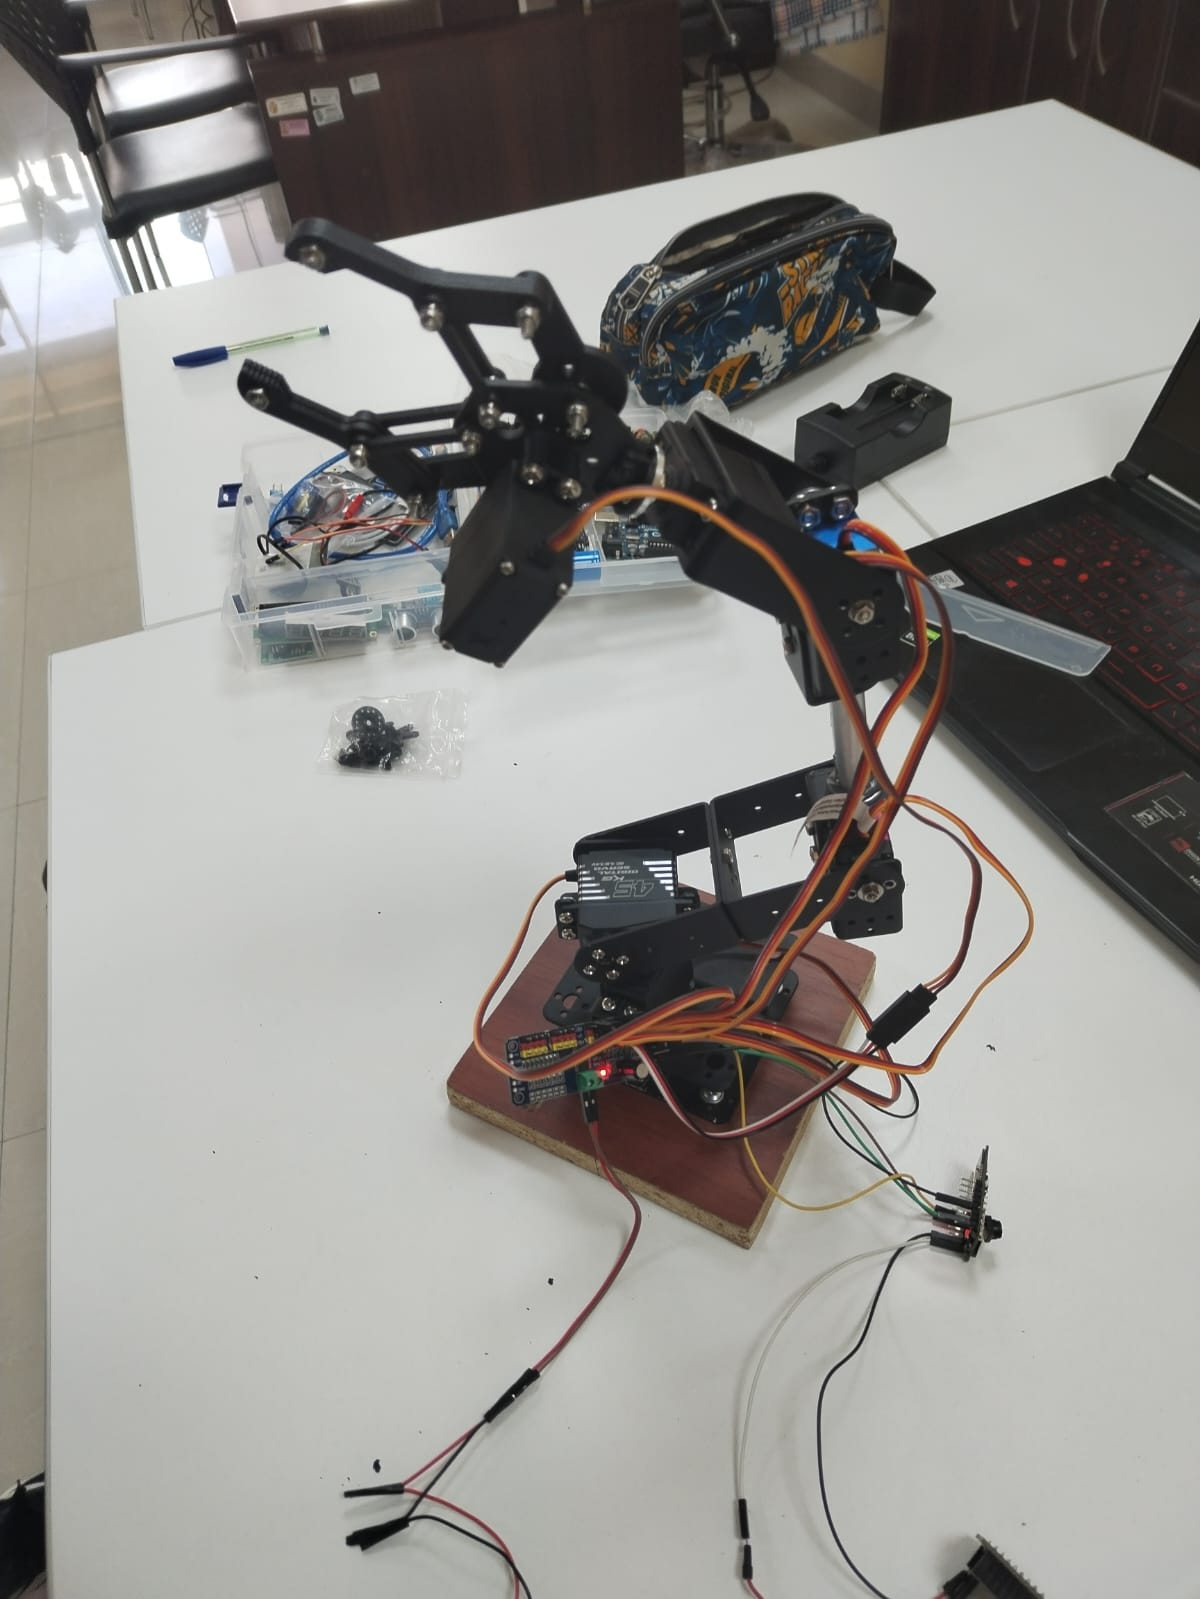
\includegraphics[width=\linewidth,height=7cm,keepaspectratio]{img/evidencia_brazo_integracion_lateral.jpg}
  \caption{Vista lateral durante la integración de la pinza y los eslabones.}
 \end{subfigure}\hfill
 \begin{subfigure}[t]{0.48\textwidth}
  \centering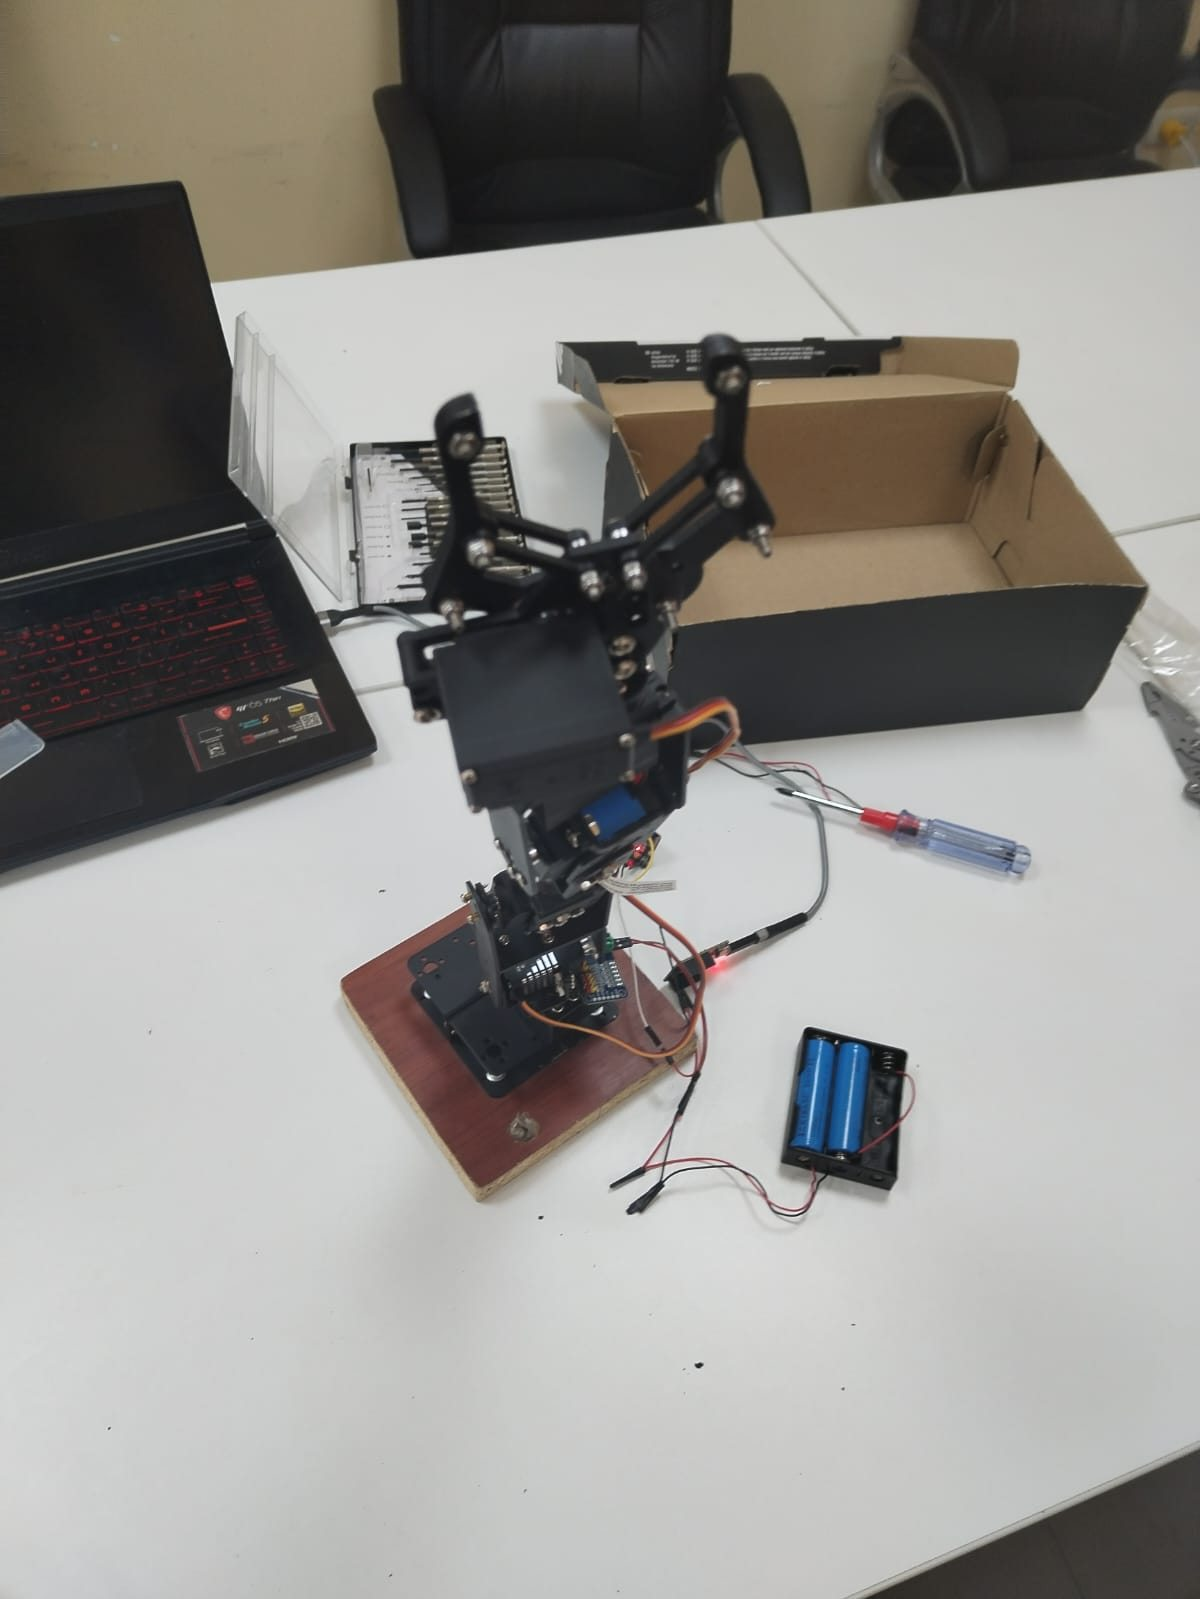
\includegraphics[width=\linewidth,height=7cm,keepaspectratio]{img/evidencia_brazo_vista_frontal.jpg}
  \caption{Vista frontal del conjunto articulado en banco de trabajo.}
 \end{subfigure}
 \caption{Registro del ensamble físico en diferentes orientaciones.}
 \label{fig:actualizacion_ensamble}
\end{figure}

\begin{figure}[H]
 \centering
 \begin{subfigure}[t]{0.48\textwidth}
  \centering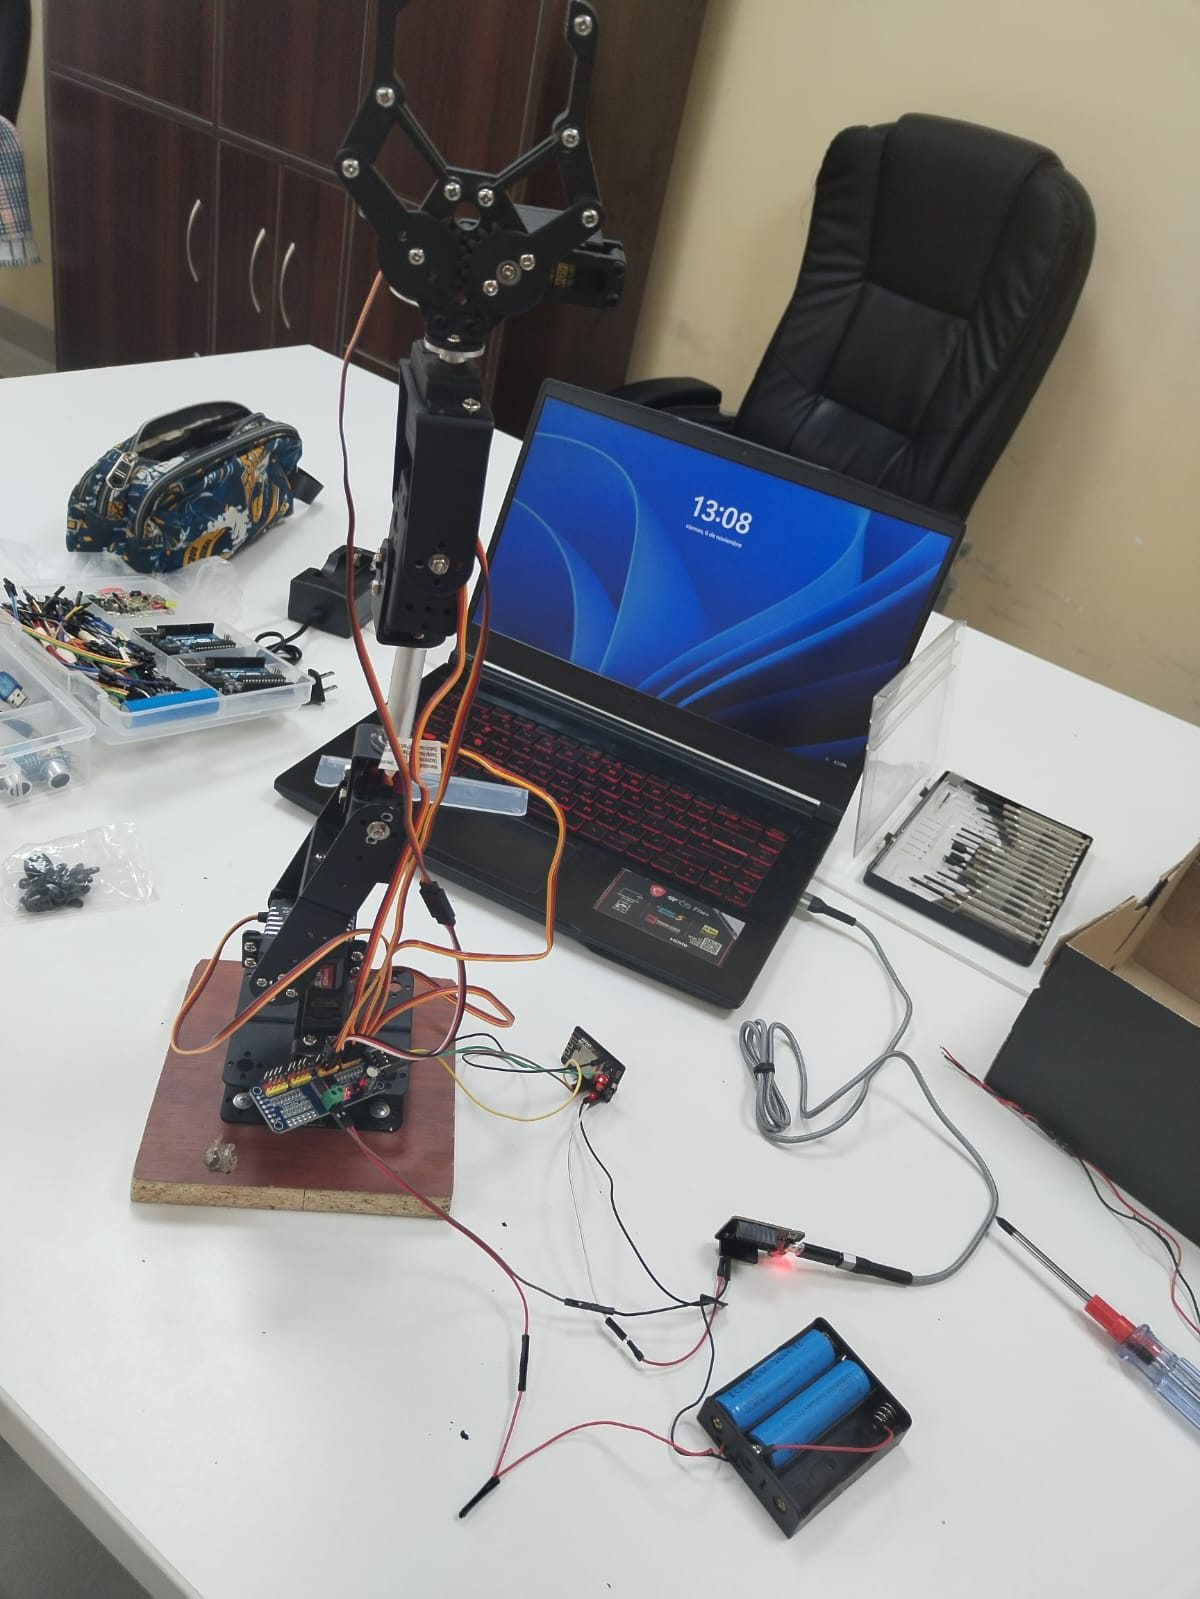
\includegraphics[width=\linewidth,height=7cm,keepaspectratio]{img/evidencia_brazo_postura_vertical.jpg}
  \caption{Prototipo con el efector final elevado.}
 \end{subfigure}\hfill
 \begin{subfigure}[t]{0.48\textwidth}
  \centering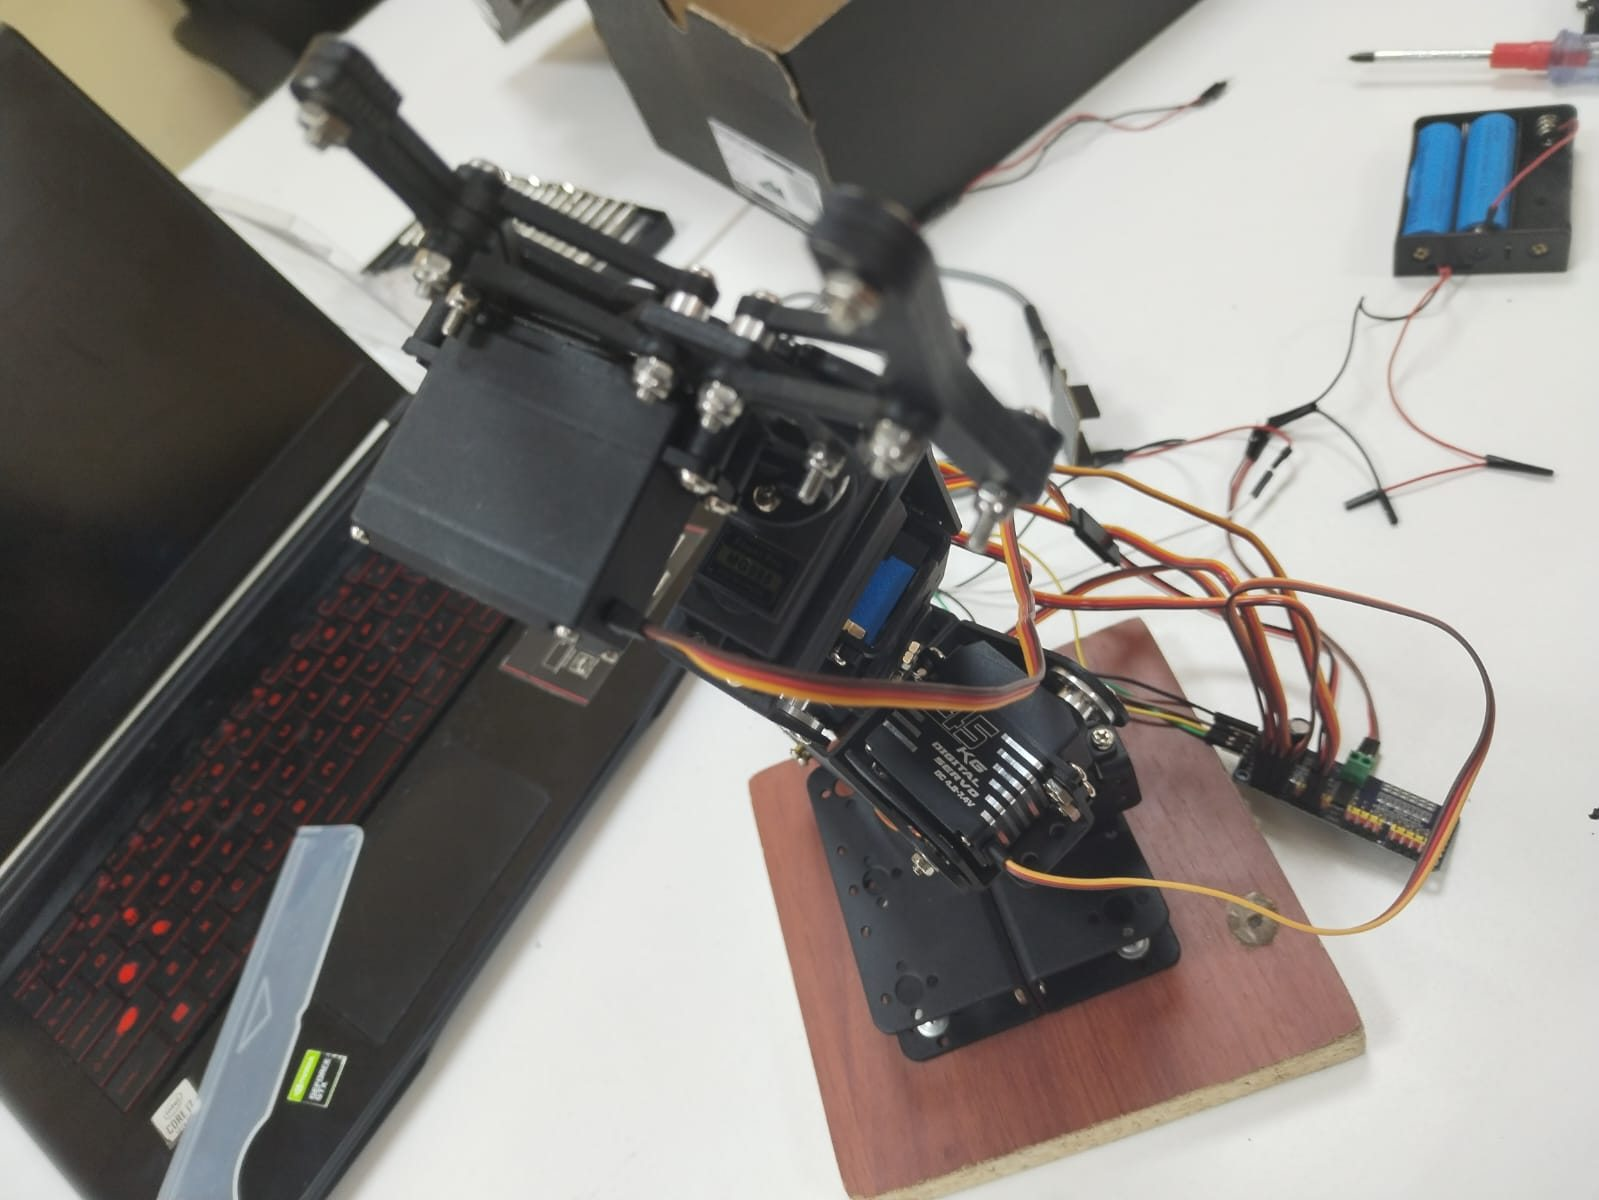
\includegraphics[width=\linewidth,height=7cm,keepaspectratio]{img/evidencia_brazo_articulaciones_closeup.jpg}
  \caption{Detalle de los soportes y uniones cercanos a la pinza.}
 \end{subfigure}
 \caption{Posturas de referencia para la revisión de alineación y holguras.}
 \label{fig:actualizacion_posturas}
\end{figure}

\begin{figure}[H]
 \centering
 \begin{subfigure}[t]{0.48\textwidth}
  \centering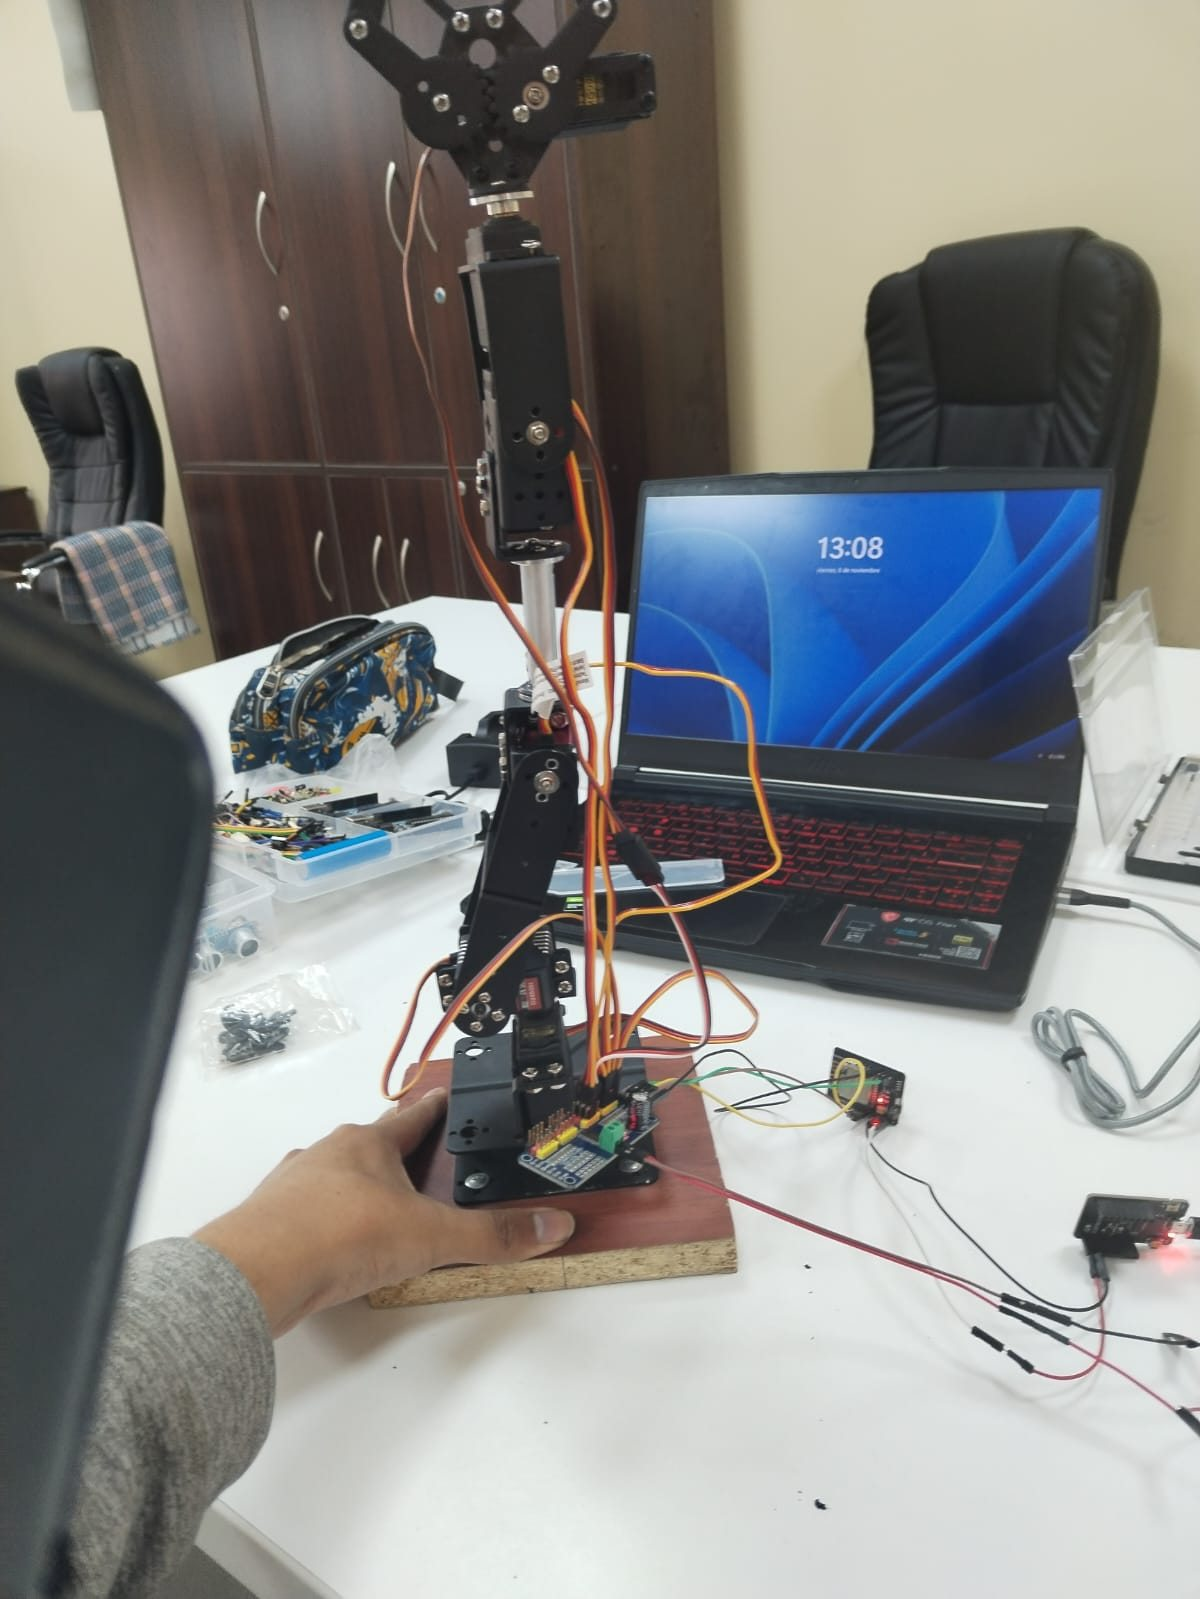
\includegraphics[width=\linewidth,height=7cm,keepaspectratio]{img/evidencia_brazo_estabilidad_base.jpg}
  \caption{Sujeción manual del conjunto a su base.}
 \end{subfigure}\hfill
 \begin{subfigure}[t]{0.48\textwidth}
  \centering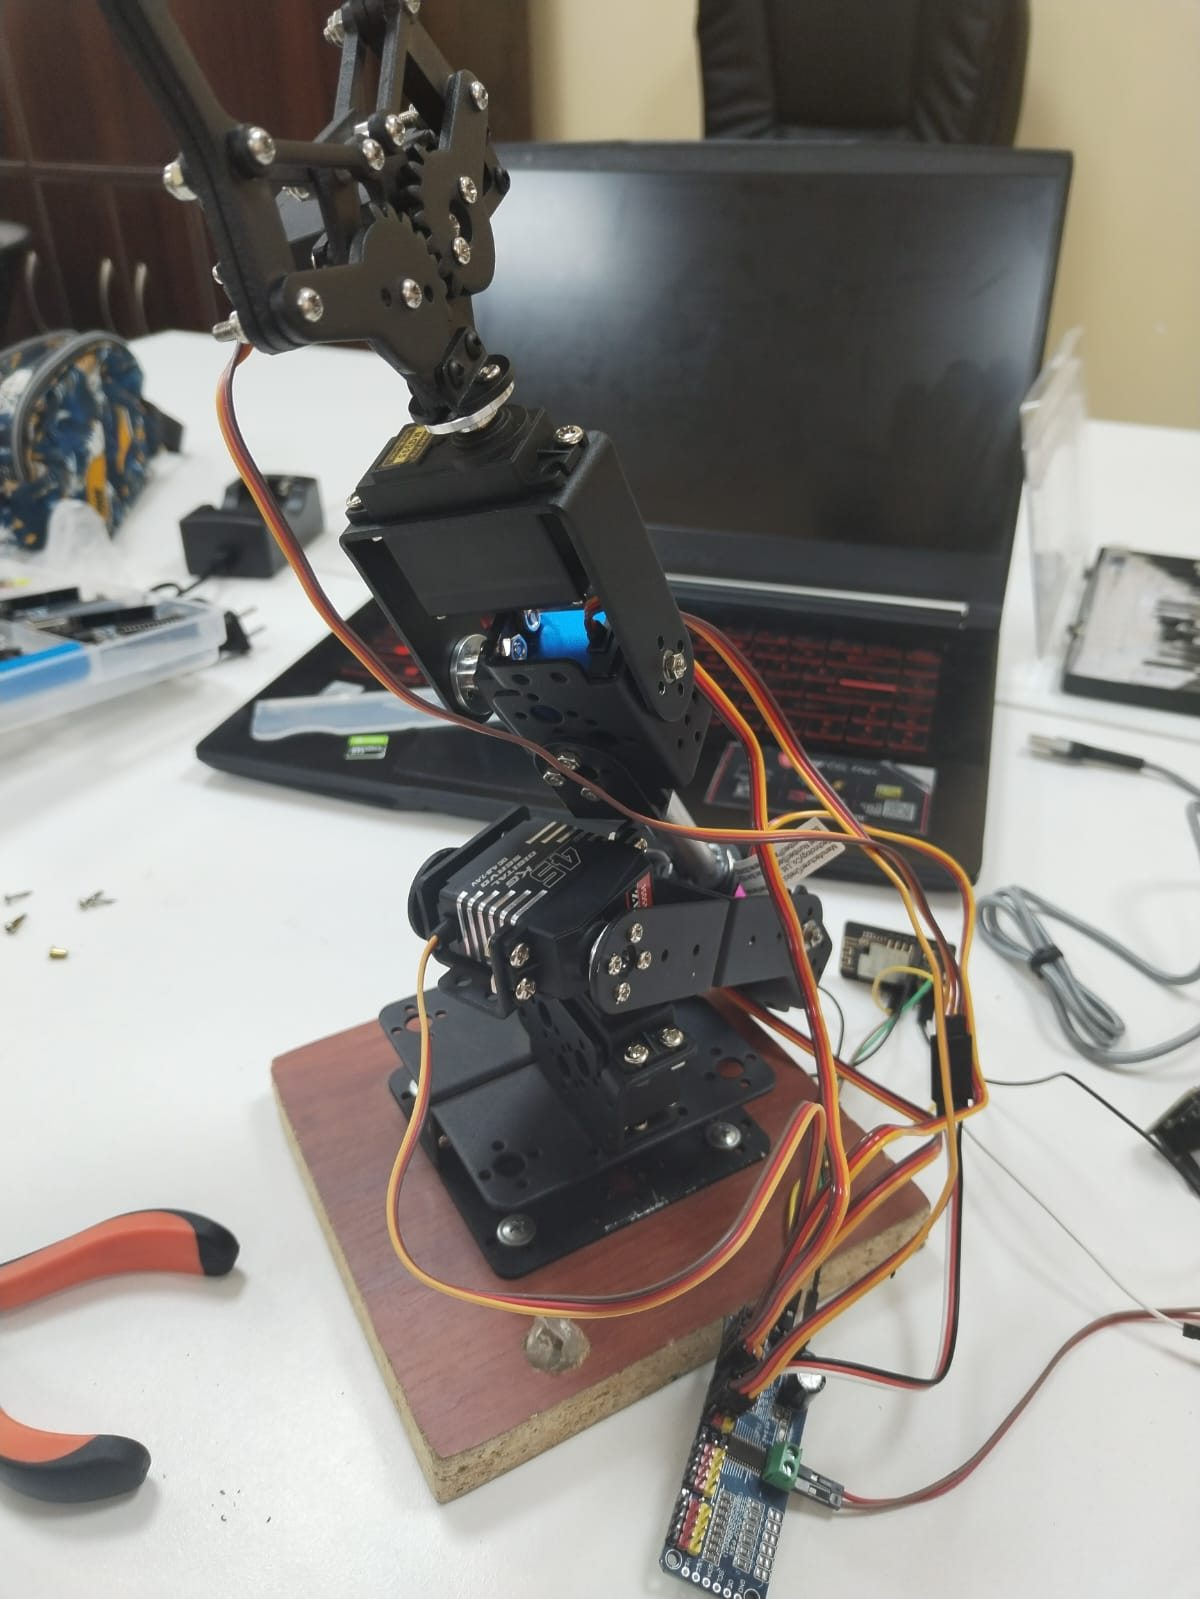
\includegraphics[width=\linewidth,height=7cm,keepaspectratio]{img/evidencia_brazo_soportes_mecanicos.jpg}
  \caption{Vista cercana de servomotores, soportes y tornillería.}
 \end{subfigure}
 \caption{Inspección mecánica de las articulaciones y la plataforma soporte.}
 \label{fig:actualizacion_base}
\end{figure}

\subsection{Integración del ESP32 y del controlador PCA9685}
En las imágenes se reconoce el módulo PCA9685, cuyas cabeceras distribuyen las señales de control hacia los servomotores. El controlador recibe las órdenes por el bus $I^2C$ y genera las señales PWM independientemente del procesador. La fotografía del cableado permite observar conexiones entre módulos, aunque no basta para certificar continuidad, polaridad o asignación exacta de cada conductor. En el firmware del repositorio se configuran de forma nominal SDA en GPIO 13, SCL en GPIO 14 y dirección $I^2C$ \texttt{0x40}; estos valores deben contrastarse con el montaje realmente utilizado.

\begin{figure}[H]
 \centering
 \begin{subfigure}[t]{0.48\textwidth}
  \centering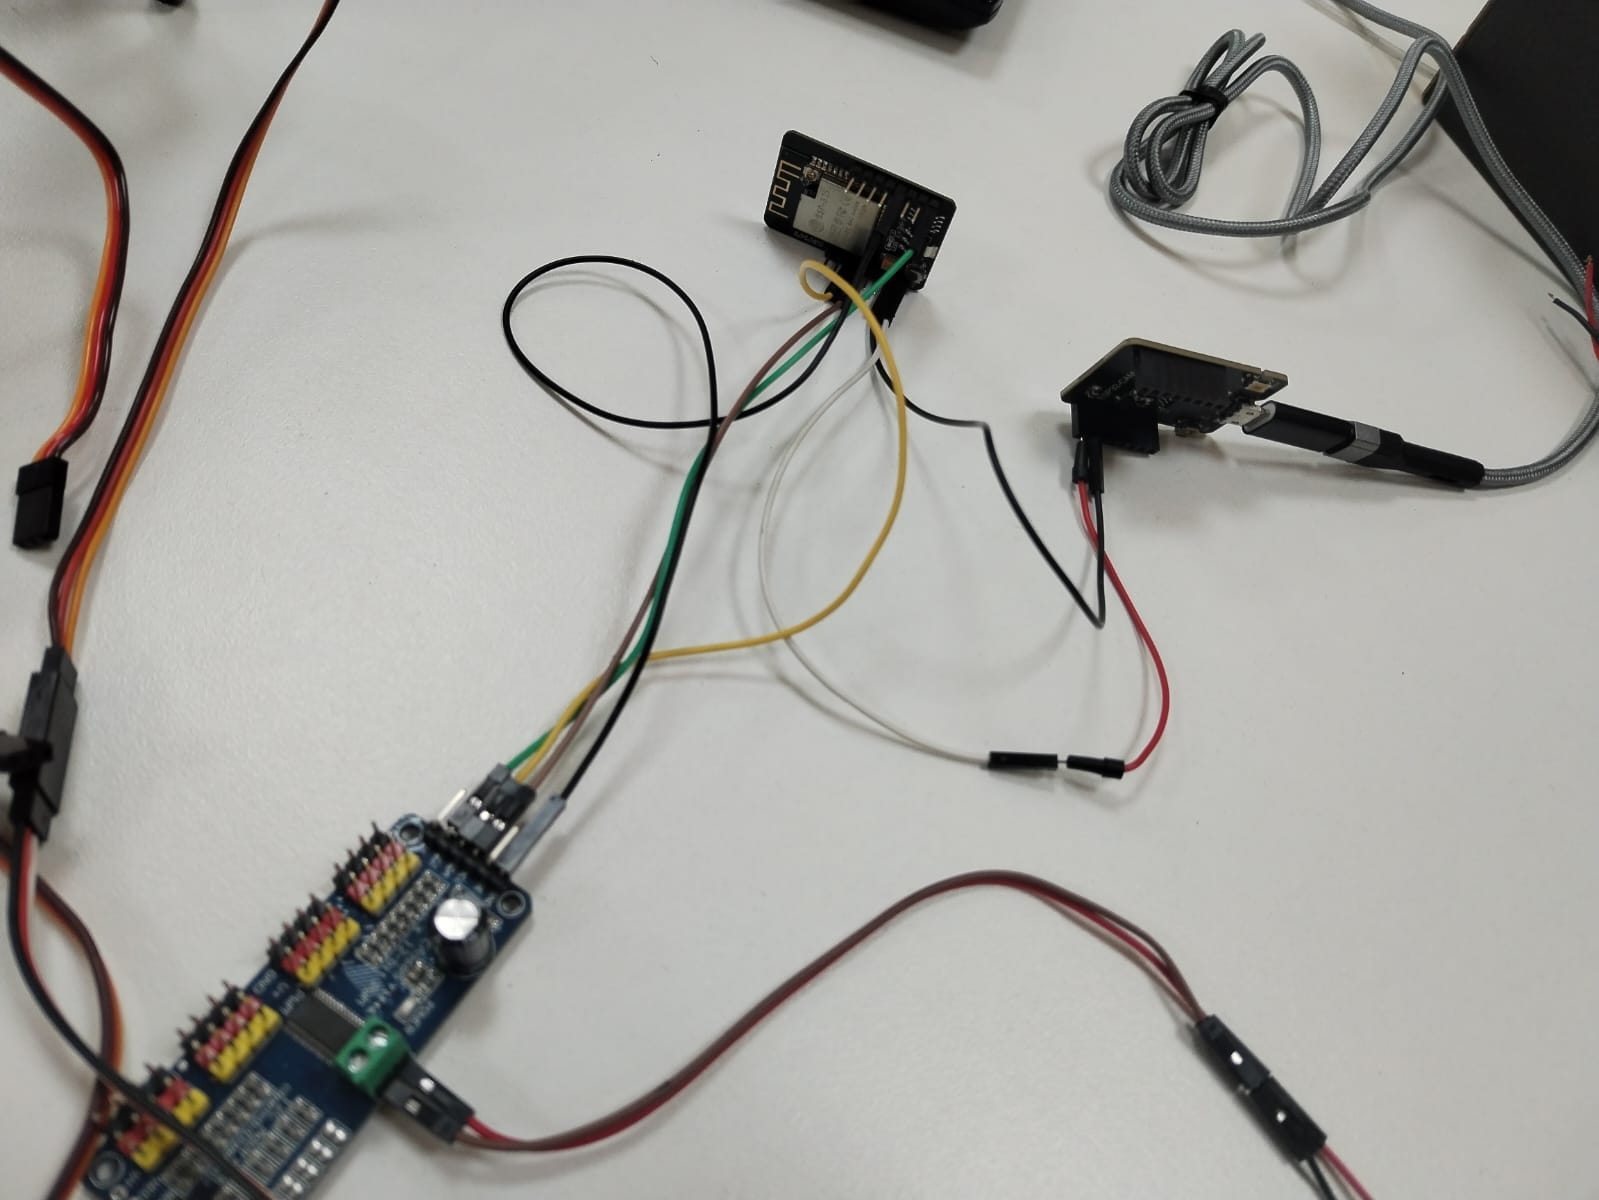
\includegraphics[width=\linewidth,height=7cm,keepaspectratio]{img/evidencia_esp32_pca9685_cableado.jpg}
  \caption{Módulos electrónicos y conductores de interconexión.}
 \end{subfigure}\hfill
 \begin{subfigure}[t]{0.48\textwidth}
  \centering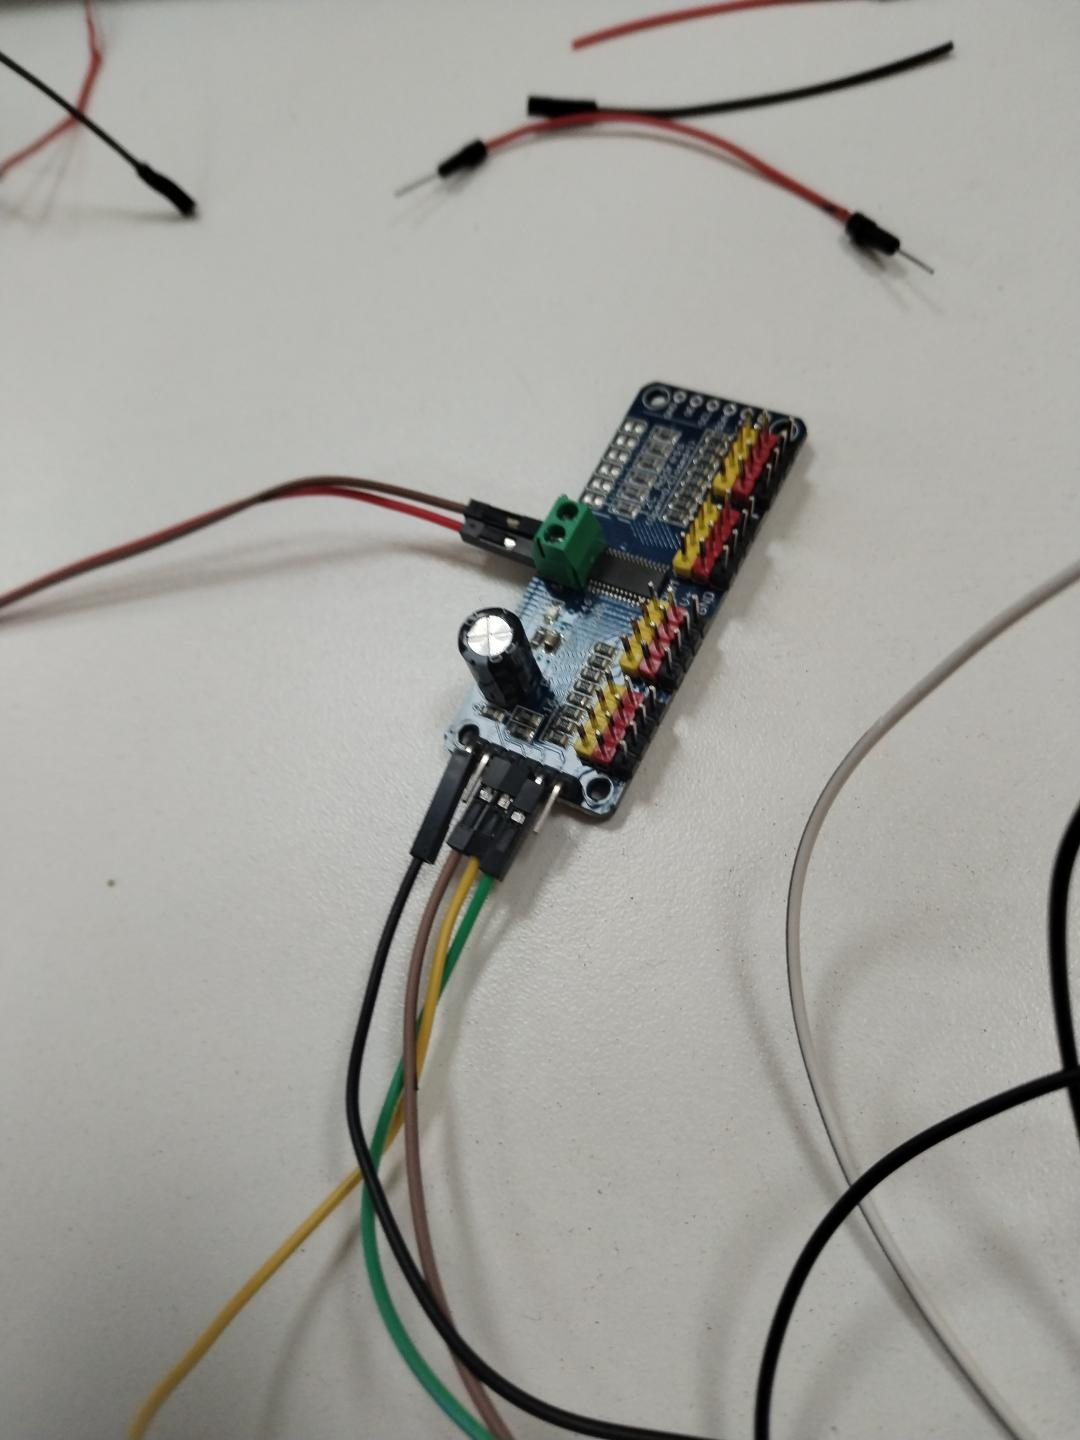
\includegraphics[width=\linewidth,height=7cm,keepaspectratio]{img/evidencia_pca9685_detalle.jpg}
  \caption{Vista cercana del PCA9685 y su bornera.}
 \end{subfigure}
 \caption{Evidencia de avance en la integración del sistema de control electrónico.}
 \label{fig:actualizacion_pca}
\end{figure}

Para validar esta etapa se propone realizar una lectura del bus $I^2C$ con el programa de escaneo del repositorio y registrar el resultado en el monitor serie. Una detección de \texttt{0x40} demostraría comunicación digital con el controlador, pero no permitiría concluir por sí sola que los servomotores estén bien alimentados o que su movimiento sea seguro.

\subsection{Revisión de fuentes de alimentación y baterías}
Las evidencias incluyen un portapilas con dos celdas cilíndricas y una batería plana recargable. Su presencia documenta la evaluación de alternativas de alimentación; no se puede establecer a partir de las fotografías cuál fue conectada durante cada ensayo ni verificar su tensión, capacidad efectiva o corriente disponible. Antes de suministrar energía al riel de servomotores se debe medir la salida con un multímetro y comprobar que la tensión resultante no supere la admisible para el conjunto de servos empleado. No debe asumirse que dos celdas tienen una tensión determinada sin conocer su conexión serie/paralelo y su estado de carga.

\begin{figure}[H]
 \centering
 \begin{subfigure}[t]{0.48\textwidth}
  \centering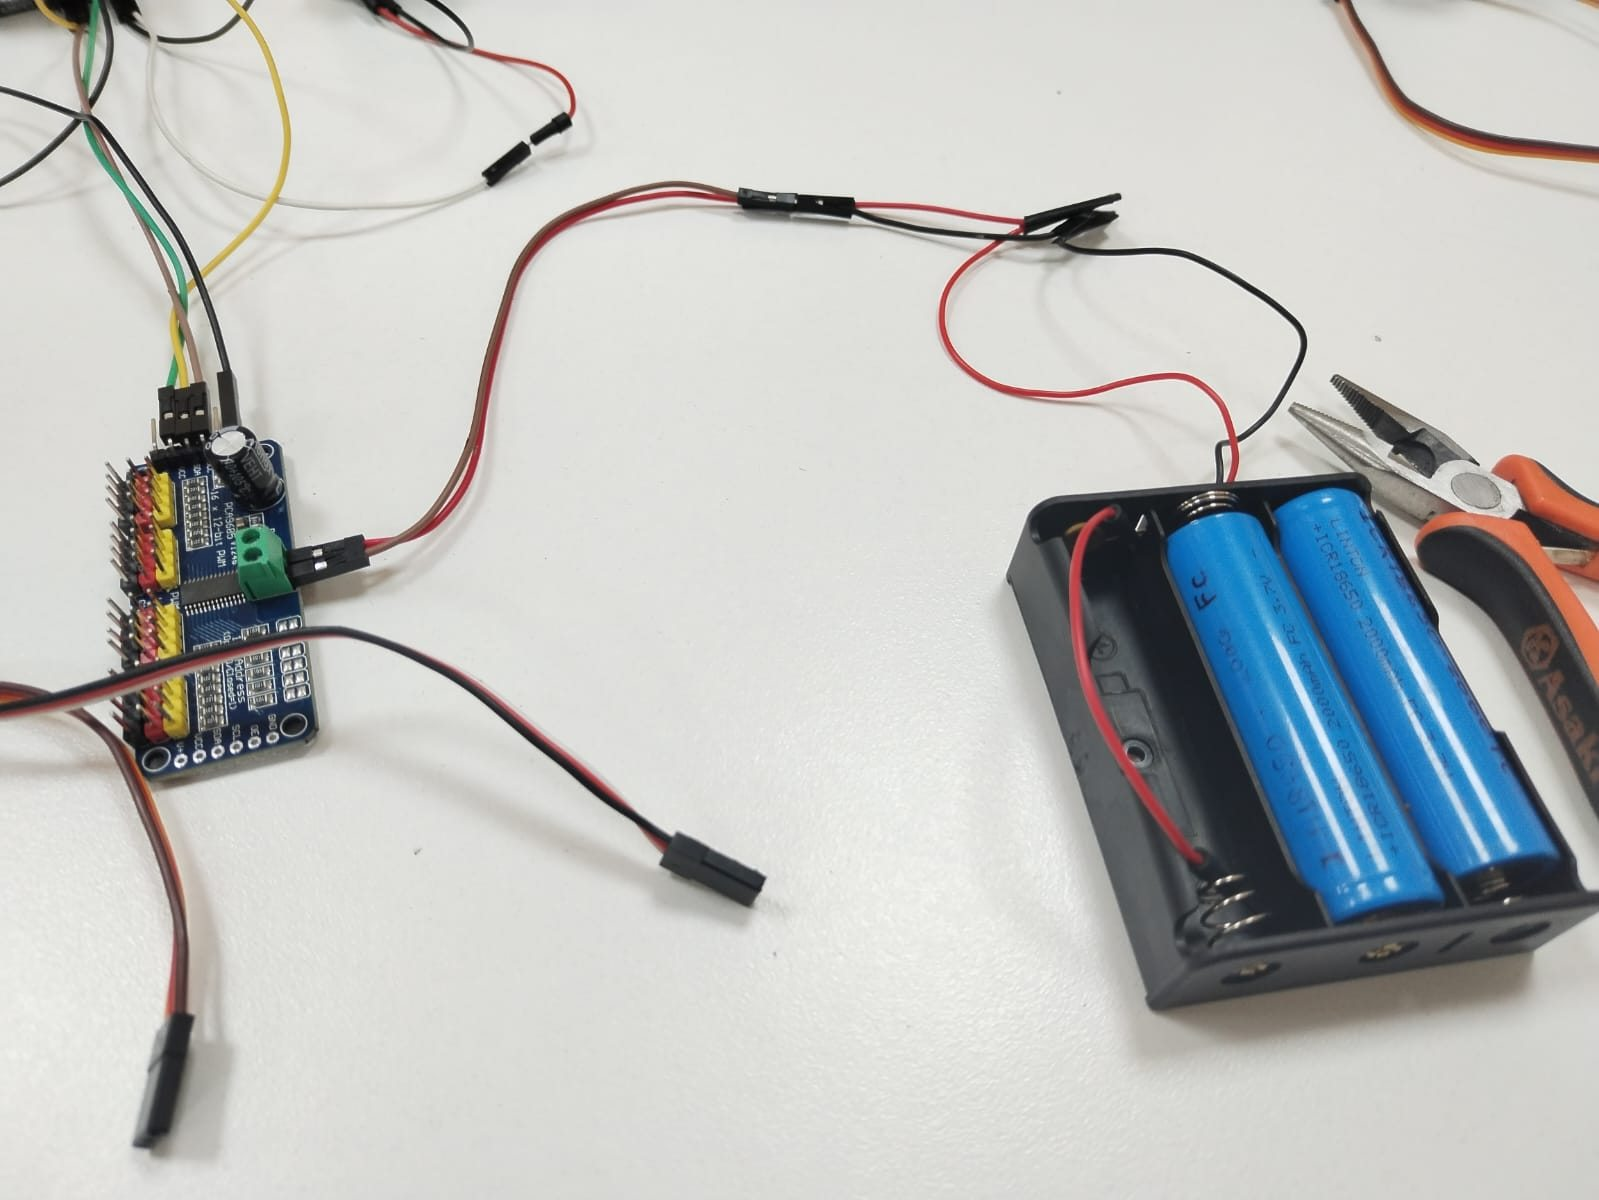
\includegraphics[width=\linewidth,height=7cm,keepaspectratio]{img/evidencia_portapilas_pca9685.jpg}
  \caption{Portapilas de dos celdas junto al PCA9685.}
 \end{subfigure}\hfill
 \begin{subfigure}[t]{0.48\textwidth}
  \centering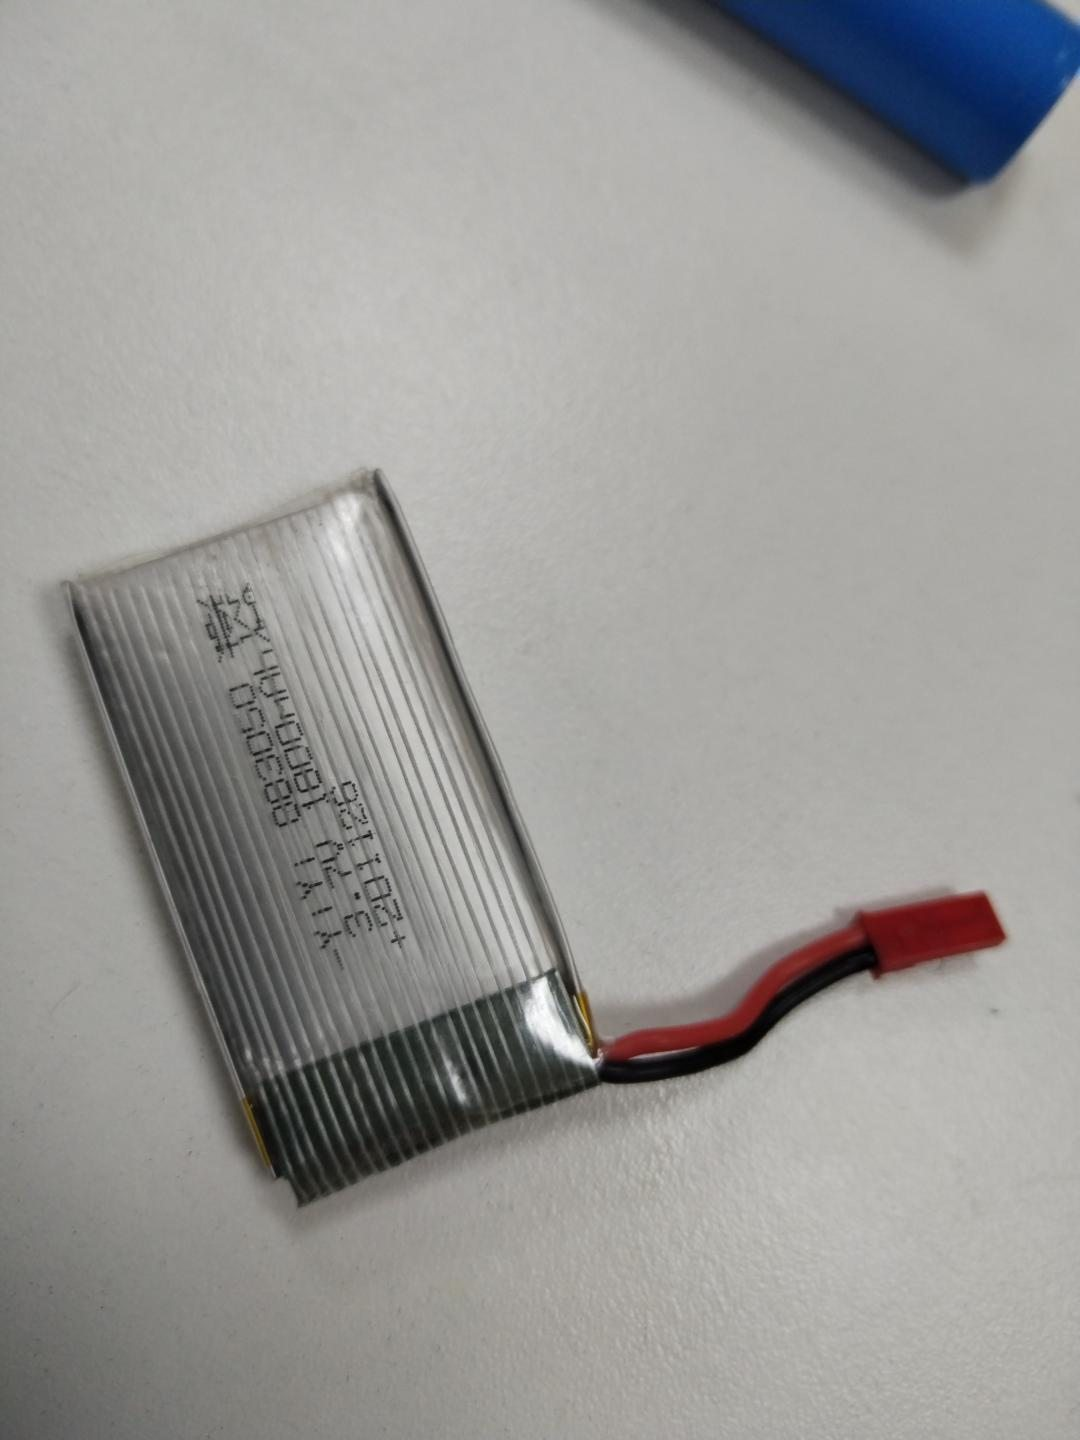
\includegraphics[width=\linewidth,height=7cm,keepaspectratio]{img/evidencia_bateria_lipo.jpg}
  \caption{Batería recargable plana observada en el laboratorio.}
 \end{subfigure}
 \caption{Alternativas de alimentación fotografiadas durante la integración.}
 \label{fig:actualizacion_fuentes}
\end{figure}

Es imprescindible separar la alimentación lógica del ESP32 de la alimentación de potencia de los actuadores, mantener una referencia GND común donde corresponda y utilizar una fuente con corriente suficiente para los picos de los servos. Las baterías de litio requieren protección adecuada contra cortocircuitos, sobrecorriente y descarga excesiva. La desactivación PWM por software no equivale a un interruptor físico de emergencia.

\subsection{Verificación de comunicación local mediante Wi-Fi}
En una captura previa, el teléfono aparece conectado a una red identificada como \texttt{FRANKI-HE}, sin acceso a Internet. Esto es compatible con un funcionamiento en red local: un punto de acceso puede permitir comunicación con dispositivos conectados sin ofrecer salida a Internet. Una segunda captura muestra la dirección privada \texttt{192.168.4.1} con una interfaz web de configuración de la cámara OV2640, incluyendo resolución QVGA (320$\times$240) y controles de exposición, brillo y contraste. Esta captura es evidencia del acceso HTTP a una interfaz de cámara en la red local, aunque no prueba el funcionamiento del panel de servos documentado en el código principal. También debe señalarse que el SSID observado, \texttt{FRANKI-HE}, no coincide con el SSID \texttt{Brazo-ESP32CAM} configurado en la versión revisada de \texttt{brazoR.ino}, por lo que podría corresponder a otra configuración o versión de prueba.

\begin{figure}[H]
 \centering
 \begin{subfigure}[t]{0.48\textwidth}
  \centering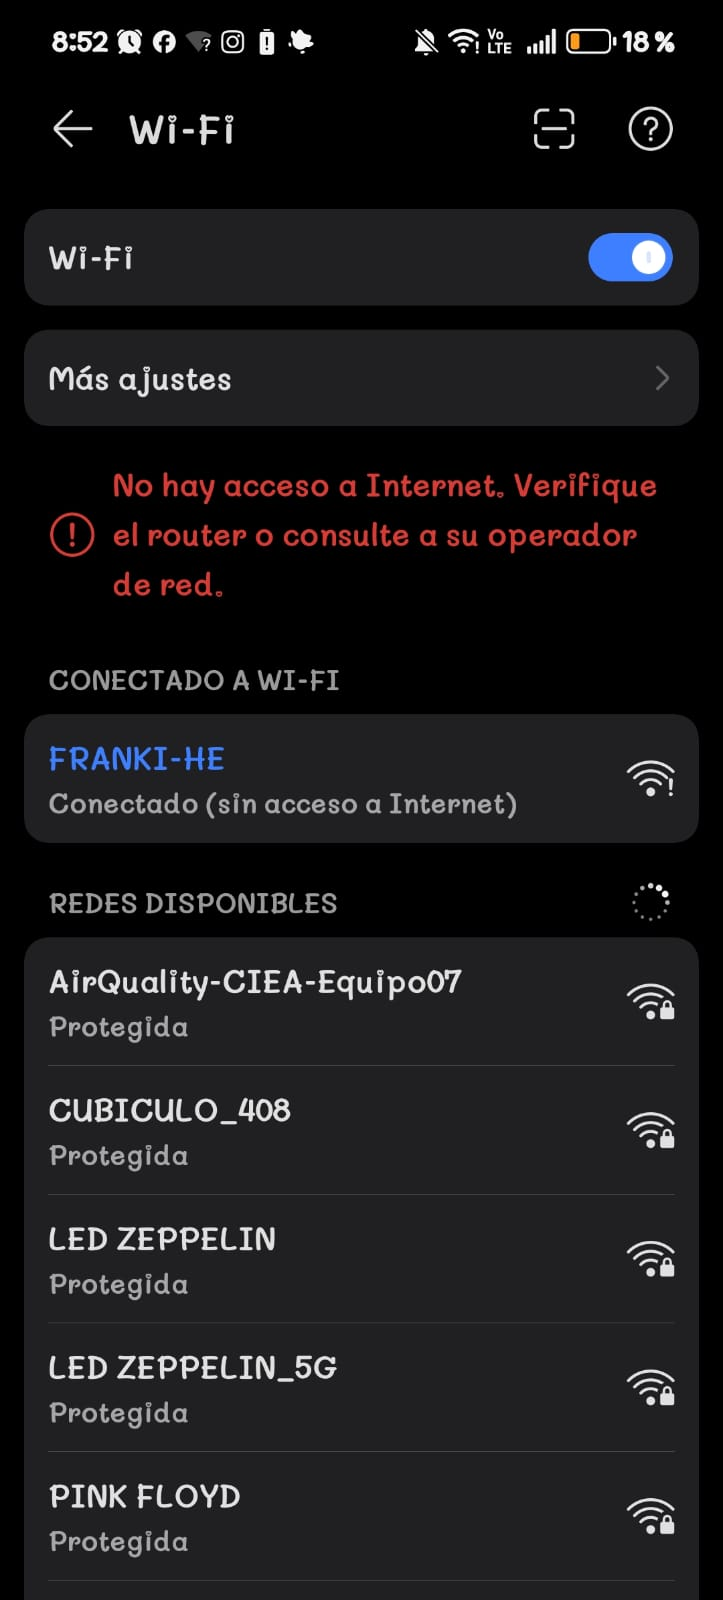
\includegraphics[width=\linewidth,height=9cm,keepaspectratio]{img/evidencia_wifi_red_local.png}
  \caption{Red local \texttt{FRANKI-HE} conectada.}
 \end{subfigure}\hfill
 \begin{subfigure}[t]{0.48\textwidth}
  \centering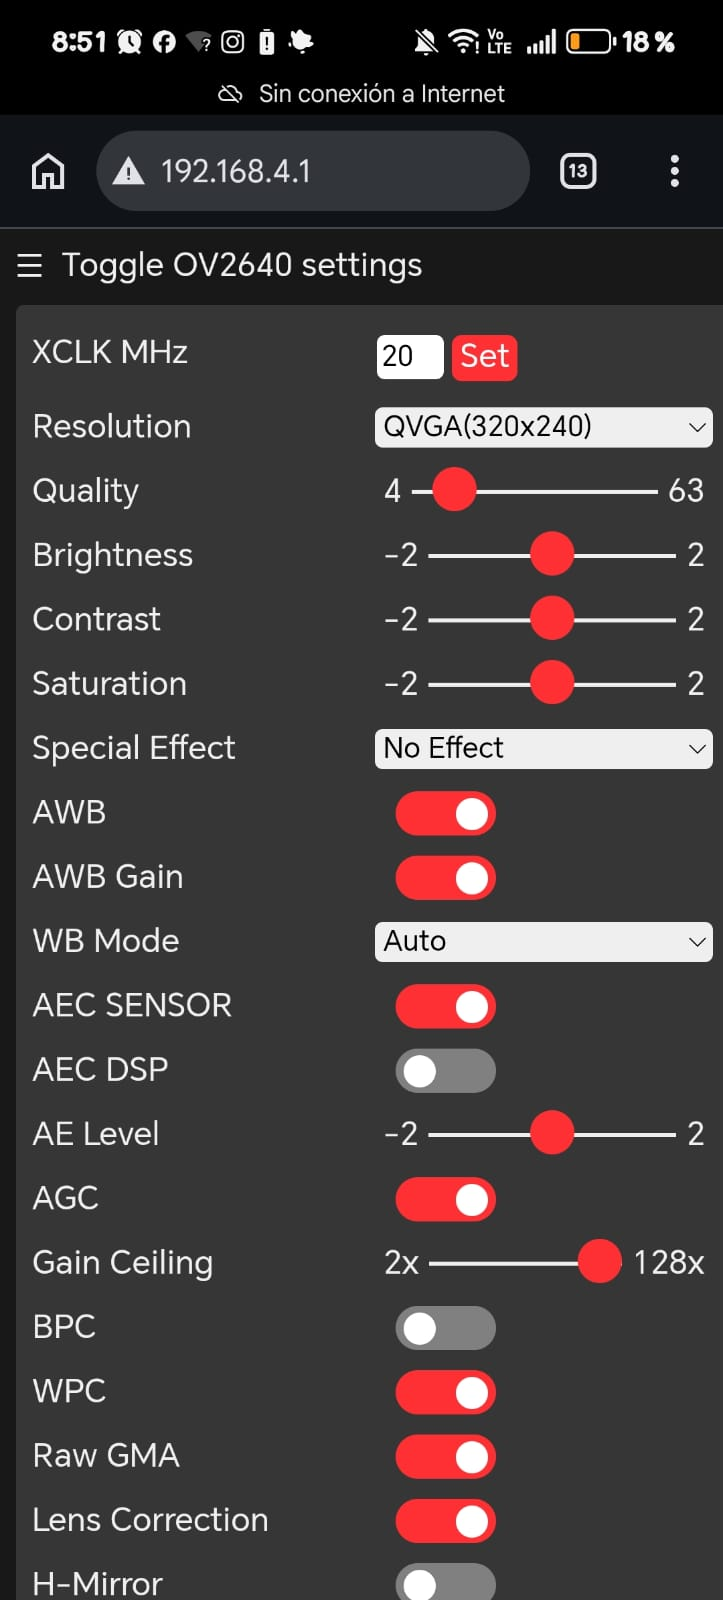
\includegraphics[width=\linewidth,height=9cm,keepaspectratio]{img/evidencia_wifi_panel_ov2640.png}
  \caption{Interfaz OV2640 en \texttt{192.168.4.1}.}
 \end{subfigure}
 \caption{Evidencias de comunicación inalámbrica y acceso web desde un dispositivo móvil.}
 \label{fig:actualizacion_wifi}
\end{figure}

\subsection{Procedimiento de calibración y comprobaciones pendientes}
Para pasar del ensamblaje observado a una calibración verificable se propone: (i) desenergizar y asegurar mecánicamente las uniones; (ii) confirmar el apriete de los servocuernos y la ausencia de holguras; (iii) alimentar un solo servo con una fuente medida y adecuada; (iv) comprobar el centro nominal de $90^\circ$ antes de fijar el eslabón; (v) recorrer gradualmente los límites evitando topes; y (vi) repetir el procedimiento articulación por articulación. El programa del repositorio utiliza límites nominales de $30^\circ$ a $150^\circ$ y debe ajustarse según el espacio mecánico real.

\begin{table}[H]
\centering\small
\caption{Registro de verificaciones y estado de evidencia disponible}
\label{tab:actualizacion_verificaciones}
\begin{tabularx}{\textwidth}{p{4.0cm} X p{3.2cm}}
\toprule
\textbf{Elemento} & \textbf{Evidencia o criterio} & \textbf{Estado documentado}\\
\midrule
Montaje de eslabones & Fotografías del brazo en varias posturas. & Observado\\
Controlador PCA9685 & Fotografías del módulo y del cableado. & Montaje observado\\
Comunicación Wi-Fi & Capturas de red local e interfaz OV2640. & Acceso web observado\\
Tensión de alimentación & Lectura con multímetro y polaridad. & Sin medida aportada\\
Ángulos reales & Comparación entre orden y medición física. & Sin medida aportada\\
Movimiento de seis servos & Ensayo individual con registro de resultados. & No demostrado por las fotos\\
\bottomrule
\end{tabularx}
\end{table}

\subsection{Balance del avance experimental}
Respecto a la documentación previa, las fotografías aportan evidencia adicional de integración física del brazo, presencia de cableado electrónico, disposición del PCA9685, inspección de alimentaciones y acceso a una interfaz web local. Sin embargo, sería incorrecto transformar estas observaciones en resultados cuantitativos de exactitud o autonomía sin mediciones. Como siguiente etapa se recomienda anexar una tabla con tensión de alimentación en reposo y bajo carga, lectura de corriente, posición angular ordenada y observada para cada articulación, y resultado de las pruebas de comunicación y movimiento.

% Usa paquetes ya presentes en main.tex: graphicx, float, booktabs, tabularx, subcaption.

\section{Actualización experimental: ensamble, conexiones y ajustes del manipulador}
\label{sec:actualizacion_evidencias}

\subsection{Objeto y alcance del registro fotográfico}
Las evidencias recopiladas corresponden a una nueva etapa de integración del brazo robótico articulado. Se observan diferentes configuraciones mecánicas del manipulador, el montaje de un controlador PWM PCA9685, un módulo de la familia ESP32, conexiones mediante cables y elementos empleados para evaluar la alimentación eléctrica. El propósito de esta sección es registrar el progreso físico del prototipo y delimitar las comprobaciones que aún se requieren. Las fotografías son evidencia de montaje, pero no constituyen por sí mismas una medida de precisión, par disponible o estabilidad eléctrica.

\subsection{Progreso del ensamblaje y postura de las articulaciones}
El manipulador conserva una estructura de eslabones rígidos, servomotores montados en soportes metálicos, pinza mecánica y base de madera. Las nuevas imágenes muestran posiciones inclinadas, frontales y casi verticales, útiles para observar la alineación relativa de hombro, codo y muñeca. Estas posiciones sirven como referencia para identificar posibles interferencias, puntos de holgura y distribución del cableado. No se dispone de un registro instrumental de los ángulos reales, por lo que la denominación ``calibración'' se emplea aquí para describir el proceso de ajuste y verificación, no para afirmar que haya concluido.

\begin{figure}[H]
 \centering
 \begin{subfigure}[t]{0.48\textwidth}
  \centering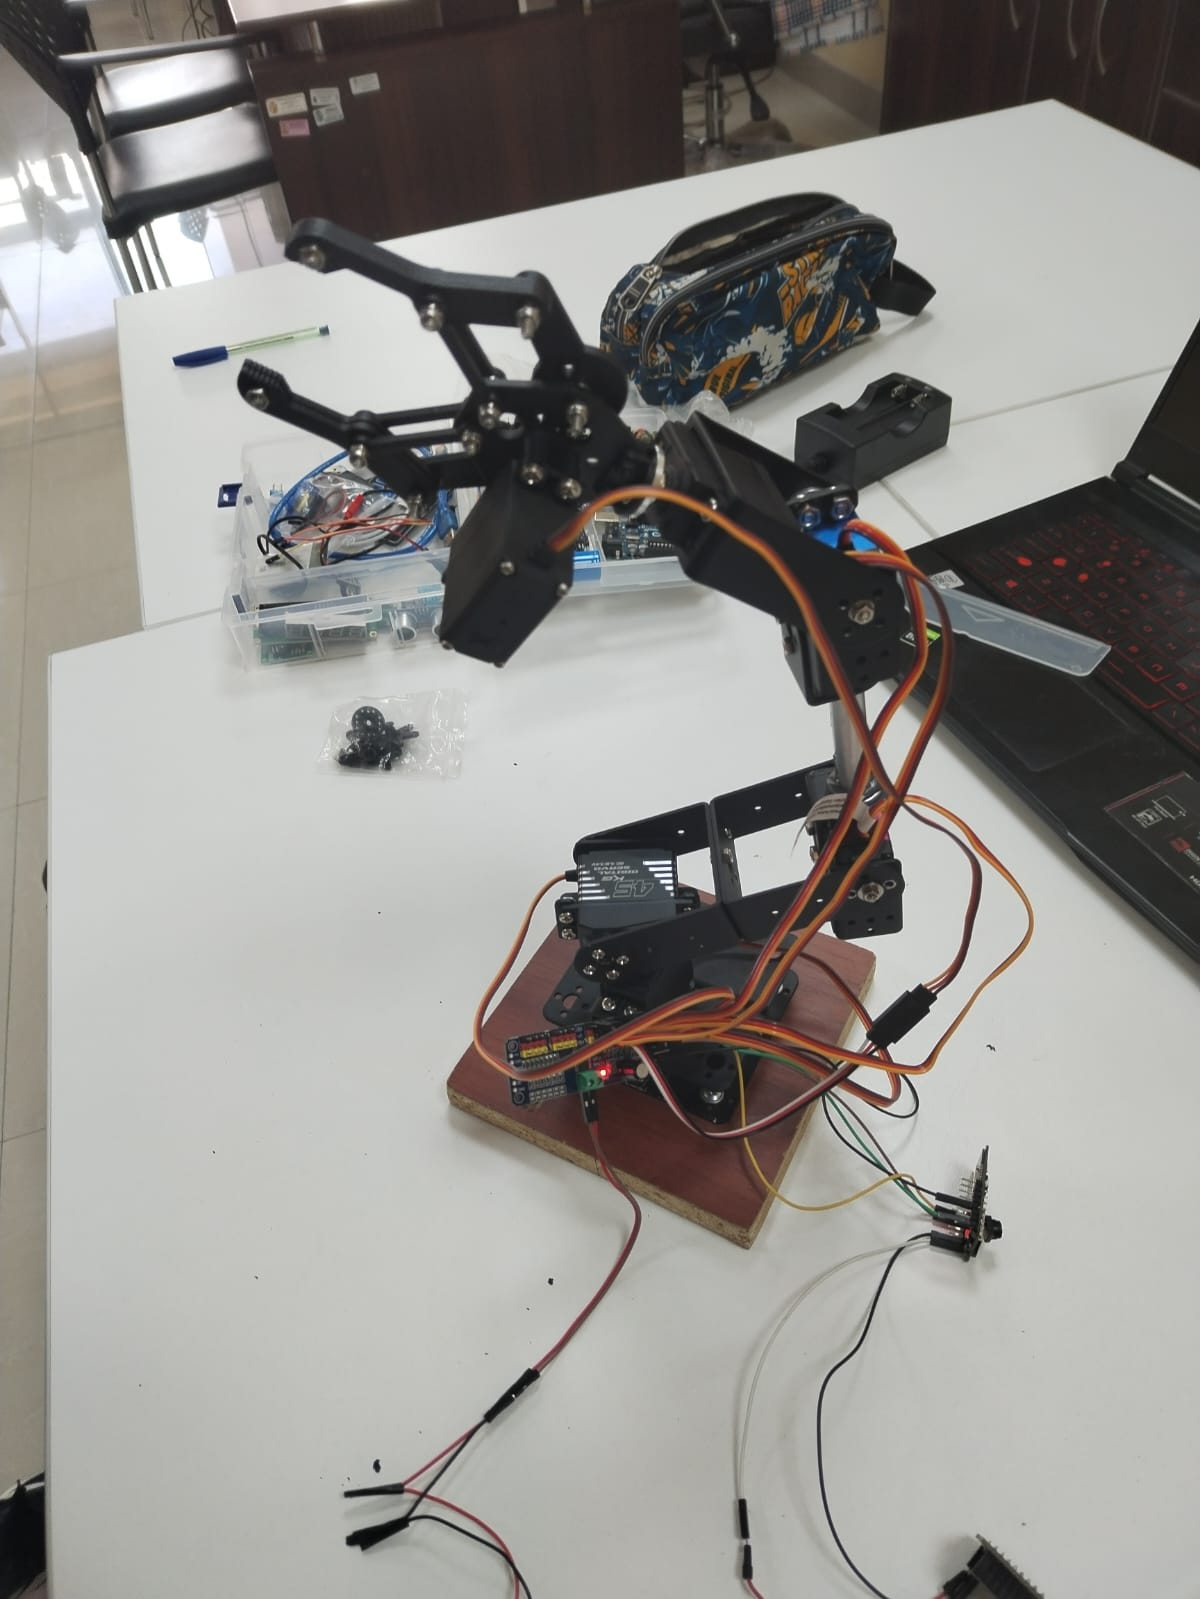
\includegraphics[width=\linewidth,height=7cm,keepaspectratio]{img/evidencia_brazo_integracion_lateral.jpg}
  \caption{Vista lateral durante la integración de la pinza y los eslabones.}
 \end{subfigure}\hfill
 \begin{subfigure}[t]{0.48\textwidth}
  \centering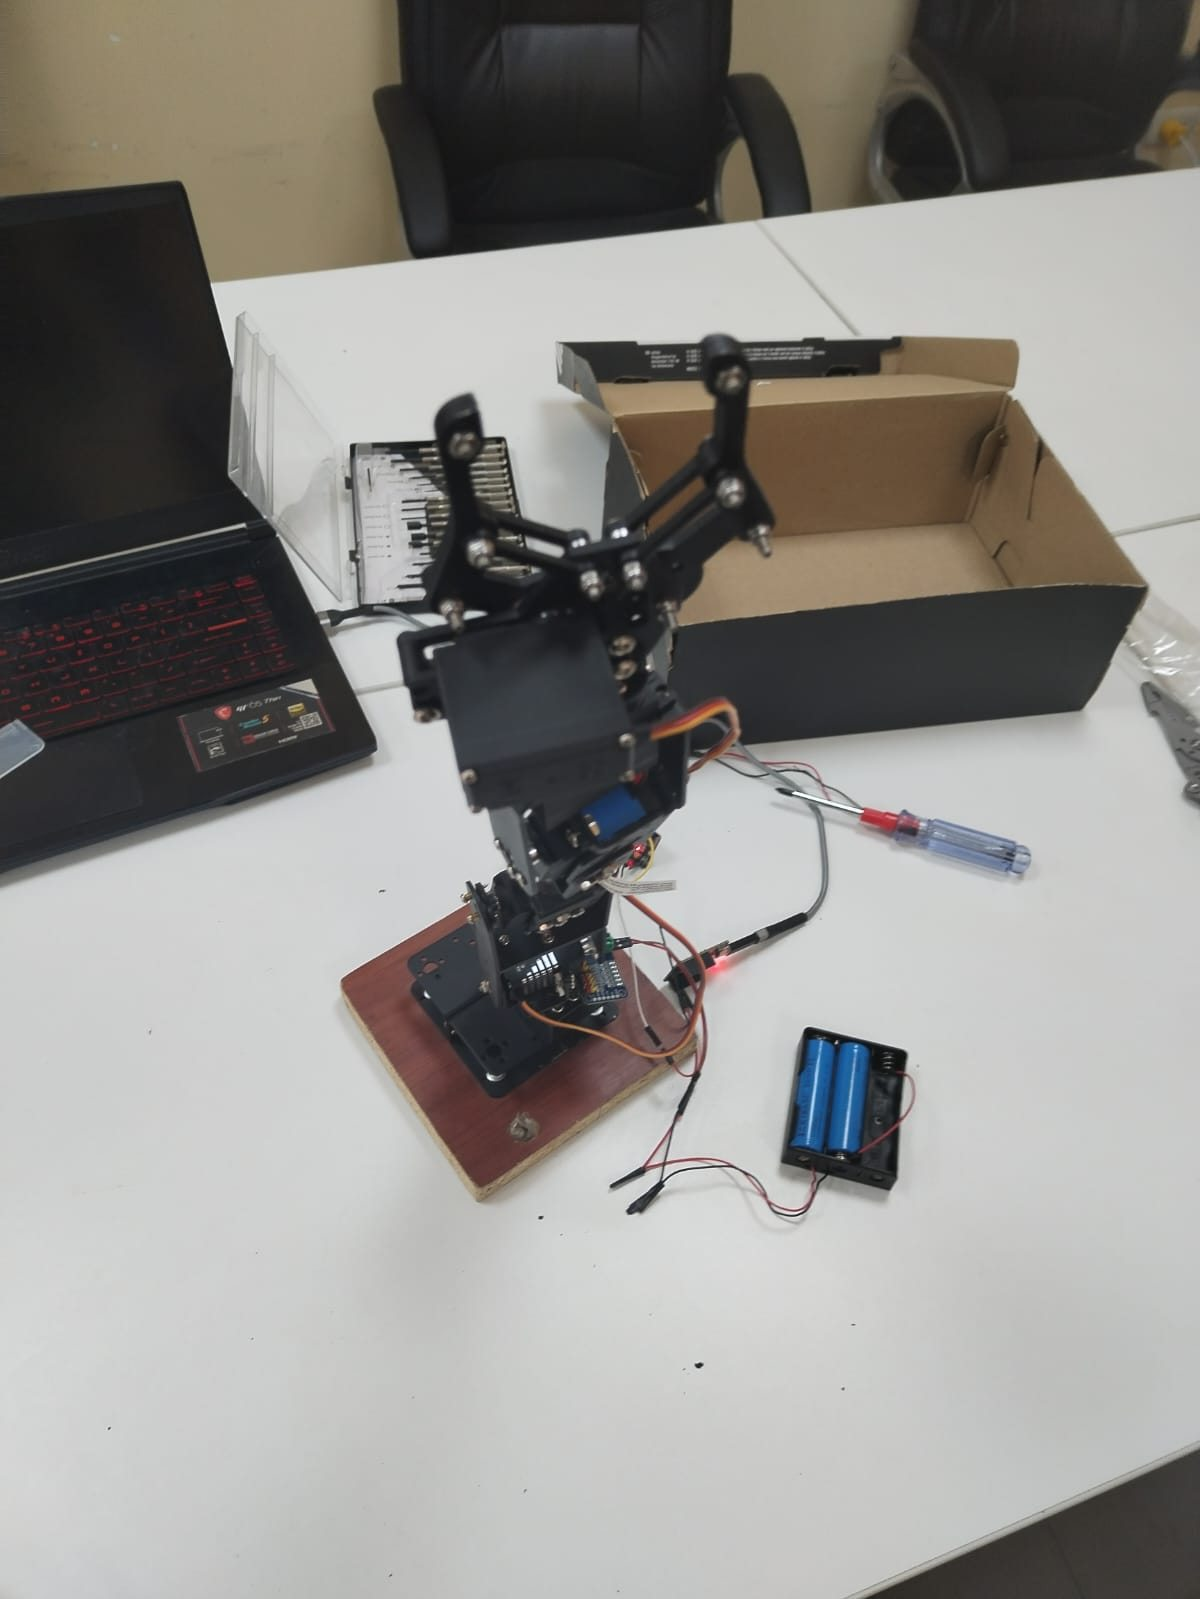
\includegraphics[width=\linewidth,height=7cm,keepaspectratio]{img/evidencia_brazo_vista_frontal.jpg}
  \caption{Vista frontal del conjunto articulado en banco de trabajo.}
 \end{subfigure}
 \caption{Registro del ensamble físico en diferentes orientaciones.}
 \label{fig:actualizacion_ensamble}
\end{figure}

\begin{figure}[H]
 \centering
 \begin{subfigure}[t]{0.48\textwidth}
  \centering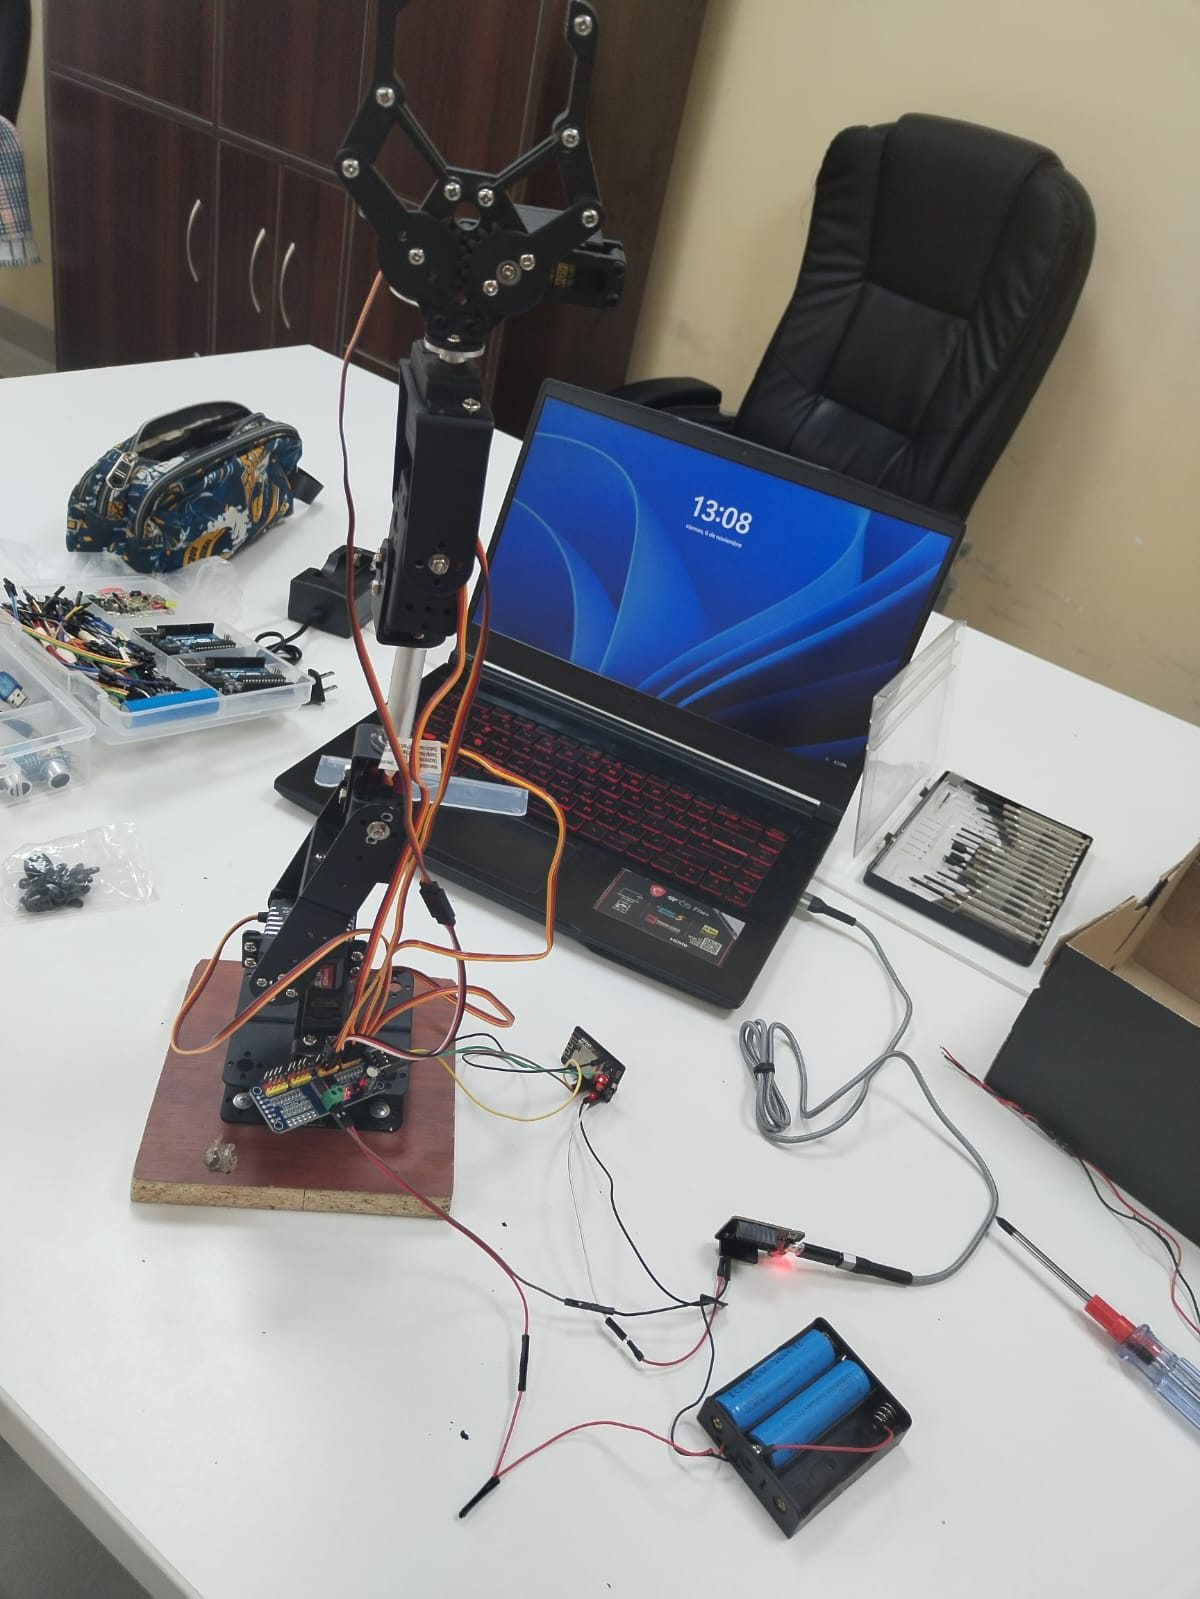
\includegraphics[width=\linewidth,height=7cm,keepaspectratio]{img/evidencia_brazo_postura_vertical.jpg}
  \caption{Prototipo con el efector final elevado.}
 \end{subfigure}\hfill
 \begin{subfigure}[t]{0.48\textwidth}
  \centering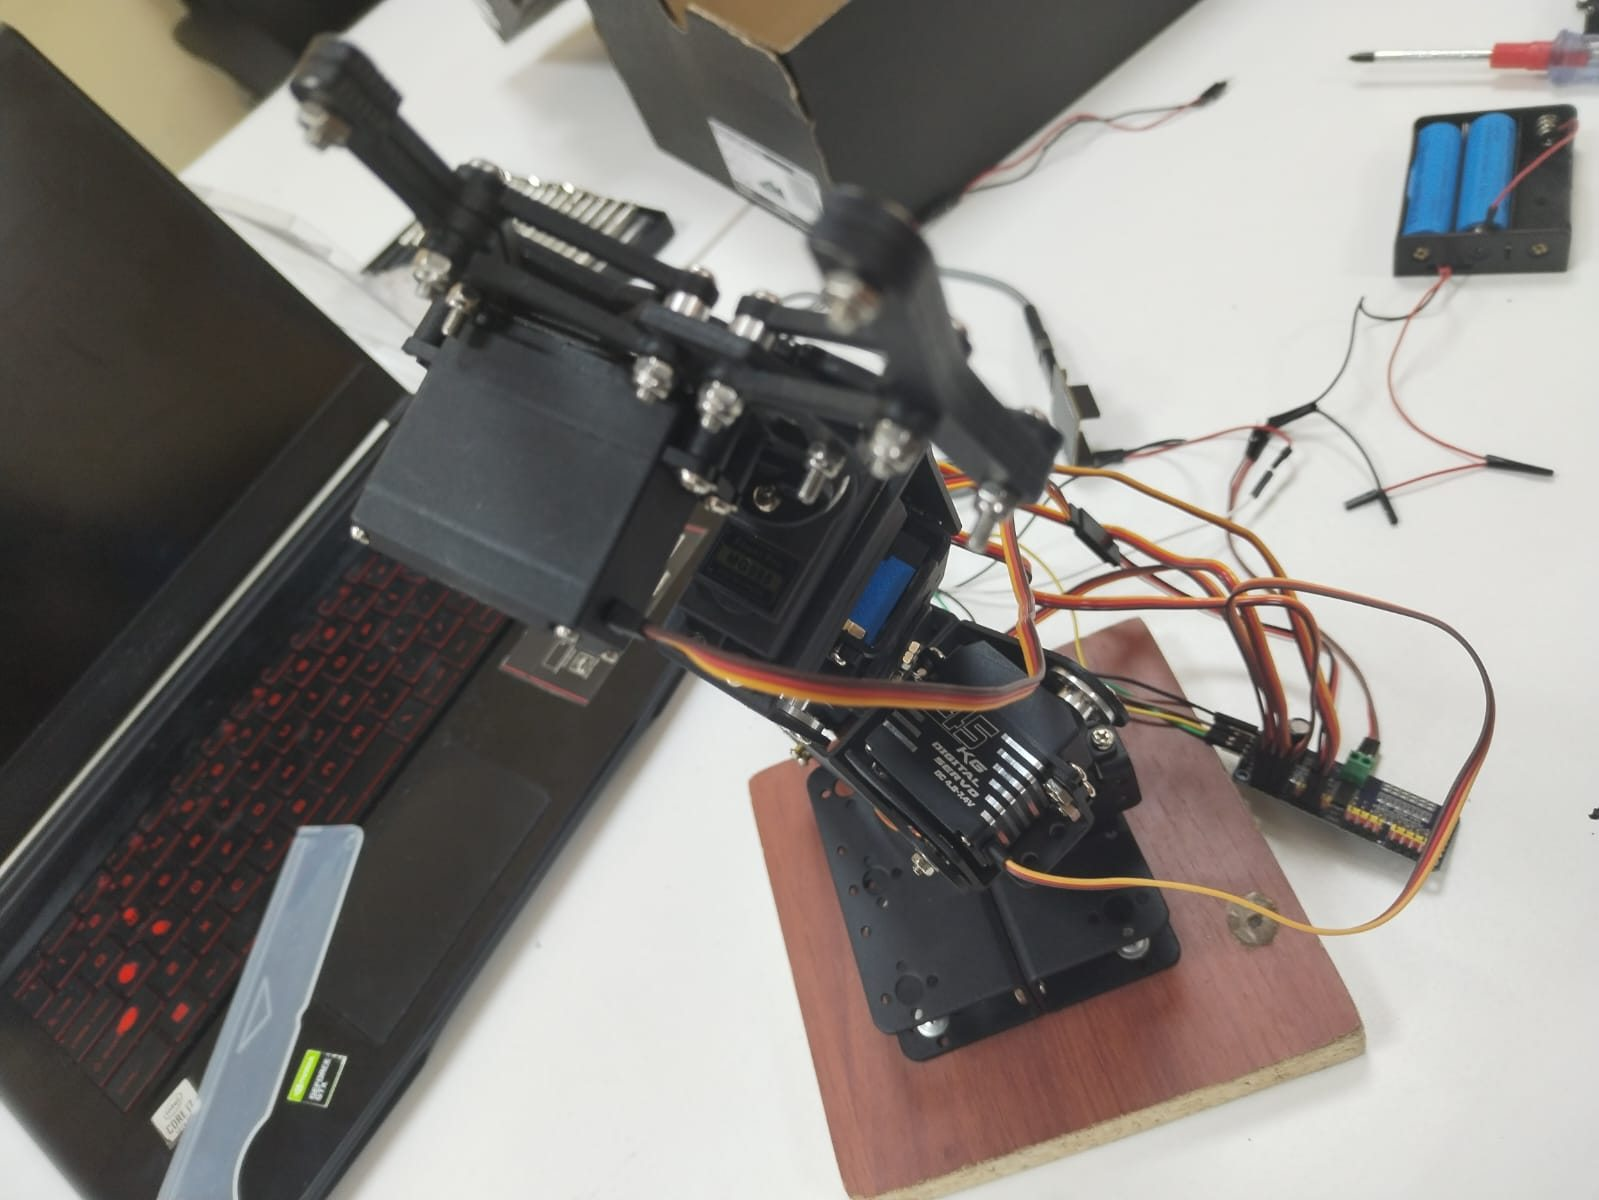
\includegraphics[width=\linewidth,height=7cm,keepaspectratio]{img/evidencia_brazo_articulaciones_closeup.jpg}
  \caption{Detalle de los soportes y uniones cercanos a la pinza.}
 \end{subfigure}
 \caption{Posturas de referencia para la revisión de alineación y holguras.}
 \label{fig:actualizacion_posturas}
\end{figure}

\begin{figure}[H]
 \centering
 \begin{subfigure}[t]{0.48\textwidth}
  \centering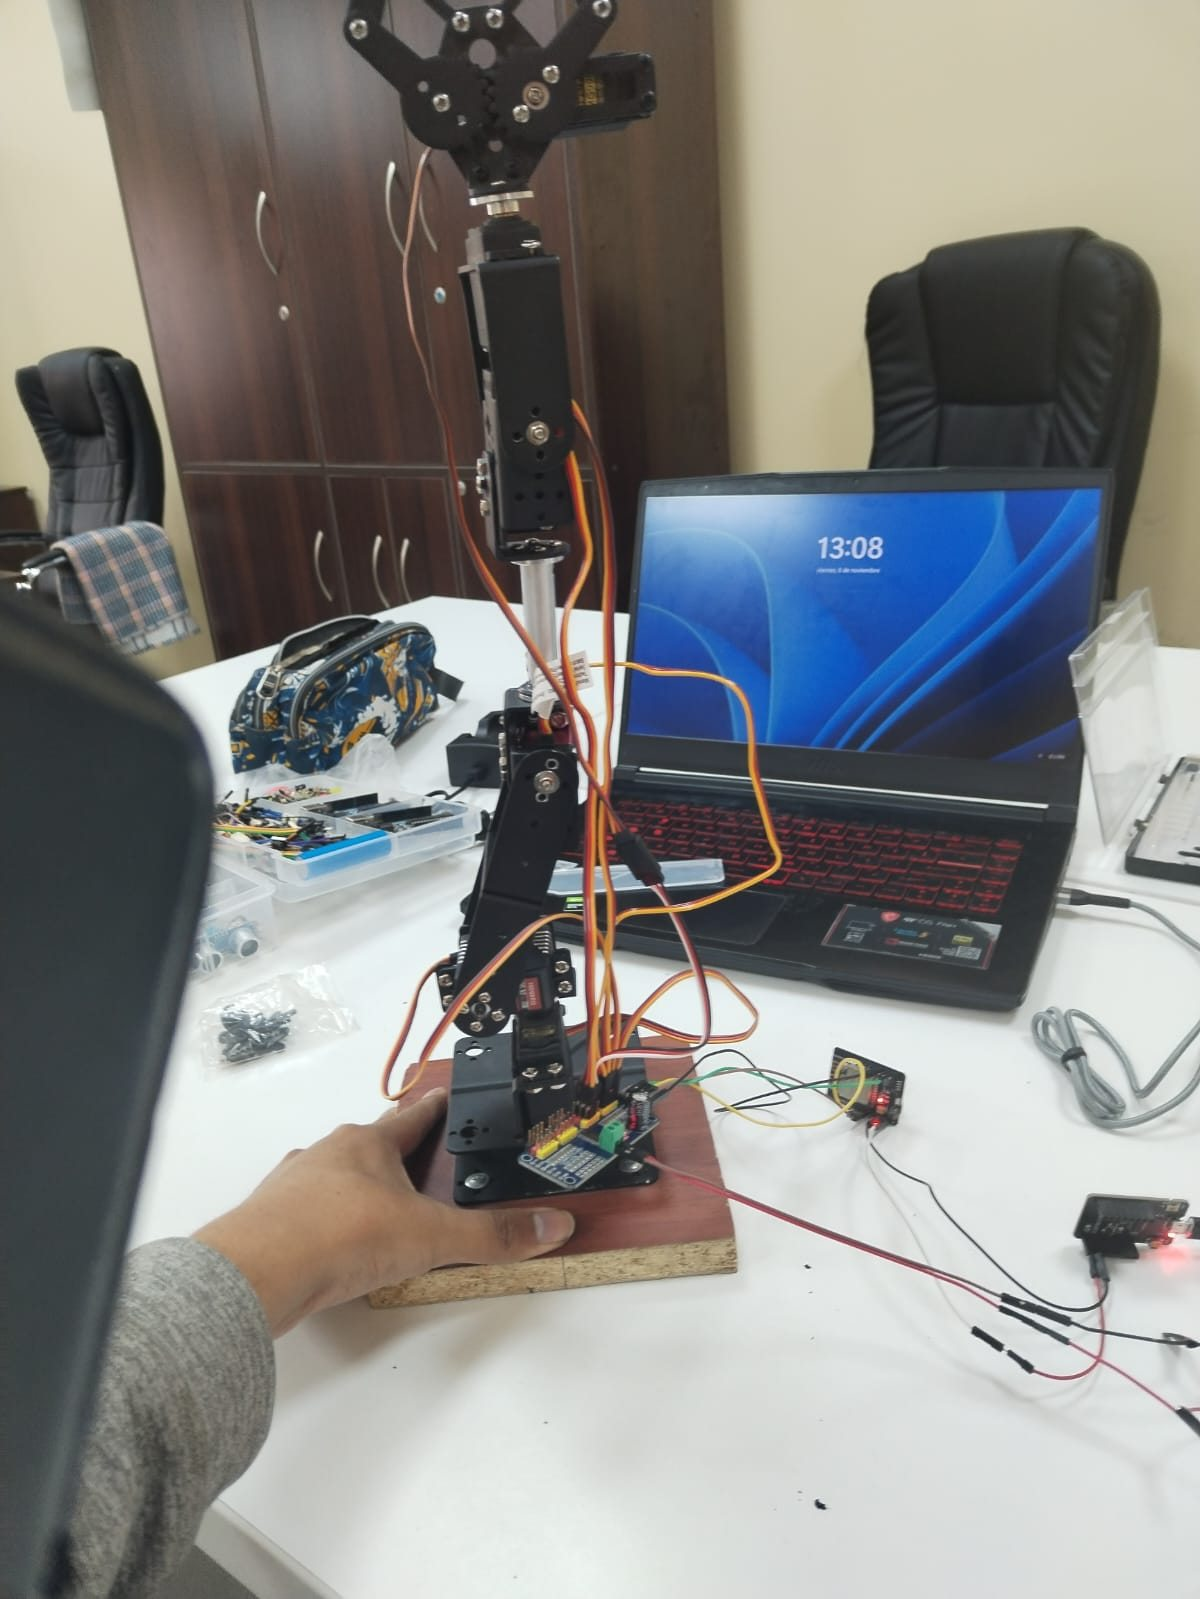
\includegraphics[width=\linewidth,height=7cm,keepaspectratio]{img/evidencia_brazo_estabilidad_base.jpg}
  \caption{Sujeción manual del conjunto a su base.}
 \end{subfigure}\hfill
 \begin{subfigure}[t]{0.48\textwidth}
  \centering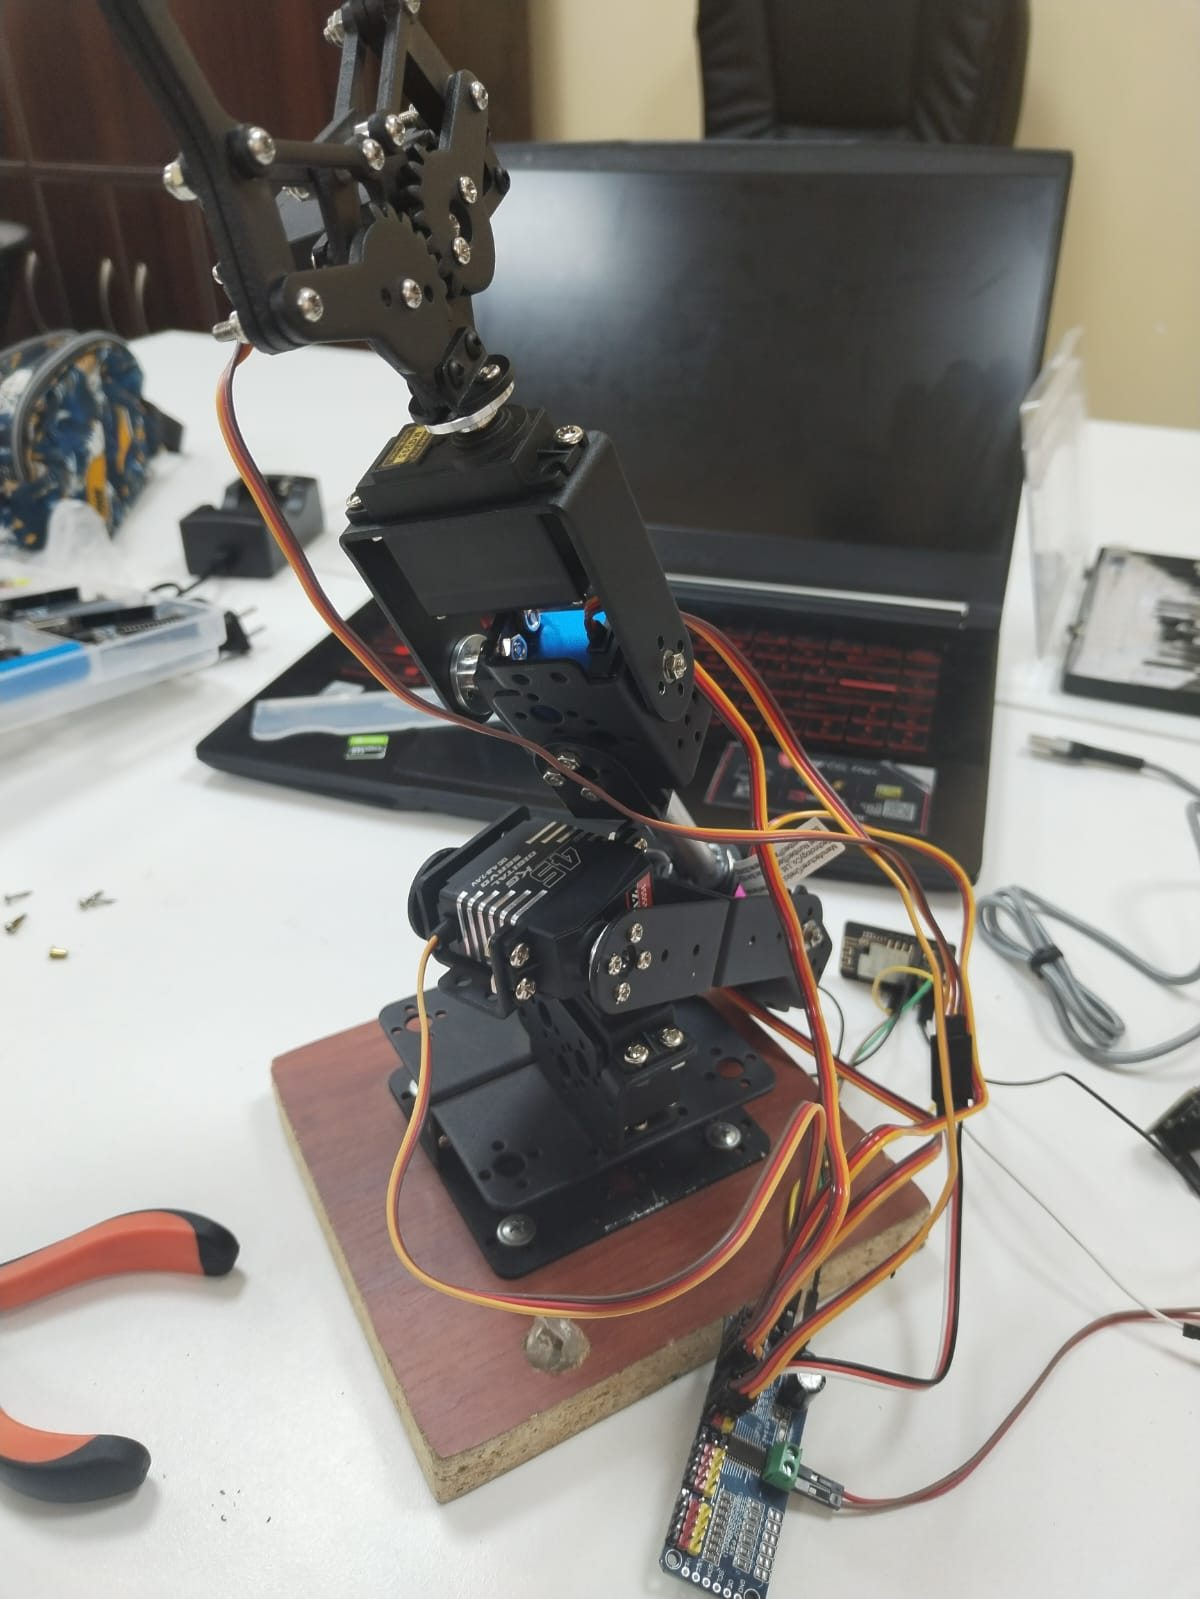
\includegraphics[width=\linewidth,height=7cm,keepaspectratio]{img/evidencia_brazo_soportes_mecanicos.jpg}
  \caption{Vista cercana de servomotores, soportes y tornillería.}
 \end{subfigure}
 \caption{Inspección mecánica de las articulaciones y la plataforma soporte.}
 \label{fig:actualizacion_base}
\end{figure}

\subsection{Integración del ESP32 y del controlador PCA9685}
En las imágenes se reconoce el módulo PCA9685, cuyas cabeceras distribuyen las señales de control hacia los servomotores. El controlador recibe las órdenes por el bus $I^2C$ y genera las señales PWM independientemente del procesador. La fotografía del cableado permite observar conexiones entre módulos, aunque no basta para certificar continuidad, polaridad o asignación exacta de cada conductor. En el firmware del repositorio se configuran de forma nominal SDA en GPIO 13, SCL en GPIO 14 y dirección $I^2C$ \texttt{0x40}; estos valores deben contrastarse con el montaje realmente utilizado.

\begin{figure}[H]
 \centering
 \begin{subfigure}[t]{0.48\textwidth}
  \centering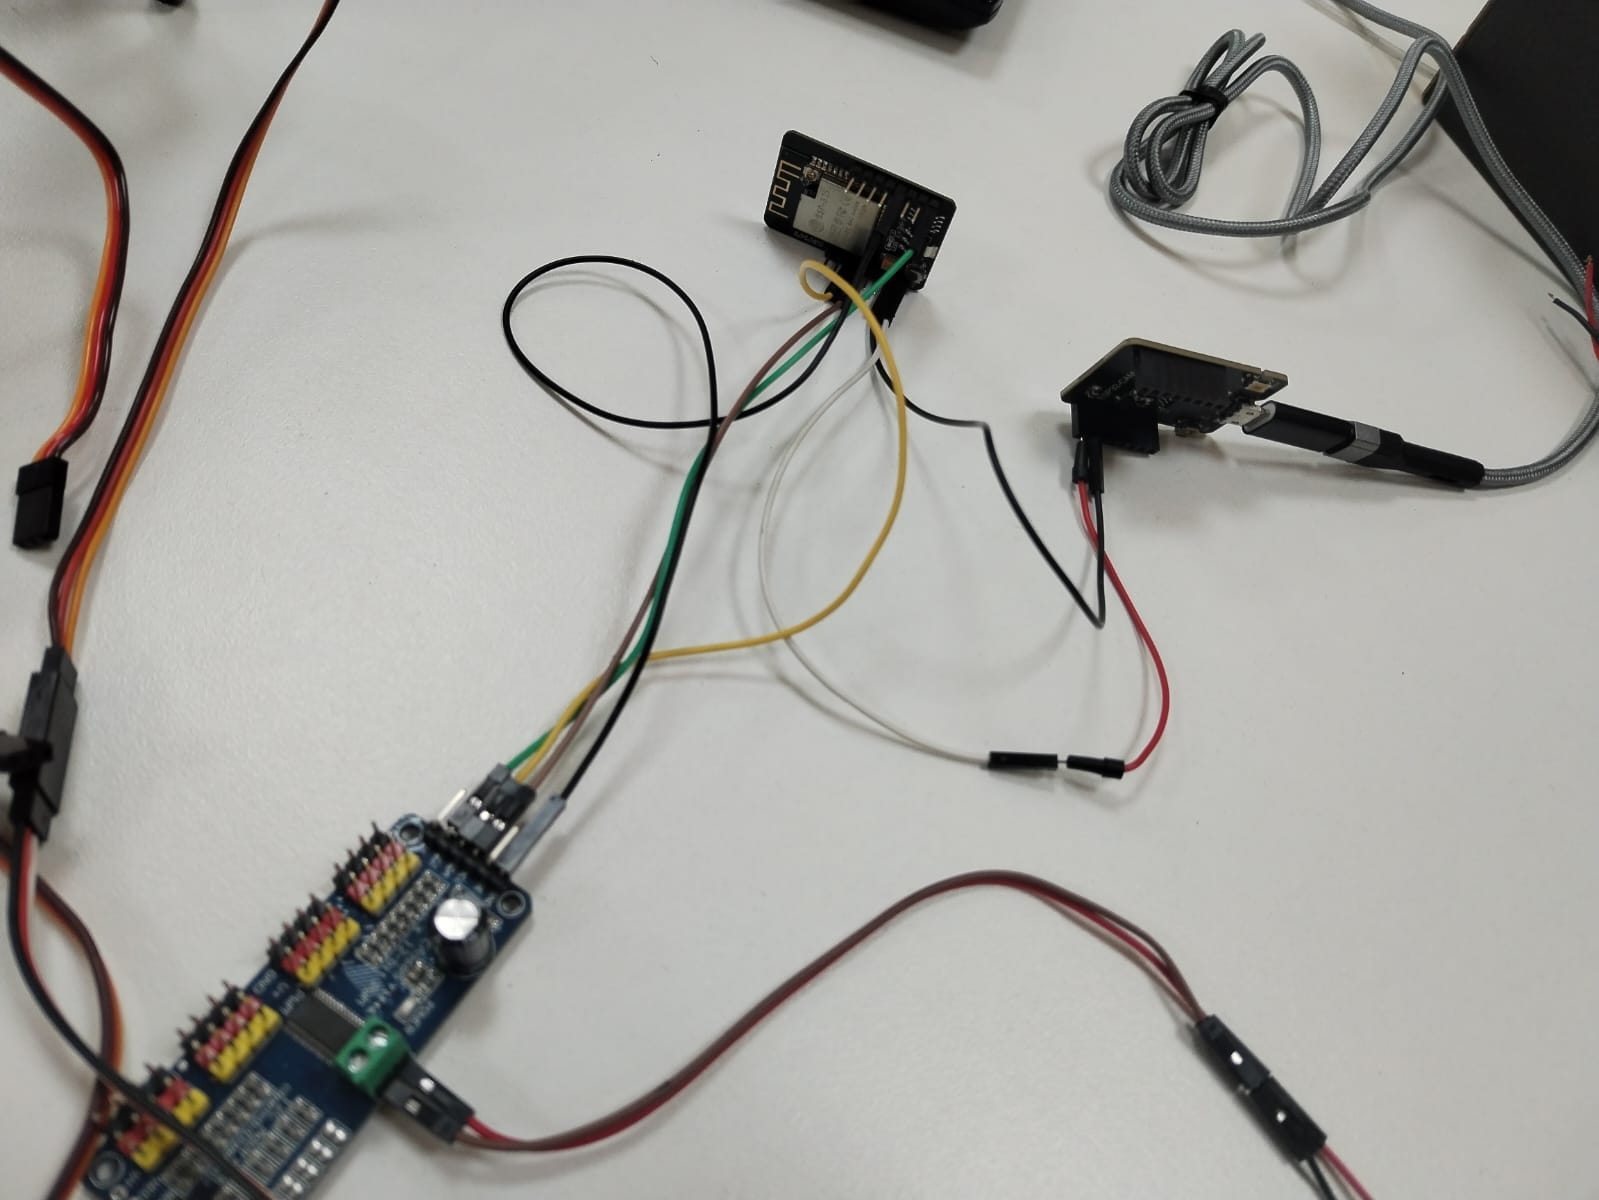
\includegraphics[width=\linewidth,height=7cm,keepaspectratio]{img/evidencia_esp32_pca9685_cableado.jpg}
  \caption{Módulos electrónicos y conductores de interconexión.}
 \end{subfigure}\hfill
 \begin{subfigure}[t]{0.48\textwidth}
  \centering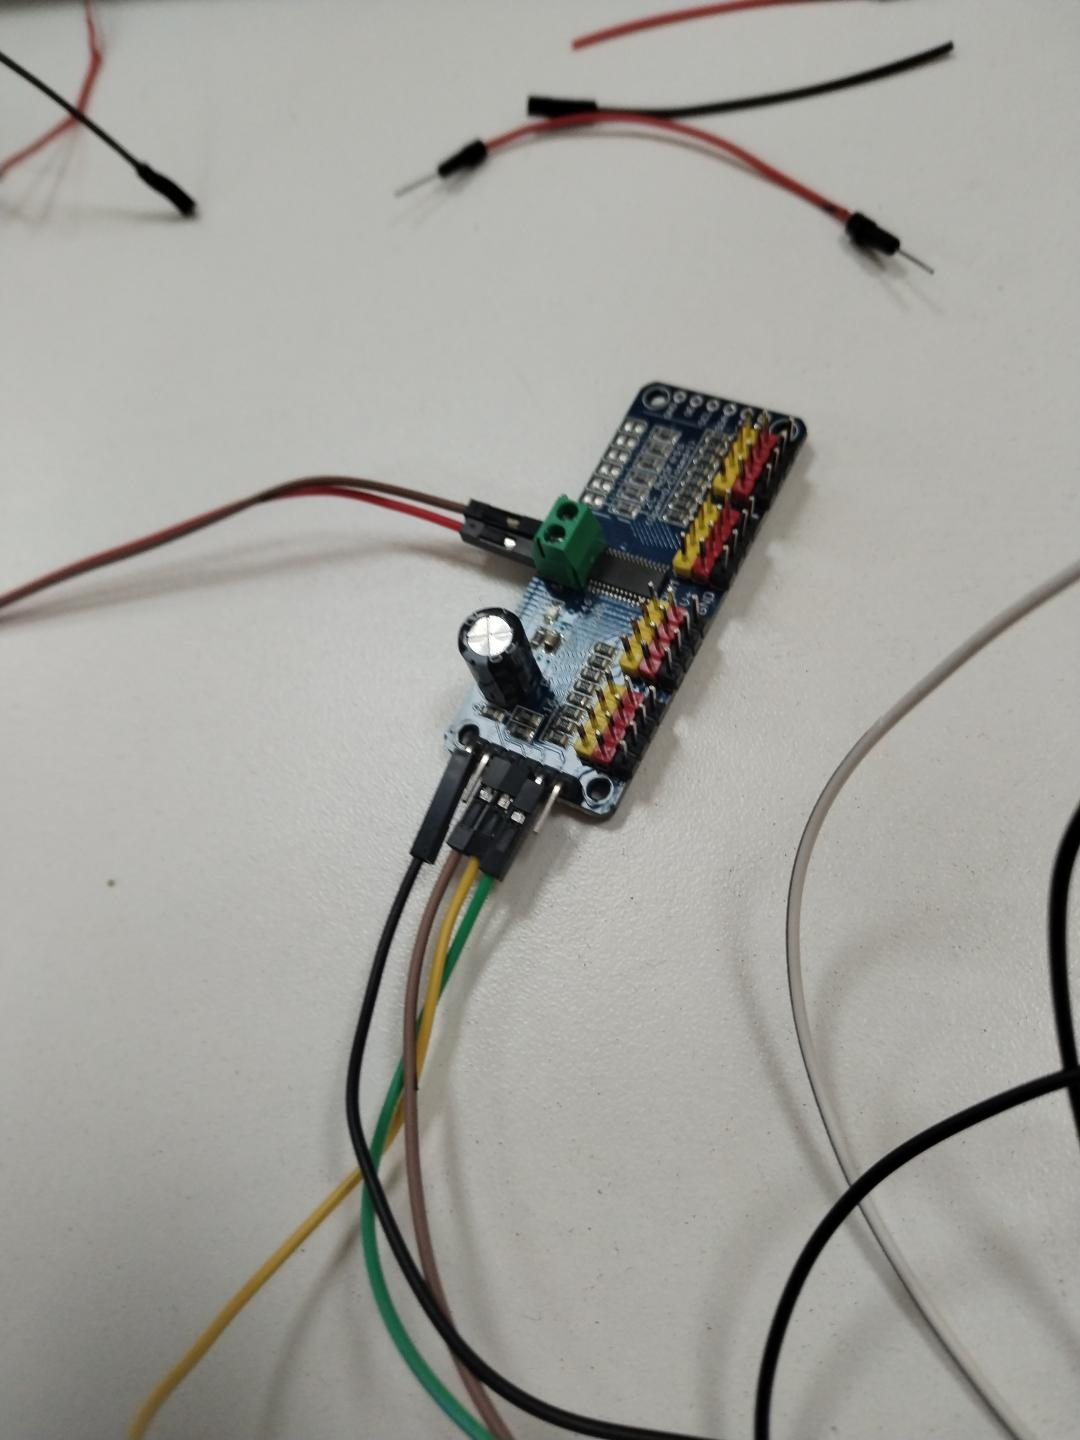
\includegraphics[width=\linewidth,height=7cm,keepaspectratio]{img/evidencia_pca9685_detalle.jpg}
  \caption{Vista cercana del PCA9685 y su bornera.}
 \end{subfigure}
 \caption{Evidencia de avance en la integración del sistema de control electrónico.}
 \label{fig:actualizacion_pca}
\end{figure}

Para validar esta etapa se propone realizar una lectura del bus $I^2C$ con el programa de escaneo del repositorio y registrar el resultado en el monitor serie. Una detección de \texttt{0x40} demostraría comunicación digital con el controlador, pero no permitiría concluir por sí sola que los servomotores estén bien alimentados o que su movimiento sea seguro.

\subsection{Revisión de fuentes de alimentación y baterías}
Las evidencias incluyen un portapilas con dos celdas cilíndricas y una batería plana recargable. Su presencia documenta la evaluación de alternativas de alimentación; no se puede establecer a partir de las fotografías cuál fue conectada durante cada ensayo ni verificar su tensión, capacidad efectiva o corriente disponible. Antes de suministrar energía al riel de servomotores se debe medir la salida con un multímetro y comprobar que la tensión resultante no supere la admisible para el conjunto de servos empleado. No debe asumirse que dos celdas tienen una tensión determinada sin conocer su conexión serie/paralelo y su estado de carga.

\begin{figure}[H]
 \centering
 \begin{subfigure}[t]{0.48\textwidth}
  \centering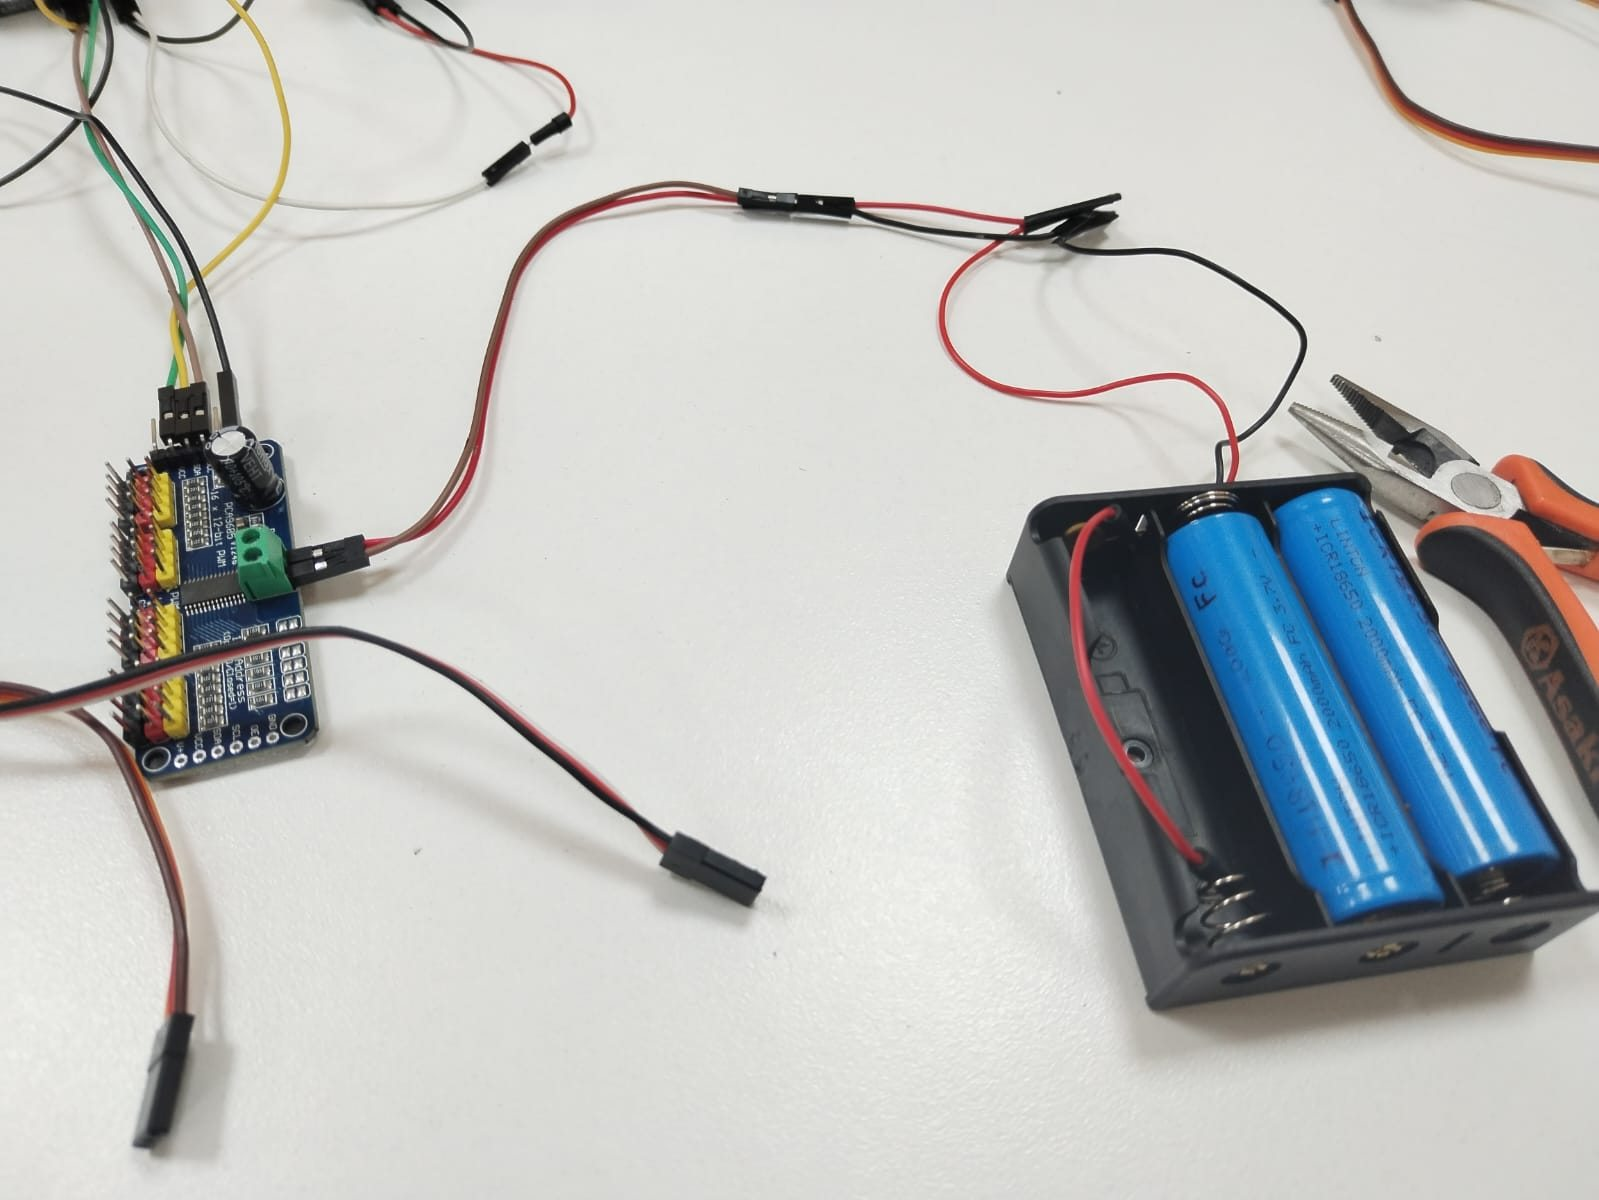
\includegraphics[width=\linewidth,height=7cm,keepaspectratio]{img/evidencia_portapilas_pca9685.jpg}
  \caption{Portapilas de dos celdas junto al PCA9685.}
 \end{subfigure}\hfill
 \begin{subfigure}[t]{0.48\textwidth}
  \centering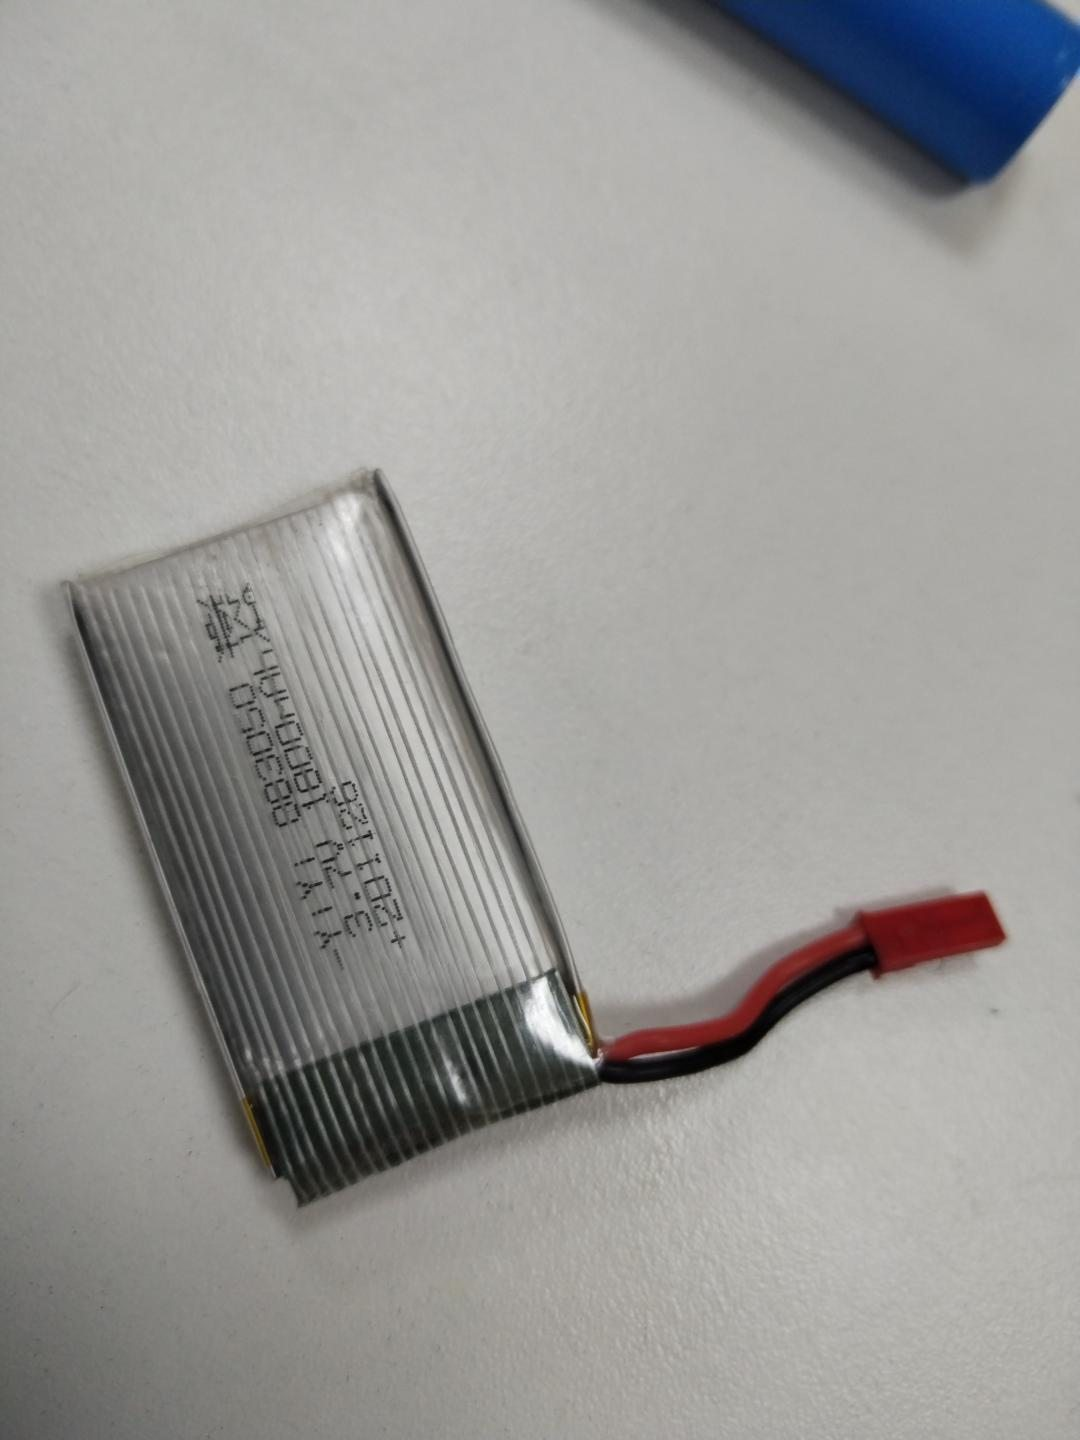
\includegraphics[width=\linewidth,height=7cm,keepaspectratio]{img/evidencia_bateria_lipo.jpg}
  \caption{Batería recargable plana observada en el laboratorio.}
 \end{subfigure}
 \caption{Alternativas de alimentación fotografiadas durante la integración.}
 \label{fig:actualizacion_fuentes}
\end{figure}

Es imprescindible separar la alimentación lógica del ESP32 de la alimentación de potencia de los actuadores, mantener una referencia GND común donde corresponda y utilizar una fuente con corriente suficiente para los picos de los servos. Las baterías de litio requieren protección adecuada contra cortocircuitos, sobrecorriente y descarga excesiva. La desactivación PWM por software no equivale a un interruptor físico de emergencia.

\subsection{Verificación de comunicación local mediante Wi-Fi}
En una captura previa, el teléfono aparece conectado a una red identificada como \texttt{FRANKI-HE}, sin acceso a Internet. Esto es compatible con un funcionamiento en red local: un punto de acceso puede permitir comunicación con dispositivos conectados sin ofrecer salida a Internet. Una segunda captura muestra la dirección privada \texttt{192.168.4.1} con una interfaz web de configuración de la cámara OV2640, incluyendo resolución QVGA (320$\times$240) y controles de exposición, brillo y contraste. Esta captura es evidencia del acceso HTTP a una interfaz de cámara en la red local, aunque no prueba el funcionamiento del panel de servos documentado en el código principal. También debe señalarse que el SSID observado, \texttt{FRANKI-HE}, no coincide con el SSID \texttt{Brazo-ESP32CAM} configurado en la versión revisada de \texttt{brazoR.ino}, por lo que podría corresponder a otra configuración o versión de prueba.

\begin{figure}[H]
 \centering
 \begin{subfigure}[t]{0.48\textwidth}
  \centering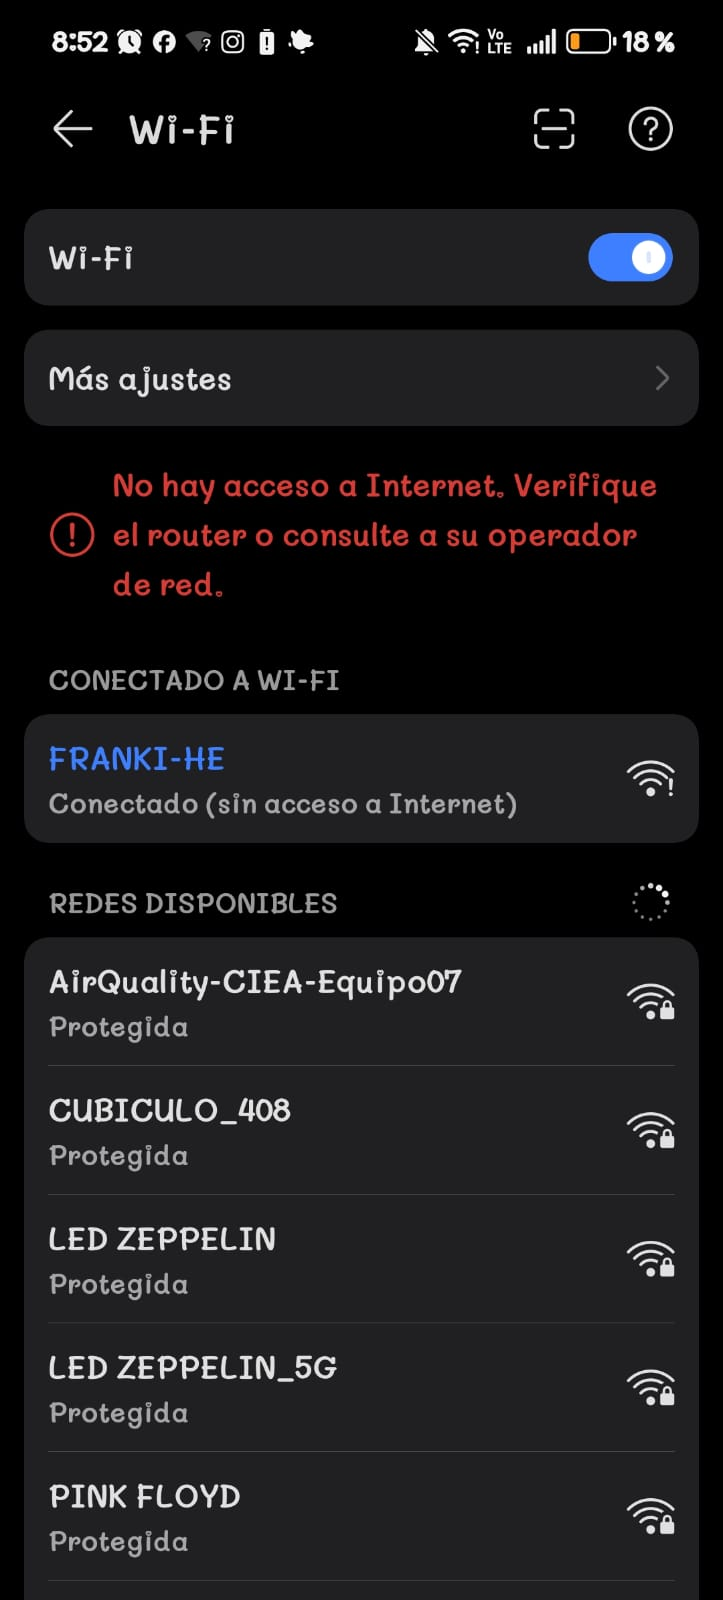
\includegraphics[width=\linewidth,height=9cm,keepaspectratio]{img/evidencia_wifi_red_local.png}
  \caption{Red local \texttt{FRANKI-HE} conectada.}
 \end{subfigure}\hfill
 \begin{subfigure}[t]{0.48\textwidth}
  \centering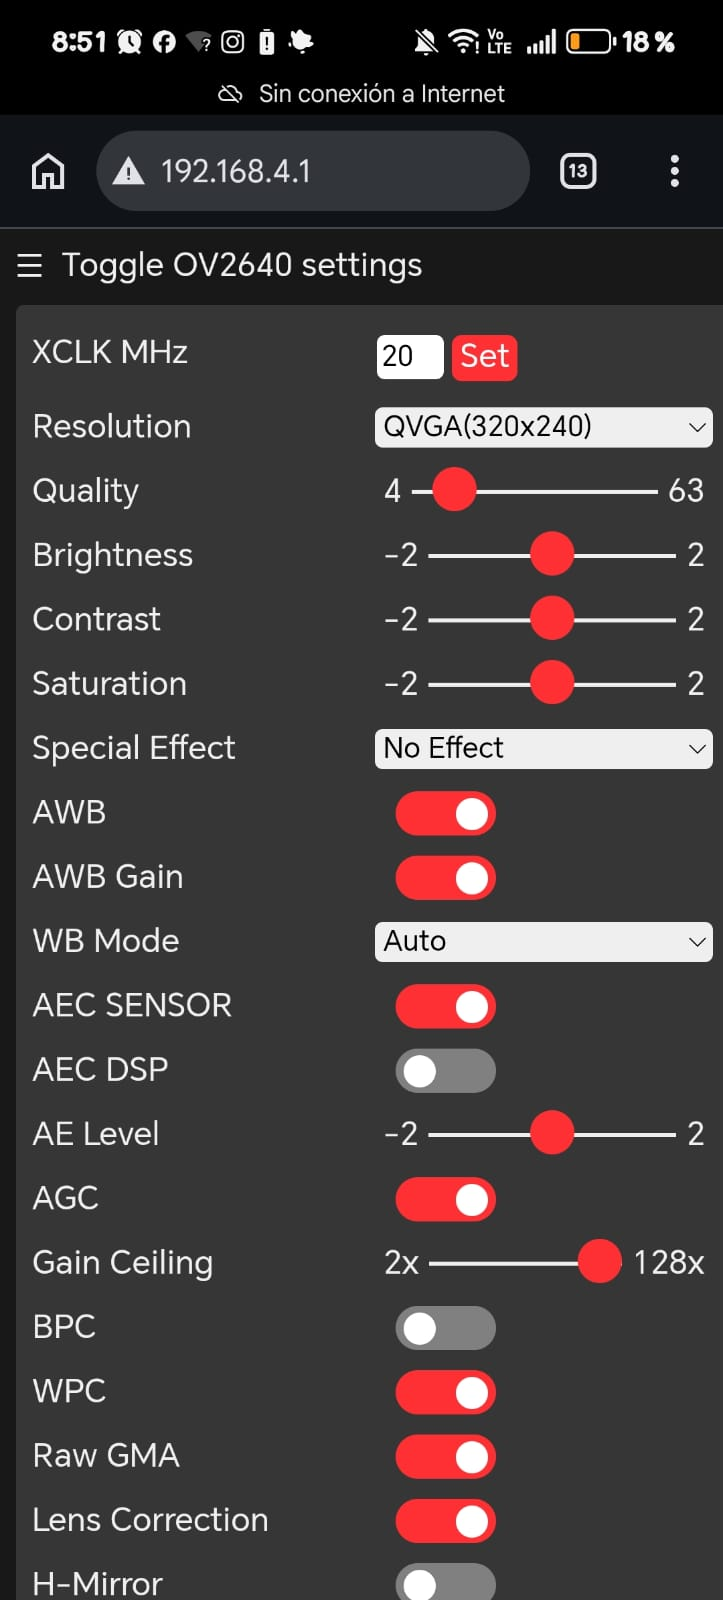
\includegraphics[width=\linewidth,height=9cm,keepaspectratio]{img/evidencia_wifi_panel_ov2640.png}
  \caption{Interfaz OV2640 en \texttt{192.168.4.1}.}
 \end{subfigure}
 \caption{Evidencias de comunicación inalámbrica y acceso web desde un dispositivo móvil.}
 \label{fig:actualizacion_wifi}
\end{figure}

\subsection{Procedimiento de calibración y comprobaciones pendientes}
Para pasar del ensamblaje observado a una calibración verificable se propone: (i) desenergizar y asegurar mecánicamente las uniones; (ii) confirmar el apriete de los servocuernos y la ausencia de holguras; (iii) alimentar un solo servo con una fuente medida y adecuada; (iv) comprobar el centro nominal de $90^\circ$ antes de fijar el eslabón; (v) recorrer gradualmente los límites evitando topes; y (vi) repetir el procedimiento articulación por articulación. El programa del repositorio utiliza límites nominales de $30^\circ$ a $150^\circ$ y debe ajustarse según el espacio mecánico real.

\begin{table}[H]
\centering\small
\caption{Registro de verificaciones y estado de evidencia disponible}
\label{tab:actualizacion_verificaciones}
\begin{tabularx}{\textwidth}{p{4.0cm} X p{3.2cm}}
\toprule
\textbf{Elemento} & \textbf{Evidencia o criterio} & \textbf{Estado documentado}\\
\midrule
Montaje de eslabones & Fotografías del brazo en varias posturas. & Observado\\
Controlador PCA9685 & Fotografías del módulo y del cableado. & Montaje observado\\
Comunicación Wi-Fi & Capturas de red local e interfaz OV2640. & Acceso web observado\\
Tensión de alimentación & Lectura con multímetro y polaridad. & Sin medida aportada\\
Ángulos reales & Comparación entre orden y medición física. & Sin medida aportada\\
Movimiento de seis servos & Ensayo individual con registro de resultados. & No demostrado por las fotos\\
\bottomrule
\end{tabularx}
\end{table}

\subsection{Balance del avance experimental}
Respecto a la documentación previa, las fotografías aportan evidencia adicional de integración física del brazo, presencia de cableado electrónico, disposición del PCA9685, inspección de alimentaciones y acceso a una interfaz web local. Sin embargo, sería incorrecto transformar estas observaciones en resultados cuantitativos de exactitud o autonomía sin mediciones. Como siguiente etapa se recomienda anexar una tabla con tensión de alimentación en reposo y bajo carga, lectura de corriente, posición angular ordenada y observada para cada articulación, y resultado de las pruebas de comunicación y movimiento.

% Usa paquetes ya presentes en main.tex: graphicx, float, booktabs, tabularx, subcaption.

\section{Actualización experimental: ensamble, conexiones y ajustes del manipulador}
\label{sec:actualizacion_evidencias}

\subsection{Objeto y alcance del registro fotográfico}
Las evidencias recopiladas corresponden a una nueva etapa de integración del brazo robótico articulado. Se observan diferentes configuraciones mecánicas del manipulador, el montaje de un controlador PWM PCA9685, un módulo de la familia ESP32, conexiones mediante cables y elementos empleados para evaluar la alimentación eléctrica. El propósito de esta sección es registrar el progreso físico del prototipo y delimitar las comprobaciones que aún se requieren. Las fotografías son evidencia de montaje, pero no constituyen por sí mismas una medida de precisión, par disponible o estabilidad eléctrica.

\subsection{Progreso del ensamblaje y postura de las articulaciones}
El manipulador conserva una estructura de eslabones rígidos, servomotores montados en soportes metálicos, pinza mecánica y base de madera. Las nuevas imágenes muestran posiciones inclinadas, frontales y casi verticales, útiles para observar la alineación relativa de hombro, codo y muñeca. Estas posiciones sirven como referencia para identificar posibles interferencias, puntos de holgura y distribución del cableado. No se dispone de un registro instrumental de los ángulos reales, por lo que la denominación ``calibración'' se emplea aquí para describir el proceso de ajuste y verificación, no para afirmar que haya concluido.

\begin{figure}[H]
 \centering
 \begin{subfigure}[t]{0.48\textwidth}
  \centering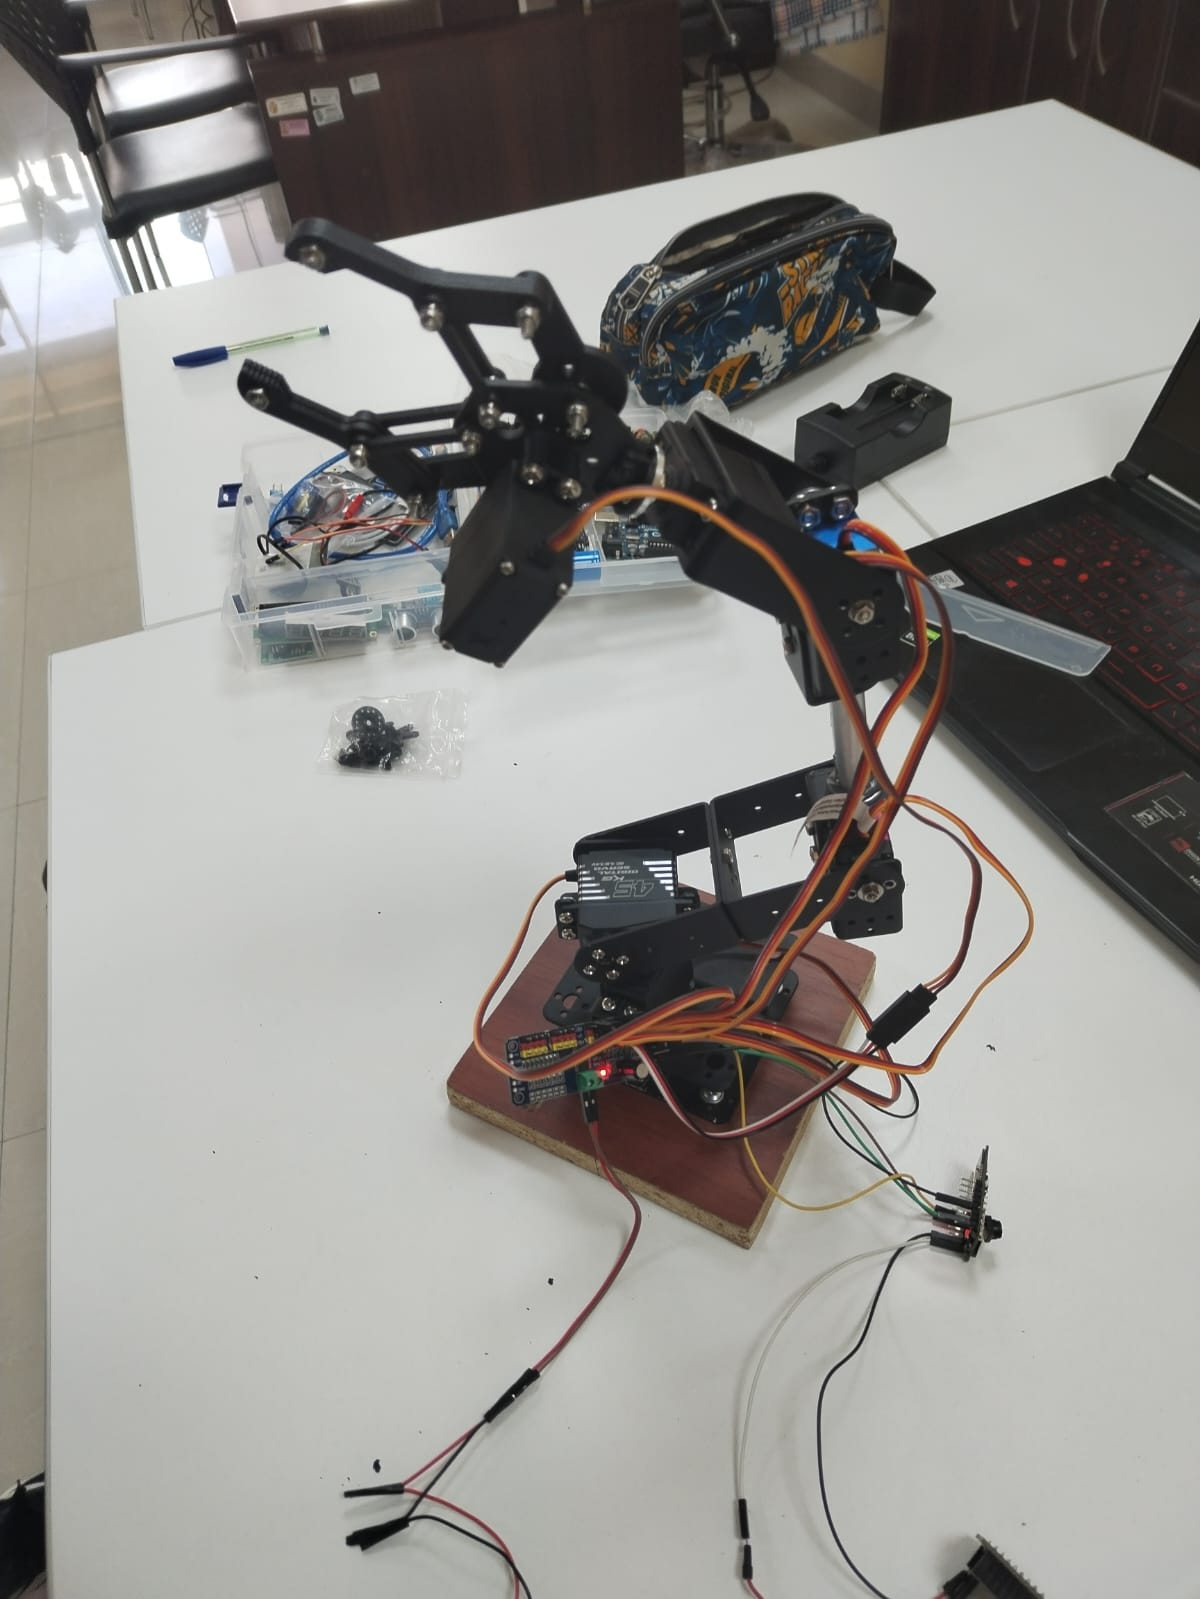
\includegraphics[width=\linewidth,height=7cm,keepaspectratio]{img/evidencia_brazo_integracion_lateral.jpg}
  \caption{Vista lateral durante la integración de la pinza y los eslabones.}
 \end{subfigure}\hfill
 \begin{subfigure}[t]{0.48\textwidth}
  \centering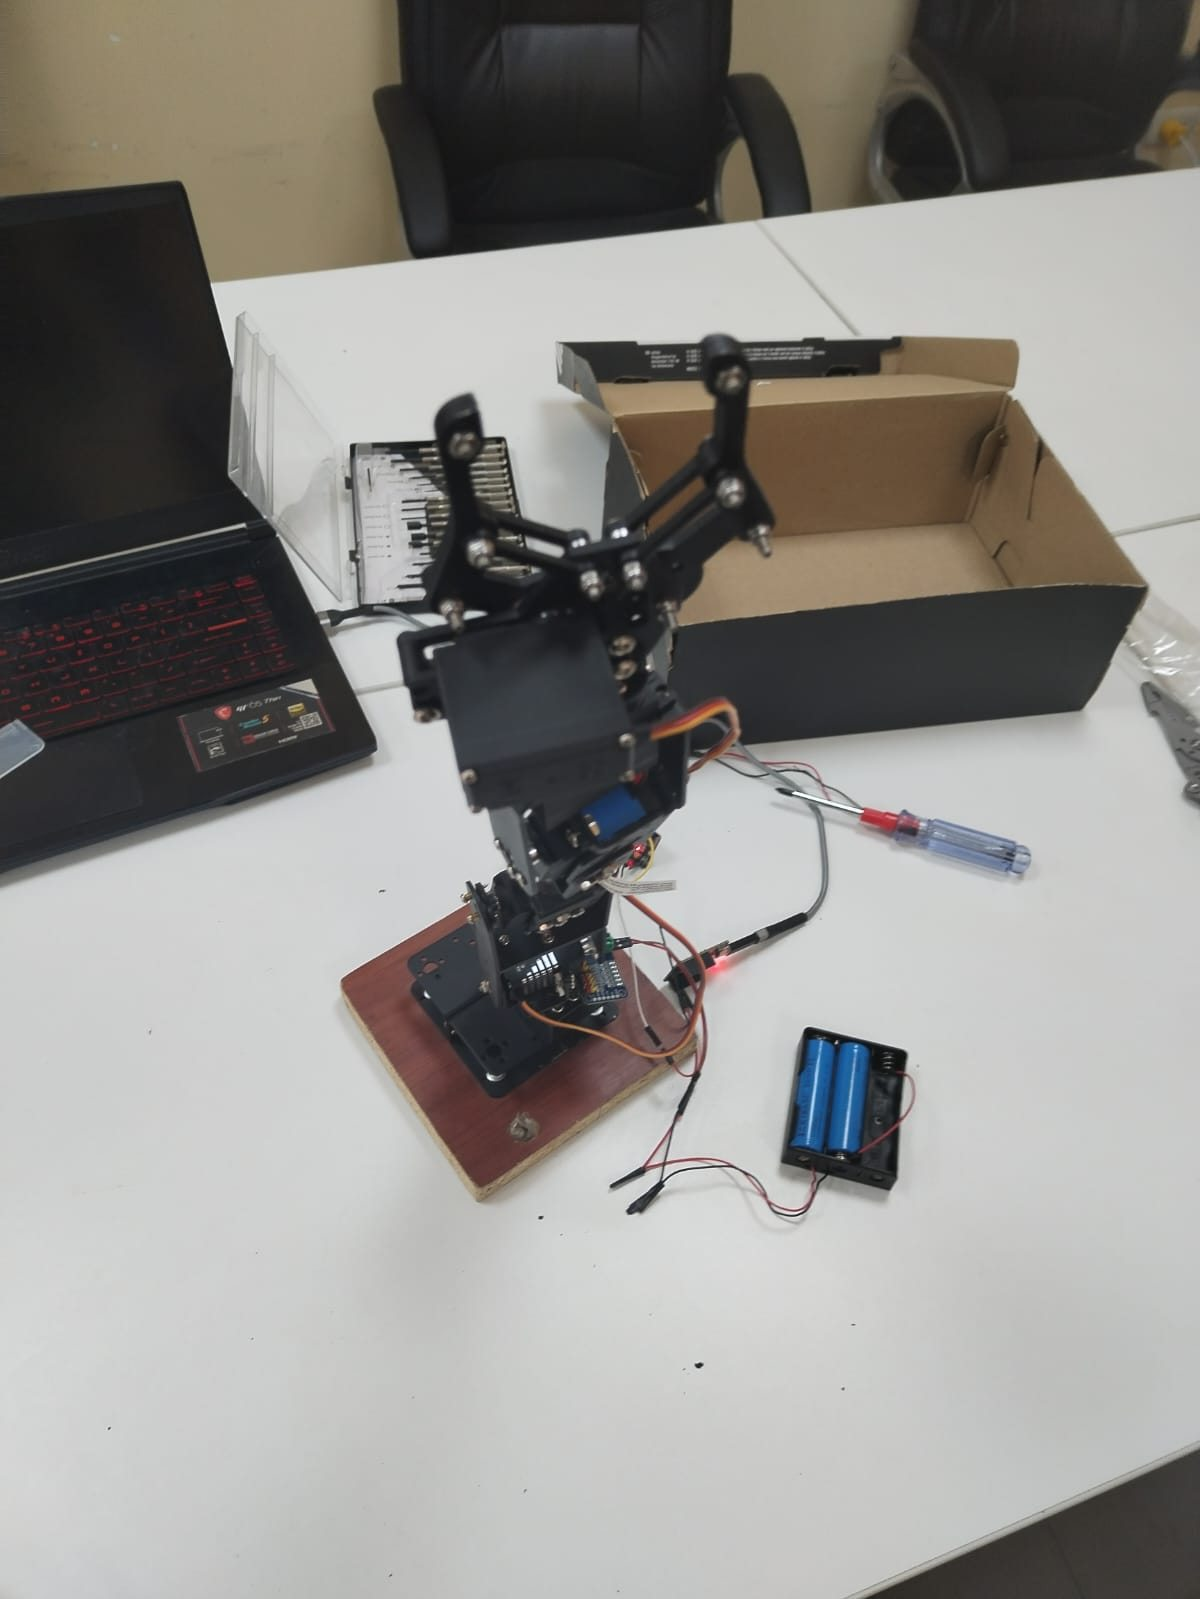
\includegraphics[width=\linewidth,height=7cm,keepaspectratio]{img/evidencia_brazo_vista_frontal.jpg}
  \caption{Vista frontal del conjunto articulado en banco de trabajo.}
 \end{subfigure}
 \caption{Registro del ensamble físico en diferentes orientaciones.}
 \label{fig:actualizacion_ensamble}
\end{figure}

\begin{figure}[H]
 \centering
 \begin{subfigure}[t]{0.48\textwidth}
  \centering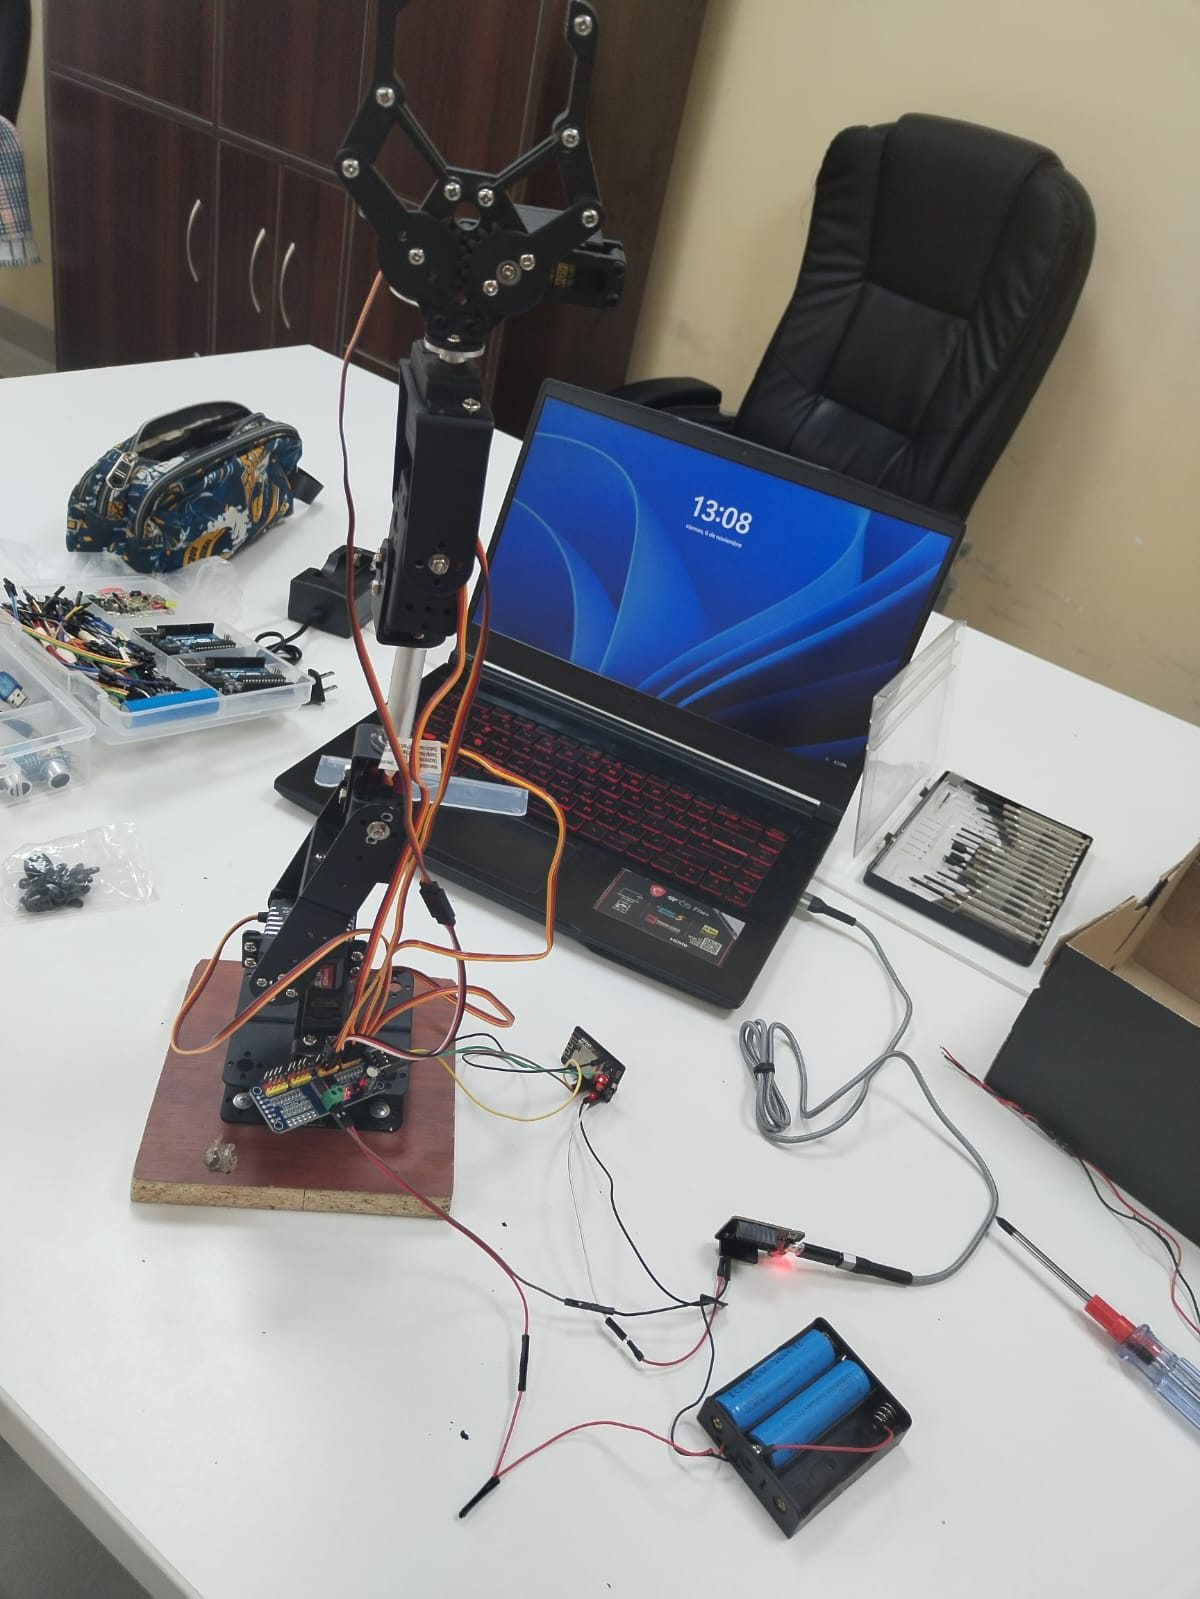
\includegraphics[width=\linewidth,height=7cm,keepaspectratio]{img/evidencia_brazo_postura_vertical.jpg}
  \caption{Prototipo con el efector final elevado.}
 \end{subfigure}\hfill
 \begin{subfigure}[t]{0.48\textwidth}
  \centering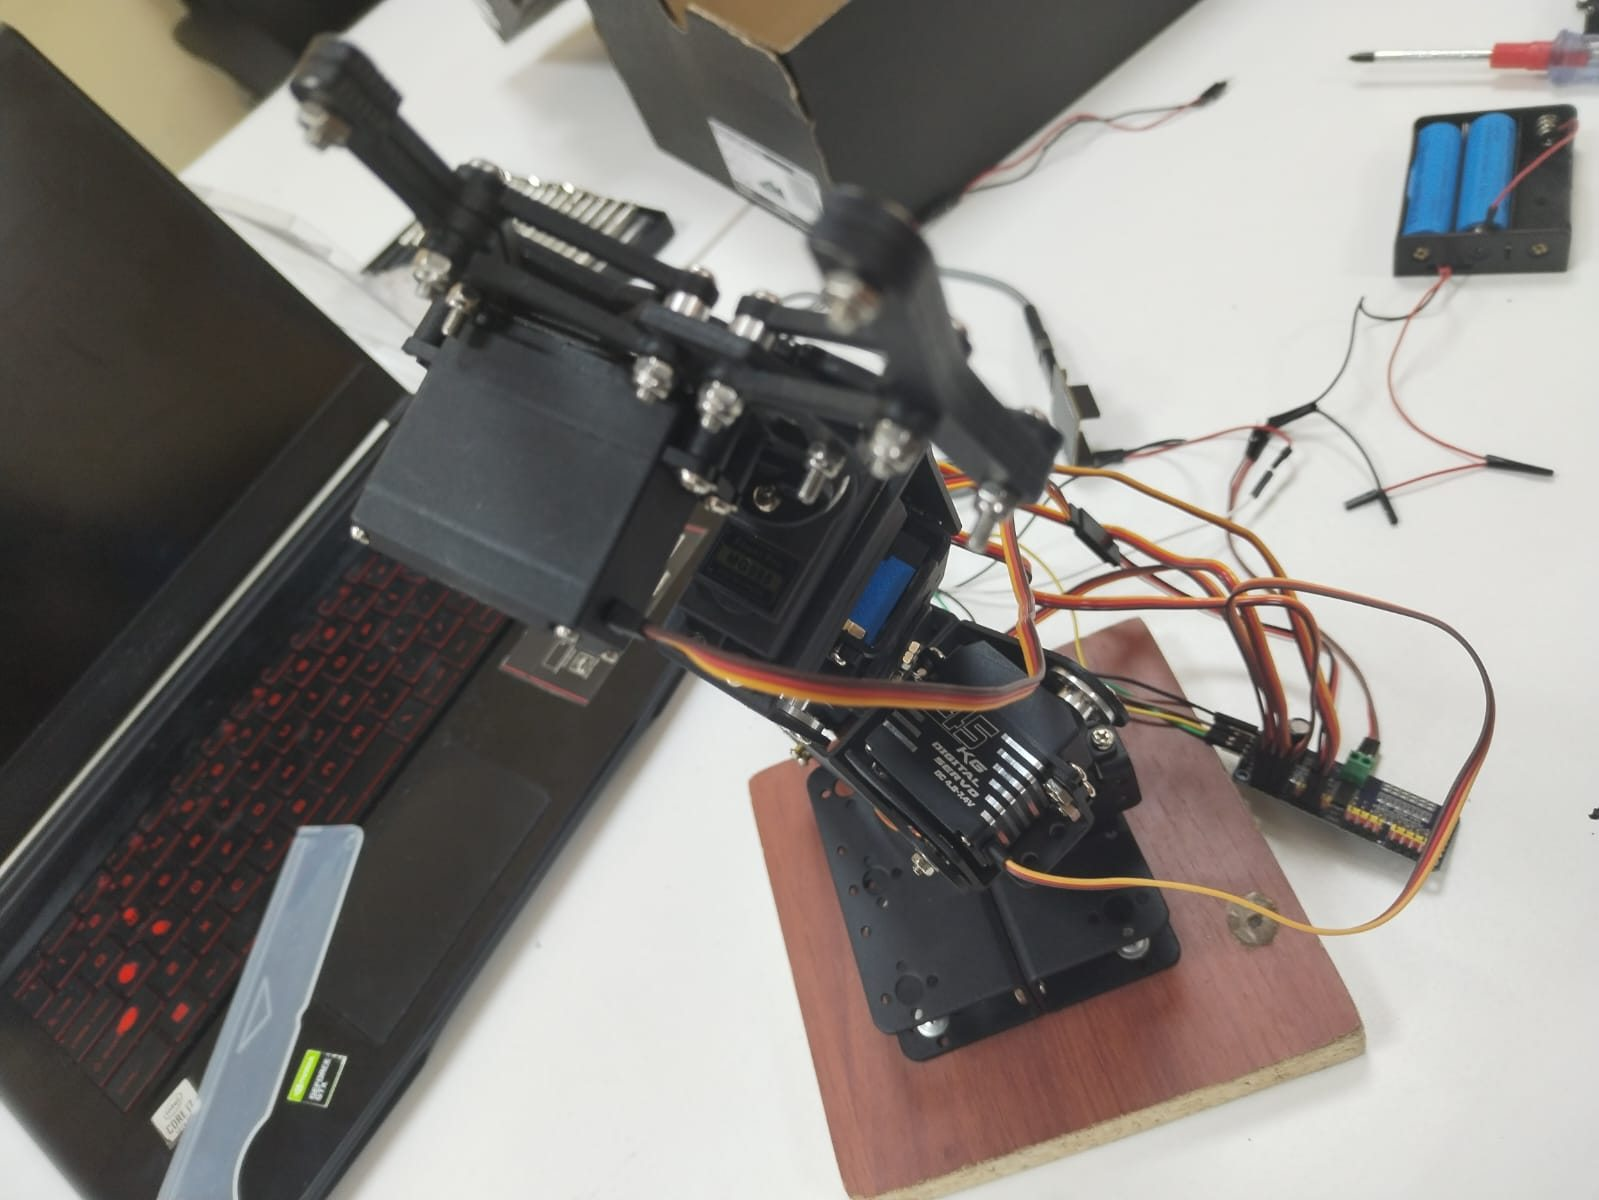
\includegraphics[width=\linewidth,height=7cm,keepaspectratio]{img/evidencia_brazo_articulaciones_closeup.jpg}
  \caption{Detalle de los soportes y uniones cercanos a la pinza.}
 \end{subfigure}
 \caption{Posturas de referencia para la revisión de alineación y holguras.}
 \label{fig:actualizacion_posturas}
\end{figure}

\begin{figure}[H]
 \centering
 \begin{subfigure}[t]{0.48\textwidth}
  \centering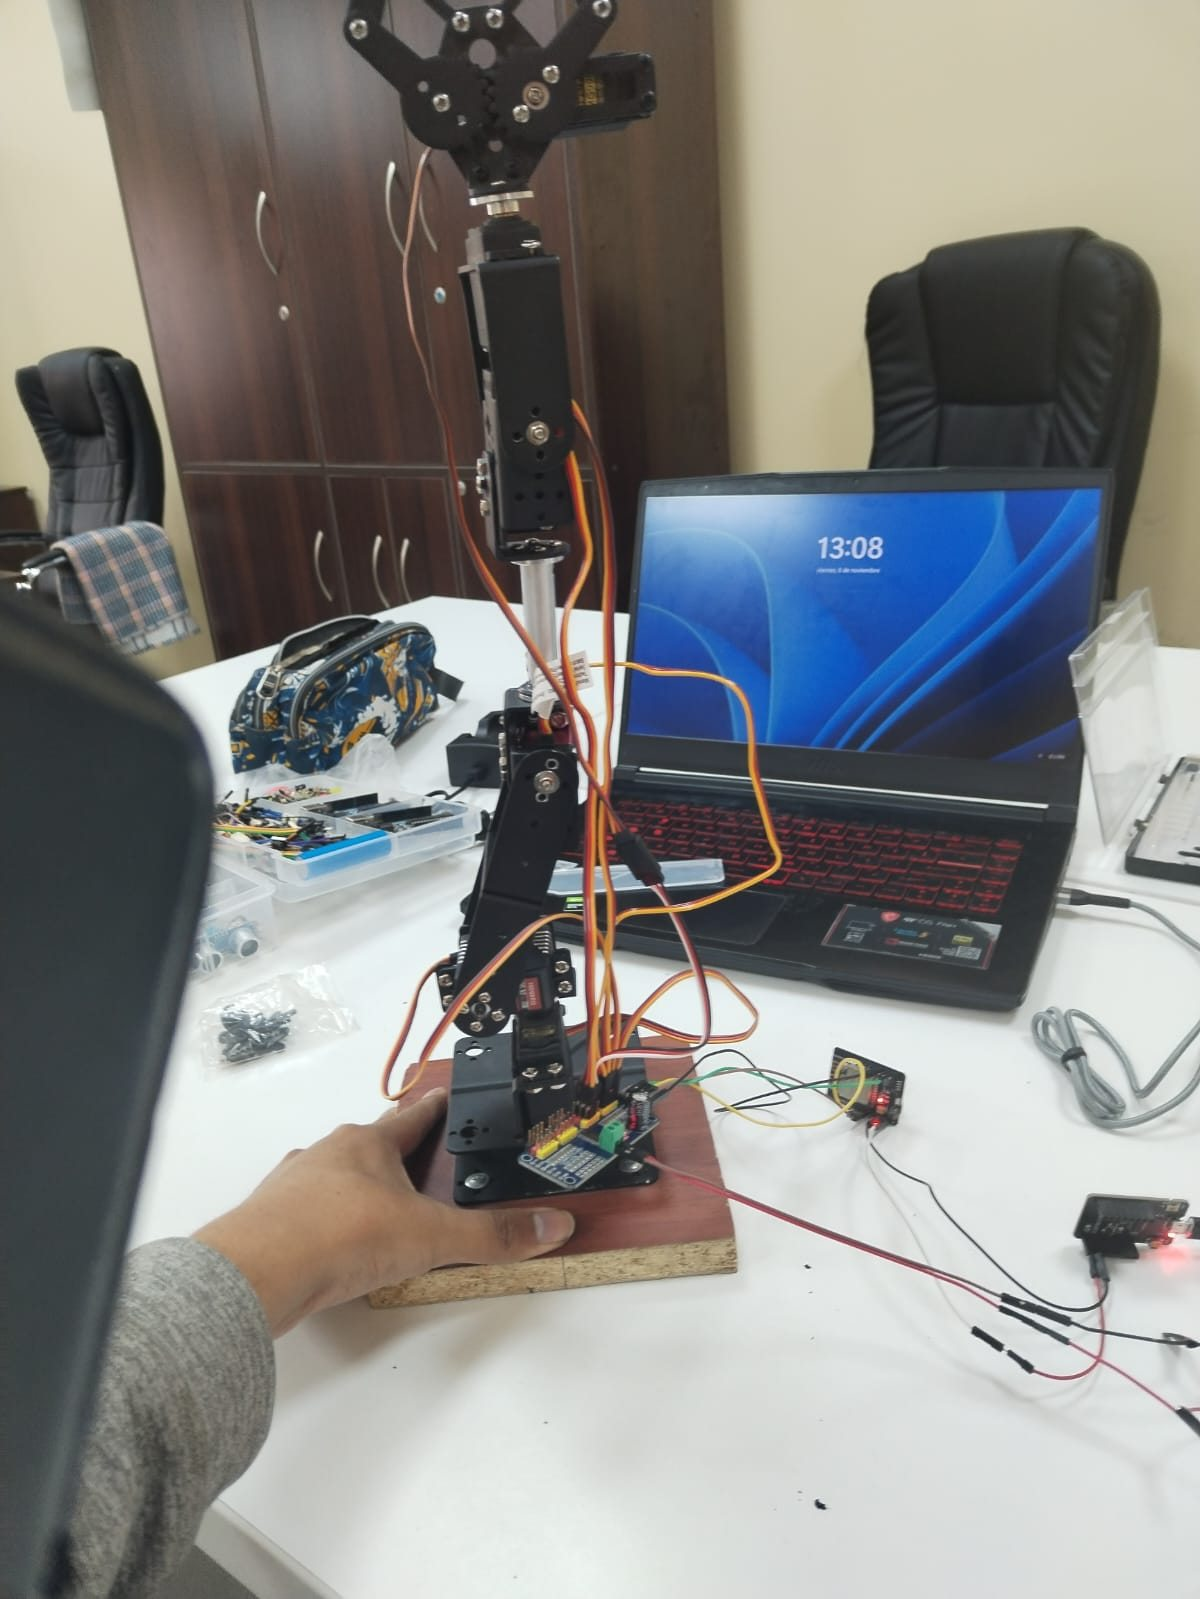
\includegraphics[width=\linewidth,height=7cm,keepaspectratio]{img/evidencia_brazo_estabilidad_base.jpg}
  \caption{Sujeción manual del conjunto a su base.}
 \end{subfigure}\hfill
 \begin{subfigure}[t]{0.48\textwidth}
  \centering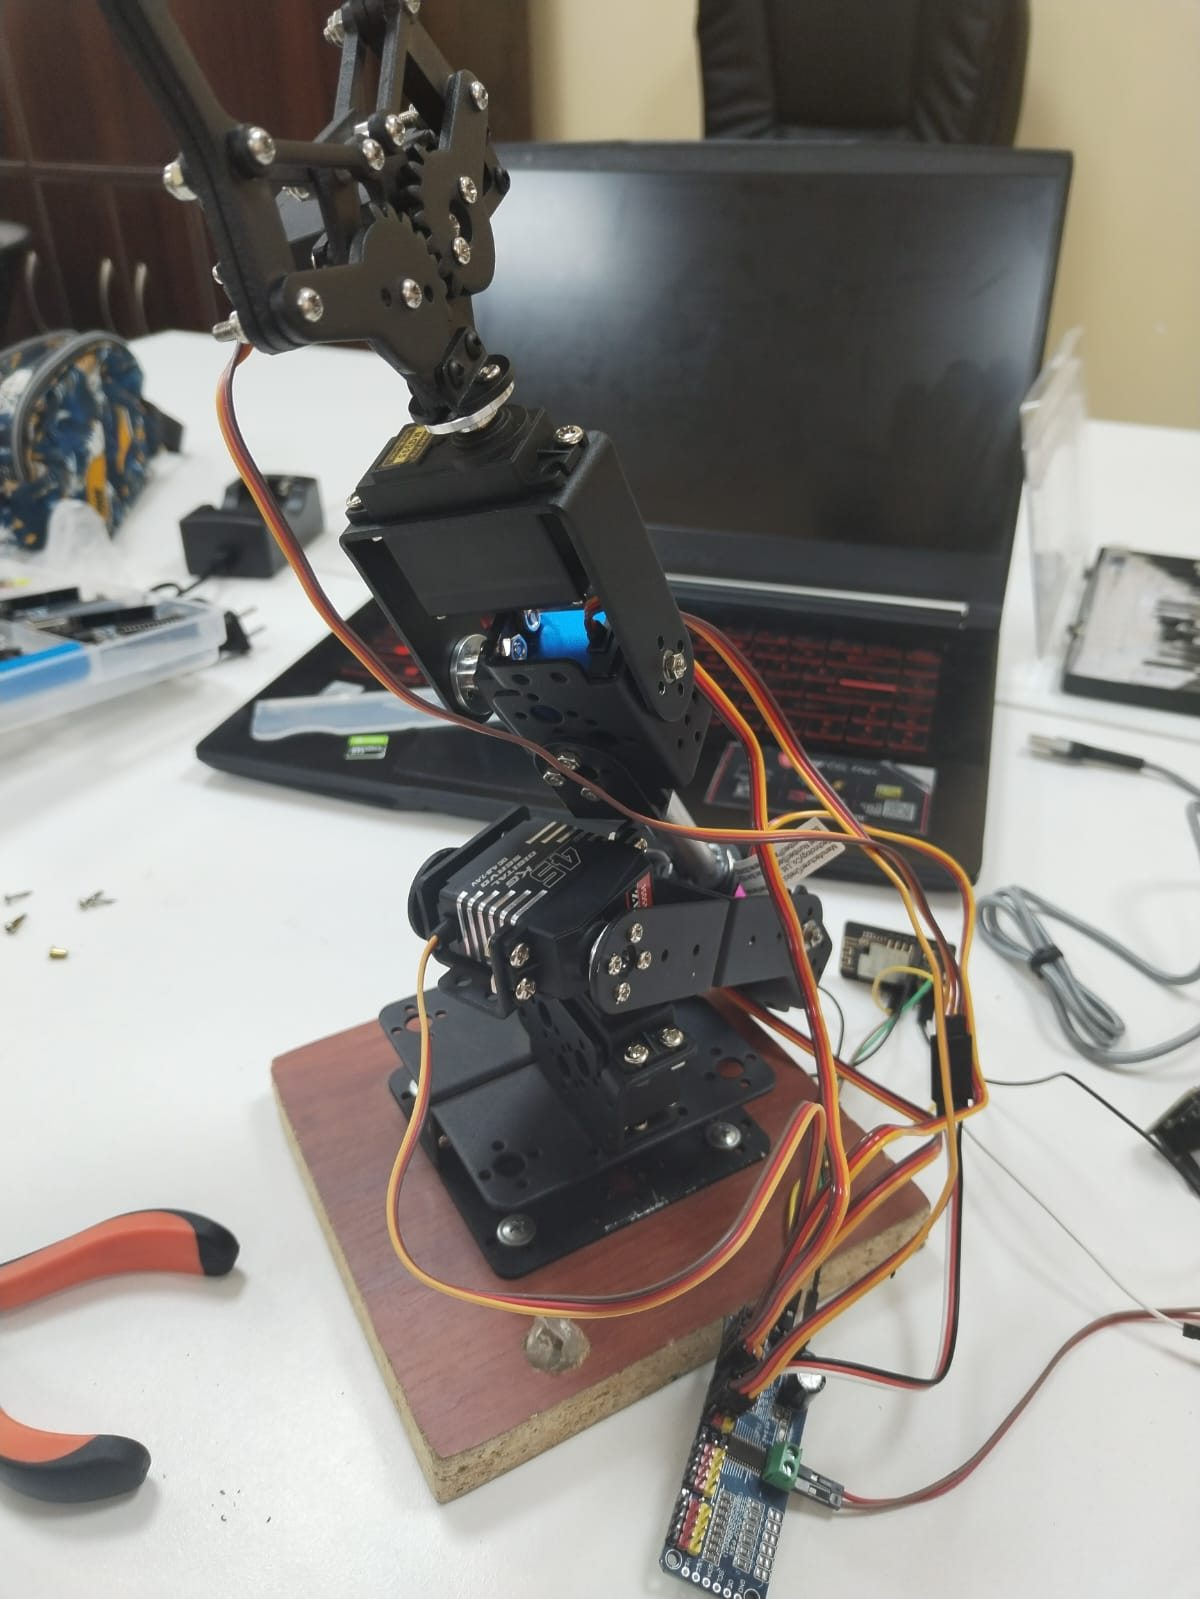
\includegraphics[width=\linewidth,height=7cm,keepaspectratio]{img/evidencia_brazo_soportes_mecanicos.jpg}
  \caption{Vista cercana de servomotores, soportes y tornillería.}
 \end{subfigure}
 \caption{Inspección mecánica de las articulaciones y la plataforma soporte.}
 \label{fig:actualizacion_base}
\end{figure}

\subsection{Integración del ESP32 y del controlador PCA9685}
En las imágenes se reconoce el módulo PCA9685, cuyas cabeceras distribuyen las señales de control hacia los servomotores. El controlador recibe las órdenes por el bus $I^2C$ y genera las señales PWM independientemente del procesador. La fotografía del cableado permite observar conexiones entre módulos, aunque no basta para certificar continuidad, polaridad o asignación exacta de cada conductor. En el firmware del repositorio se configuran de forma nominal SDA en GPIO 13, SCL en GPIO 14 y dirección $I^2C$ \texttt{0x40}; estos valores deben contrastarse con el montaje realmente utilizado.

\begin{figure}[H]
 \centering
 \begin{subfigure}[t]{0.48\textwidth}
  \centering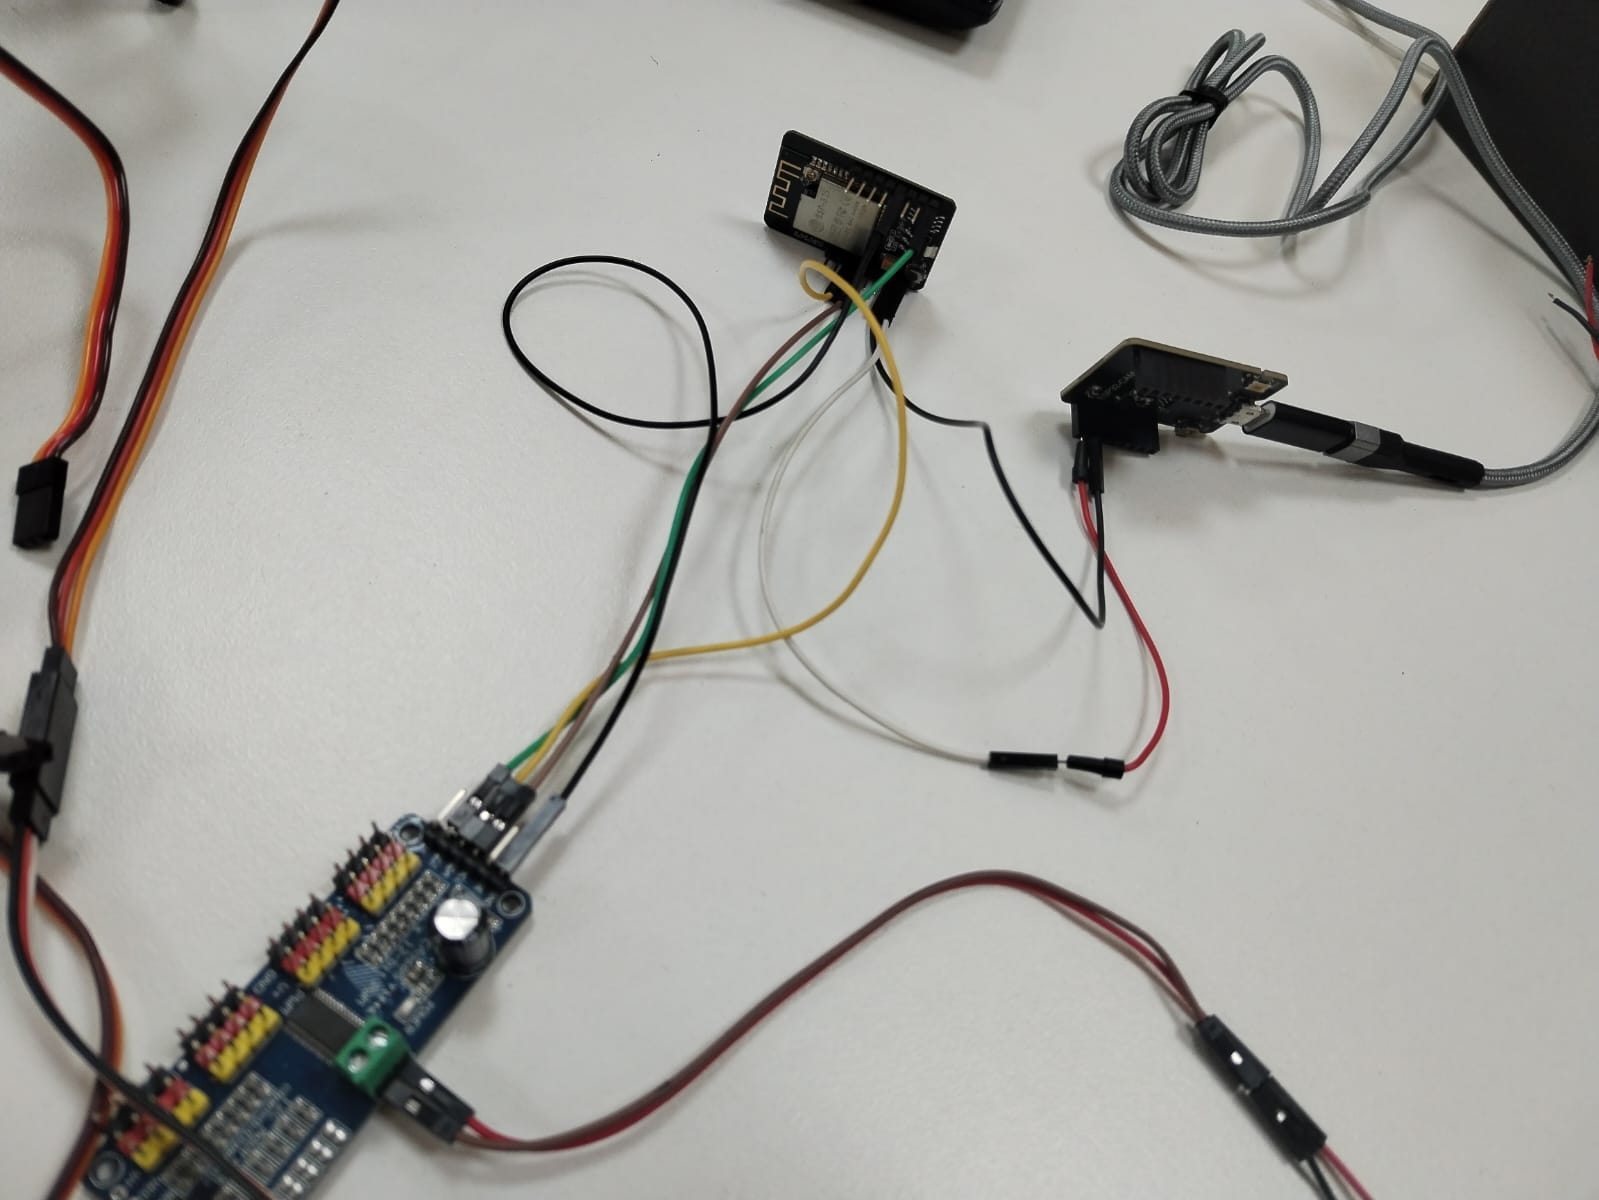
\includegraphics[width=\linewidth,height=7cm,keepaspectratio]{img/evidencia_esp32_pca9685_cableado.jpg}
  \caption{Módulos electrónicos y conductores de interconexión.}
 \end{subfigure}\hfill
 \begin{subfigure}[t]{0.48\textwidth}
  \centering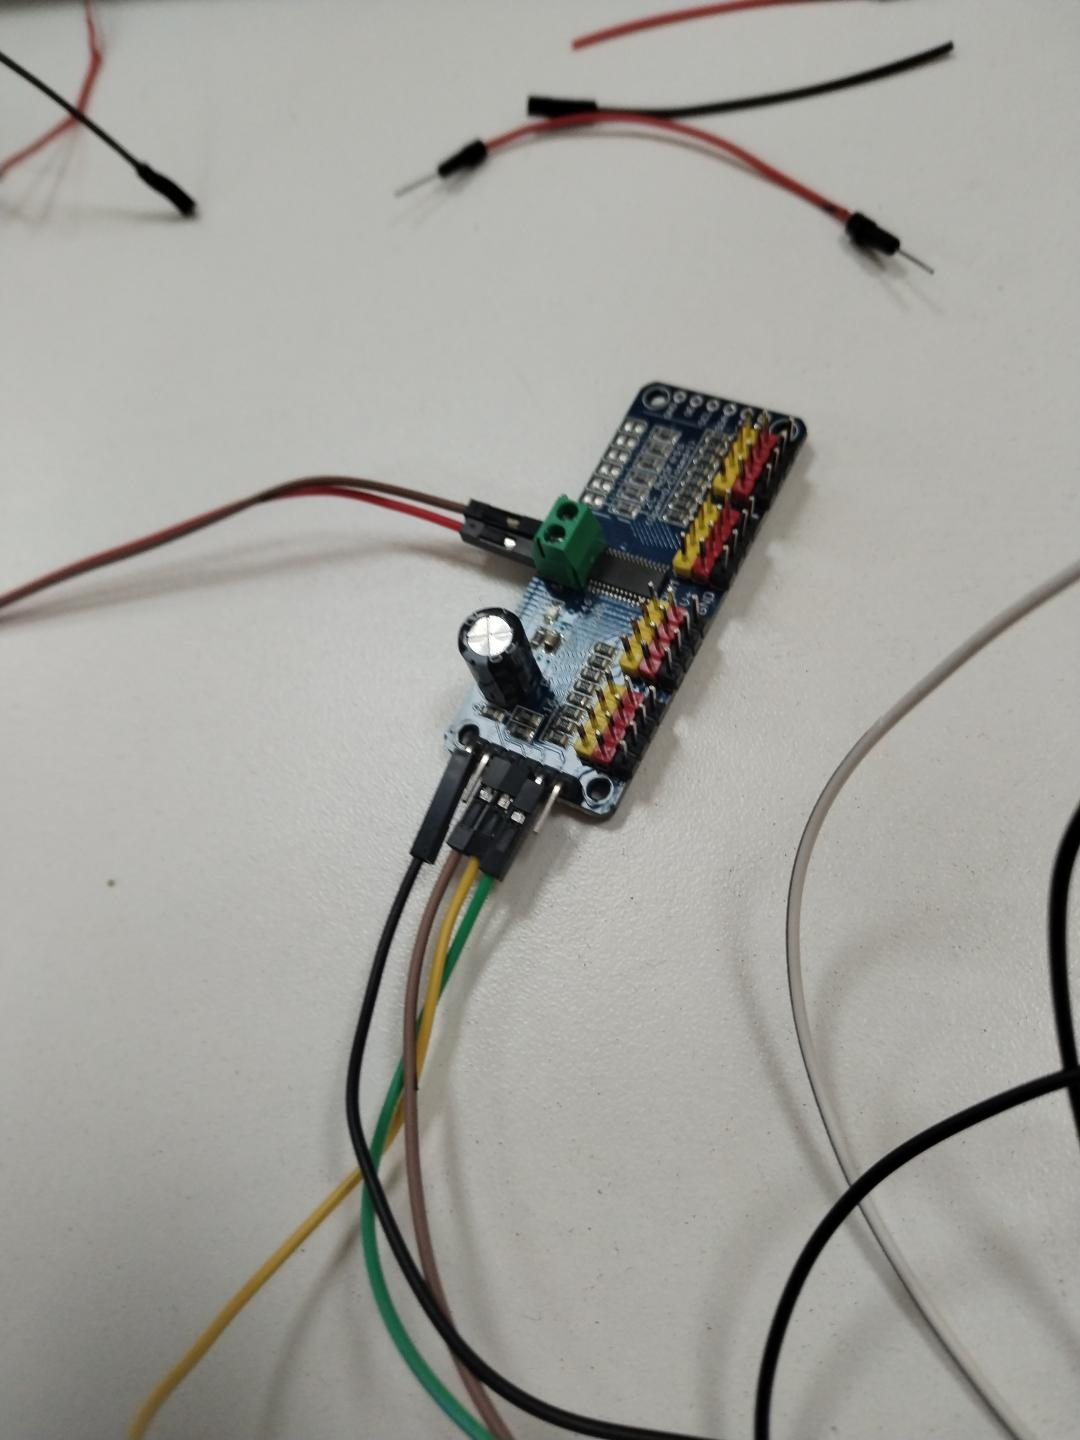
\includegraphics[width=\linewidth,height=7cm,keepaspectratio]{img/evidencia_pca9685_detalle.jpg}
  \caption{Vista cercana del PCA9685 y su bornera.}
 \end{subfigure}
 \caption{Evidencia de avance en la integración del sistema de control electrónico.}
 \label{fig:actualizacion_pca}
\end{figure}

Para validar esta etapa se propone realizar una lectura del bus $I^2C$ con el programa de escaneo del repositorio y registrar el resultado en el monitor serie. Una detección de \texttt{0x40} demostraría comunicación digital con el controlador, pero no permitiría concluir por sí sola que los servomotores estén bien alimentados o que su movimiento sea seguro.

\subsection{Revisión de fuentes de alimentación y baterías}
Las evidencias incluyen un portapilas con dos celdas cilíndricas y una batería plana recargable. Su presencia documenta la evaluación de alternativas de alimentación; no se puede establecer a partir de las fotografías cuál fue conectada durante cada ensayo ni verificar su tensión, capacidad efectiva o corriente disponible. Antes de suministrar energía al riel de servomotores se debe medir la salida con un multímetro y comprobar que la tensión resultante no supere la admisible para el conjunto de servos empleado. No debe asumirse que dos celdas tienen una tensión determinada sin conocer su conexión serie/paralelo y su estado de carga.

\begin{figure}[H]
 \centering
 \begin{subfigure}[t]{0.48\textwidth}
  \centering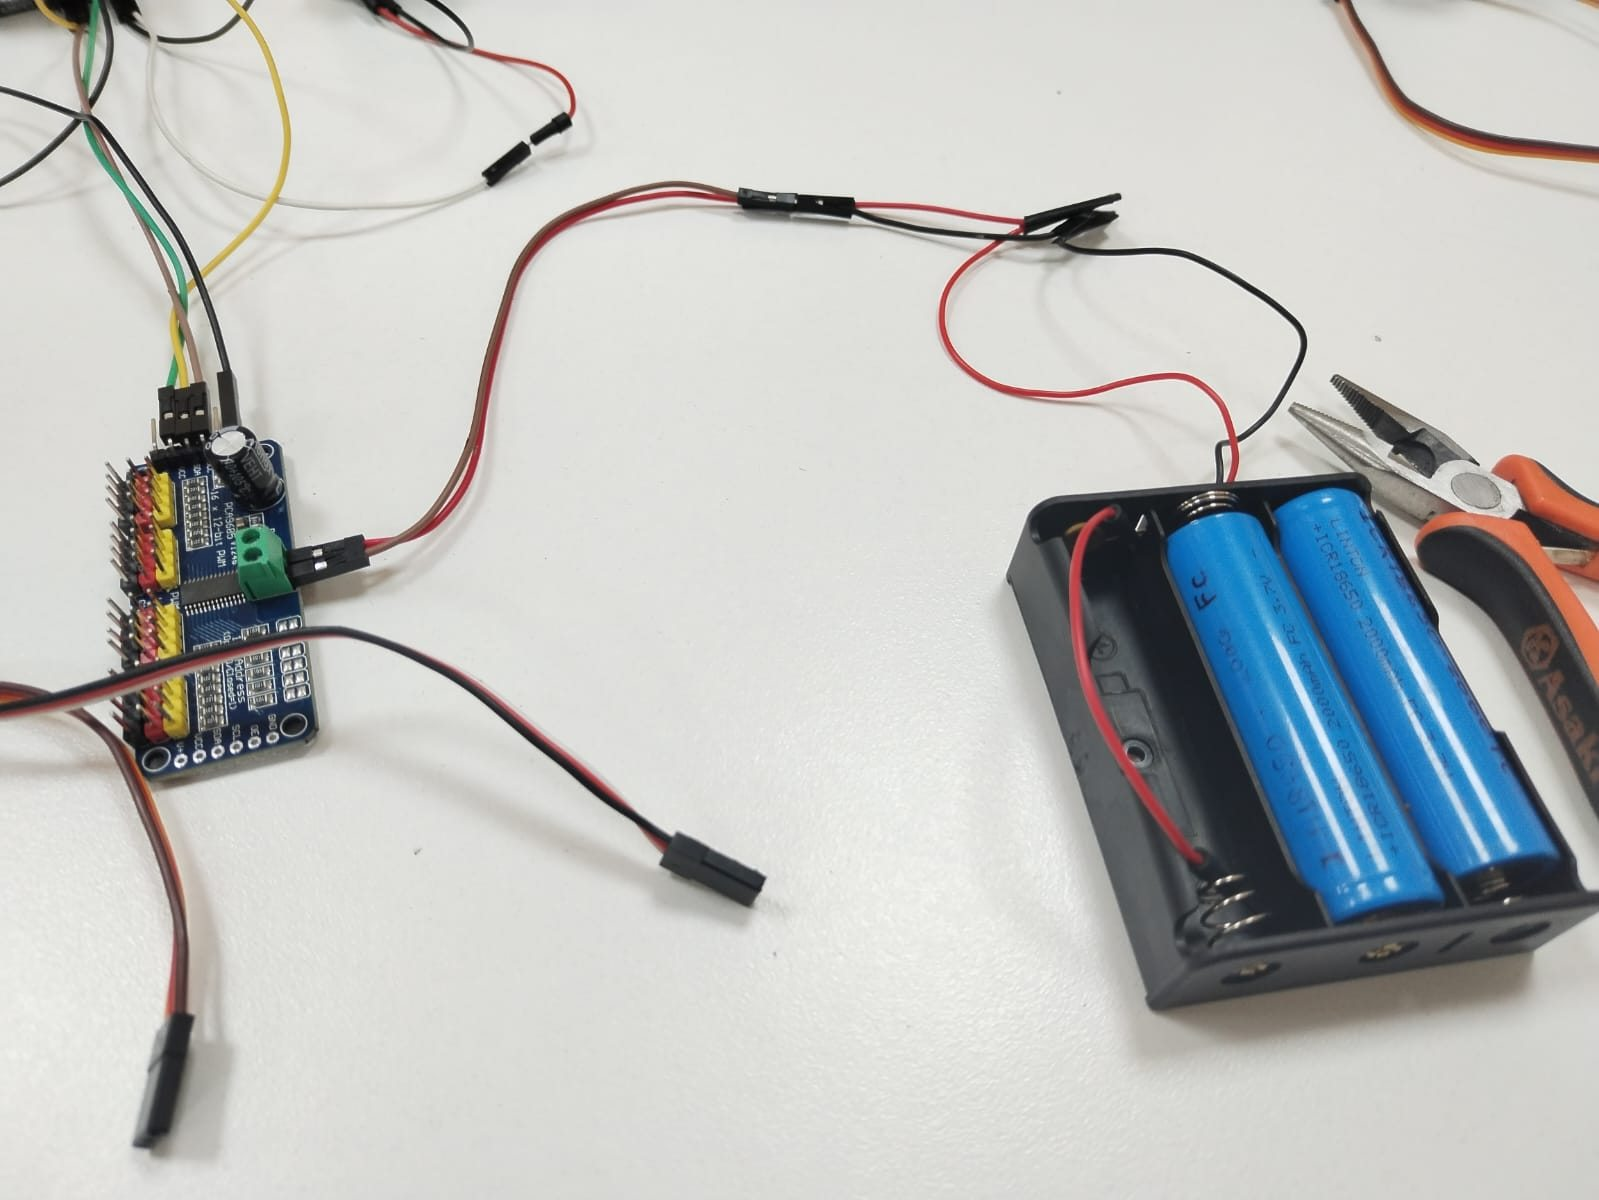
\includegraphics[width=\linewidth,height=7cm,keepaspectratio]{img/evidencia_portapilas_pca9685.jpg}
  \caption{Portapilas de dos celdas junto al PCA9685.}
 \end{subfigure}\hfill
 \begin{subfigure}[t]{0.48\textwidth}
  \centering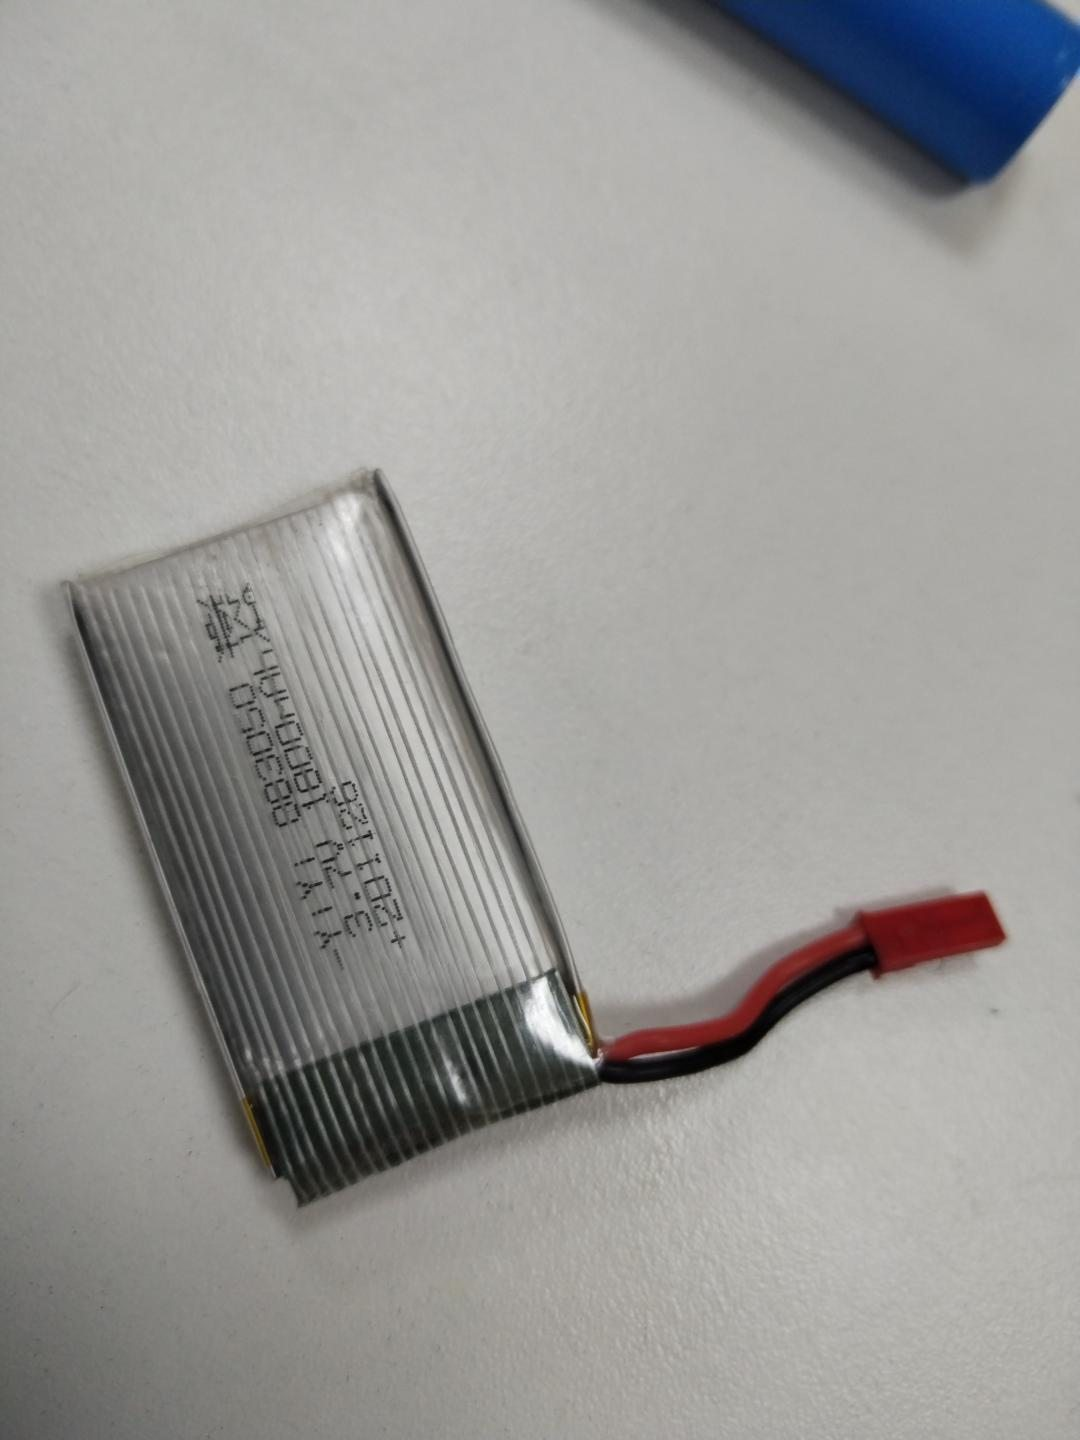
\includegraphics[width=\linewidth,height=7cm,keepaspectratio]{img/evidencia_bateria_lipo.jpg}
  \caption{Batería recargable plana observada en el laboratorio.}
 \end{subfigure}
 \caption{Alternativas de alimentación fotografiadas durante la integración.}
 \label{fig:actualizacion_fuentes}
\end{figure}

Es imprescindible separar la alimentación lógica del ESP32 de la alimentación de potencia de los actuadores, mantener una referencia GND común donde corresponda y utilizar una fuente con corriente suficiente para los picos de los servos. Las baterías de litio requieren protección adecuada contra cortocircuitos, sobrecorriente y descarga excesiva. La desactivación PWM por software no equivale a un interruptor físico de emergencia.

\subsection{Verificación de comunicación local mediante Wi-Fi}
En una captura previa, el teléfono aparece conectado a una red identificada como \texttt{FRANKI-HE}, sin acceso a Internet. Esto es compatible con un funcionamiento en red local: un punto de acceso puede permitir comunicación con dispositivos conectados sin ofrecer salida a Internet. Una segunda captura muestra la dirección privada \texttt{192.168.4.1} con una interfaz web de configuración de la cámara OV2640, incluyendo resolución QVGA (320$\times$240) y controles de exposición, brillo y contraste. Esta captura es evidencia del acceso HTTP a una interfaz de cámara en la red local, aunque no prueba el funcionamiento del panel de servos documentado en el código principal. También debe señalarse que el SSID observado, \texttt{FRANKI-HE}, no coincide con el SSID \texttt{Brazo-ESP32CAM} configurado en la versión revisada de \texttt{brazoR.ino}, por lo que podría corresponder a otra configuración o versión de prueba.

\begin{figure}[H]
 \centering
 \begin{subfigure}[t]{0.48\textwidth}
  \centering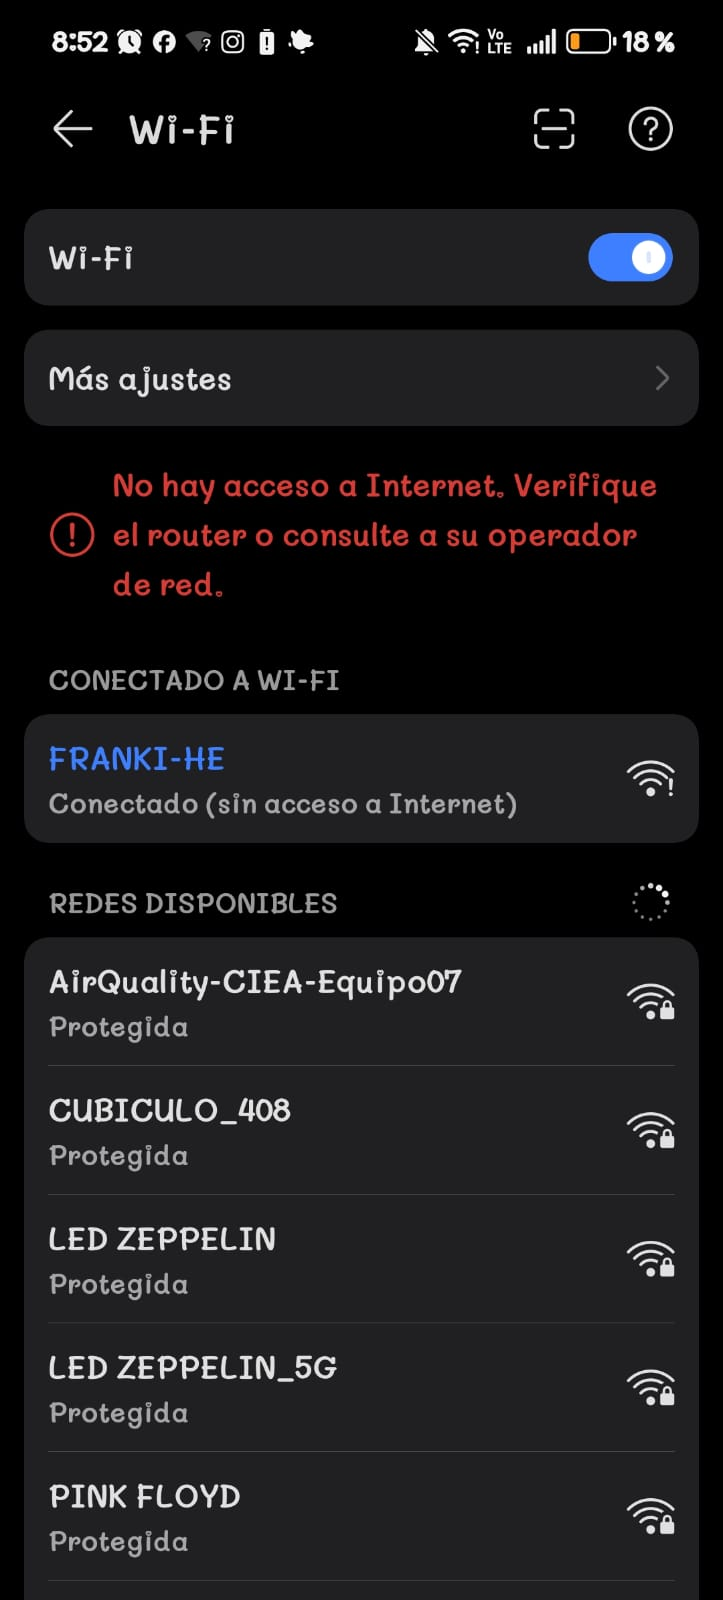
\includegraphics[width=\linewidth,height=9cm,keepaspectratio]{img/evidencia_wifi_red_local.png}
  \caption{Red local \texttt{FRANKI-HE} conectada.}
 \end{subfigure}\hfill
 \begin{subfigure}[t]{0.48\textwidth}
  \centering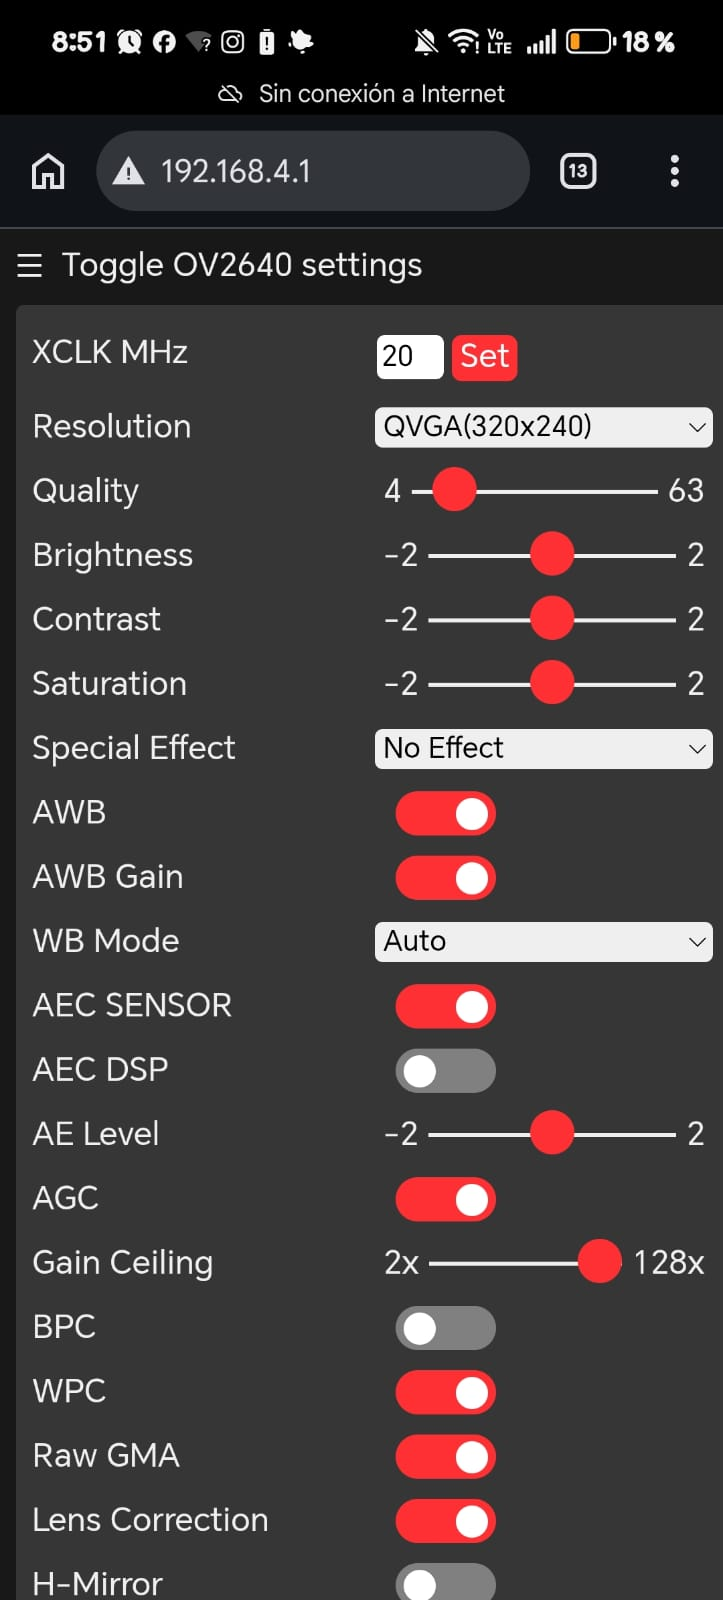
\includegraphics[width=\linewidth,height=9cm,keepaspectratio]{img/evidencia_wifi_panel_ov2640.png}
  \caption{Interfaz OV2640 en \texttt{192.168.4.1}.}
 \end{subfigure}
 \caption{Evidencias de comunicación inalámbrica y acceso web desde un dispositivo móvil.}
 \label{fig:actualizacion_wifi}
\end{figure}

\subsection{Procedimiento de calibración y comprobaciones pendientes}
Para pasar del ensamblaje observado a una calibración verificable se propone: (i) desenergizar y asegurar mecánicamente las uniones; (ii) confirmar el apriete de los servocuernos y la ausencia de holguras; (iii) alimentar un solo servo con una fuente medida y adecuada; (iv) comprobar el centro nominal de $90^\circ$ antes de fijar el eslabón; (v) recorrer gradualmente los límites evitando topes; y (vi) repetir el procedimiento articulación por articulación. El programa del repositorio utiliza límites nominales de $30^\circ$ a $150^\circ$ y debe ajustarse según el espacio mecánico real.

\begin{table}[H]
\centering\small
\caption{Registro de verificaciones y estado de evidencia disponible}
\label{tab:actualizacion_verificaciones}
\begin{tabularx}{\textwidth}{p{4.0cm} X p{3.2cm}}
\toprule
\textbf{Elemento} & \textbf{Evidencia o criterio} & \textbf{Estado documentado}\\
\midrule
Montaje de eslabones & Fotografías del brazo en varias posturas. & Observado\\
Controlador PCA9685 & Fotografías del módulo y del cableado. & Montaje observado\\
Comunicación Wi-Fi & Capturas de red local e interfaz OV2640. & Acceso web observado\\
Tensión de alimentación & Lectura con multímetro y polaridad. & Sin medida aportada\\
Ángulos reales & Comparación entre orden y medición física. & Sin medida aportada\\
Movimiento de seis servos & Ensayo individual con registro de resultados. & No demostrado por las fotos\\
\bottomrule
\end{tabularx}
\end{table}

\subsection{Balance del avance experimental}
Respecto a la documentación previa, las fotografías aportan evidencia adicional de integración física del brazo, presencia de cableado electrónico, disposición del PCA9685, inspección de alimentaciones y acceso a una interfaz web local. Sin embargo, sería incorrecto transformar estas observaciones en resultados cuantitativos de exactitud o autonomía sin mediciones. Como siguiente etapa se recomienda anexar una tabla con tensión de alimentación en reposo y bajo carga, lectura de corriente, posición angular ordenada y observada para cada articulación, y resultado de las pruebas de comunicación y movimiento.

% Usa paquetes ya presentes en main.tex: graphicx, float, booktabs, tabularx, subcaption.

\section{Actualización experimental: ensamble, conexiones y ajustes del manipulador}
\label{sec:actualizacion_evidencias}

\subsection{Objeto y alcance del registro fotográfico}
Las evidencias recopiladas corresponden a una nueva etapa de integración del brazo robótico articulado. Se observan diferentes configuraciones mecánicas del manipulador, el montaje de un controlador PWM PCA9685, un módulo de la familia ESP32, conexiones mediante cables y elementos empleados para evaluar la alimentación eléctrica. El propósito de esta sección es registrar el progreso físico del prototipo y delimitar las comprobaciones que aún se requieren. Las fotografías son evidencia de montaje, pero no constituyen por sí mismas una medida de precisión, par disponible o estabilidad eléctrica.

\subsection{Progreso del ensamblaje y postura de las articulaciones}
El manipulador conserva una estructura de eslabones rígidos, servomotores montados en soportes metálicos, pinza mecánica y base de madera. Las nuevas imágenes muestran posiciones inclinadas, frontales y casi verticales, útiles para observar la alineación relativa de hombro, codo y muñeca. Estas posiciones sirven como referencia para identificar posibles interferencias, puntos de holgura y distribución del cableado. No se dispone de un registro instrumental de los ángulos reales, por lo que la denominación ``calibración'' se emplea aquí para describir el proceso de ajuste y verificación, no para afirmar que haya concluido.

\begin{figure}[H]
 \centering
 \begin{subfigure}[t]{0.48\textwidth}
  \centering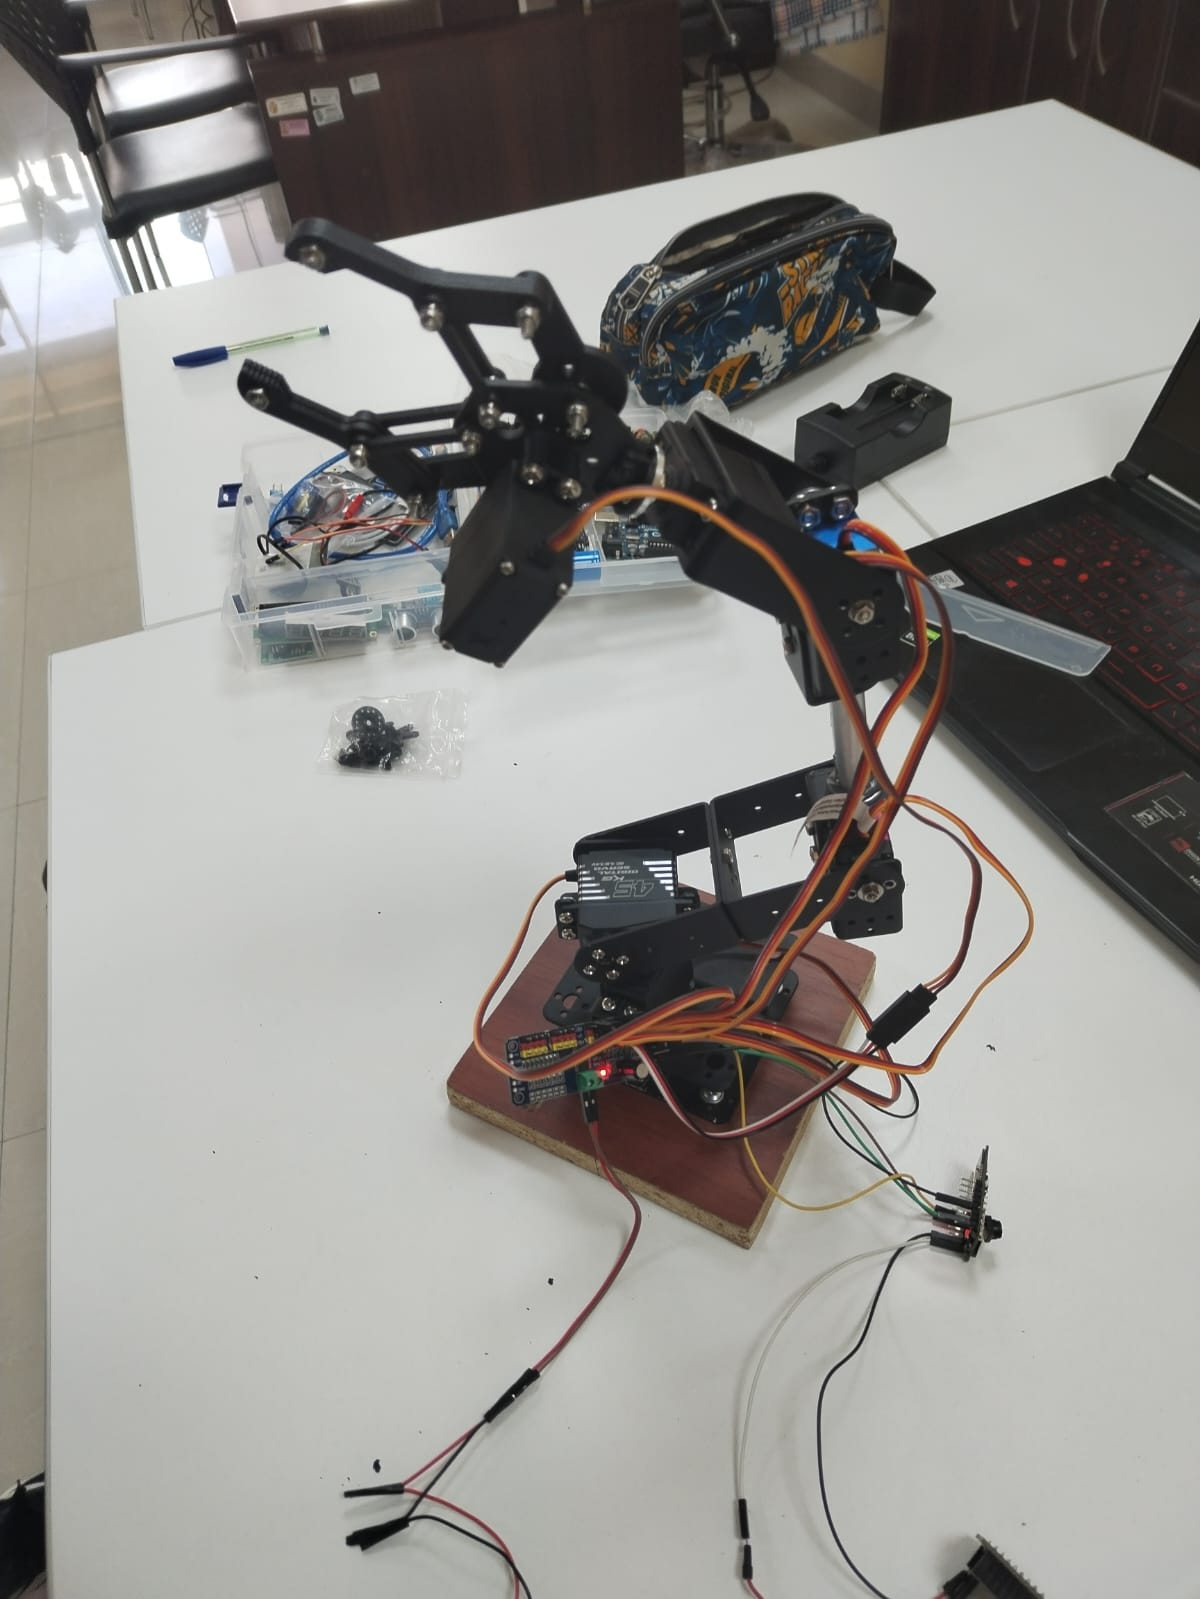
\includegraphics[width=\linewidth,height=7cm,keepaspectratio]{img/evidencia_brazo_integracion_lateral.jpg}
  \caption{Vista lateral durante la integración de la pinza y los eslabones.}
 \end{subfigure}\hfill
 \begin{subfigure}[t]{0.48\textwidth}
  \centering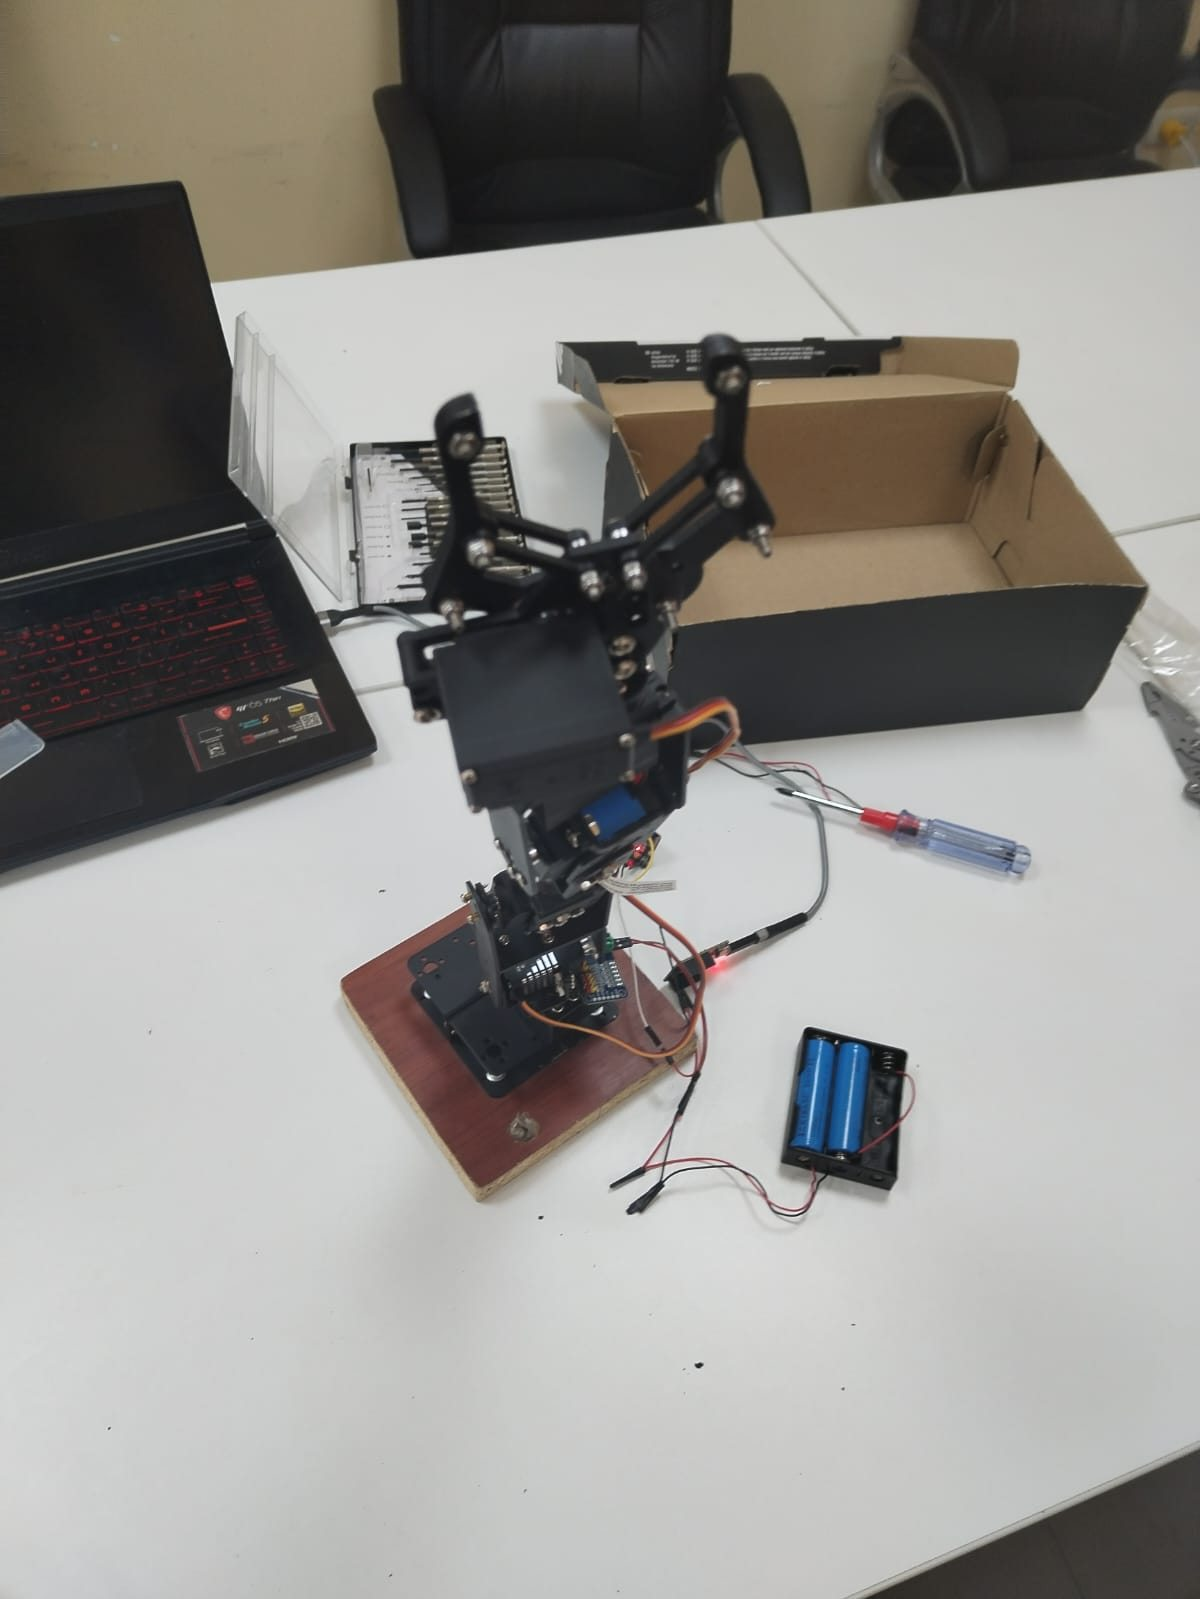
\includegraphics[width=\linewidth,height=7cm,keepaspectratio]{img/evidencia_brazo_vista_frontal.jpg}
  \caption{Vista frontal del conjunto articulado en banco de trabajo.}
 \end{subfigure}
 \caption{Registro del ensamble físico en diferentes orientaciones.}
 \label{fig:actualizacion_ensamble}
\end{figure}

\begin{figure}[H]
 \centering
 \begin{subfigure}[t]{0.48\textwidth}
  \centering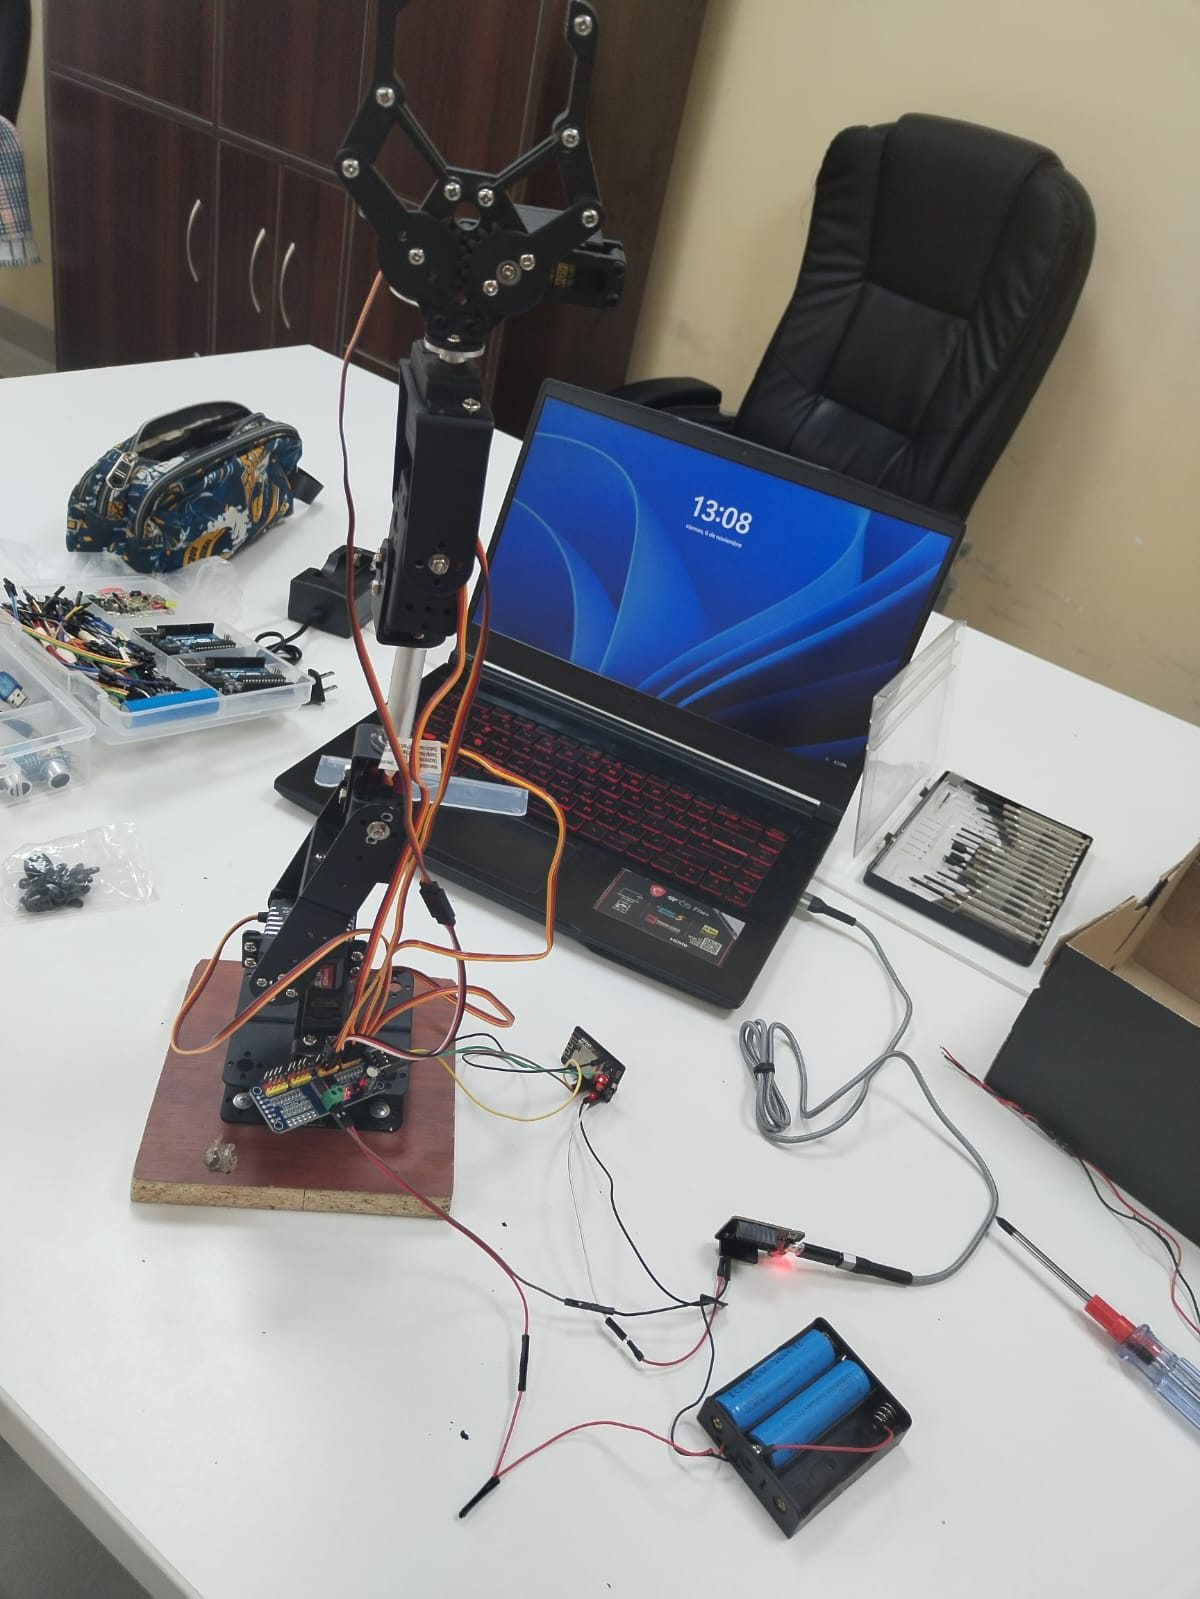
\includegraphics[width=\linewidth,height=7cm,keepaspectratio]{img/evidencia_brazo_postura_vertical.jpg}
  \caption{Prototipo con el efector final elevado.}
 \end{subfigure}\hfill
 \begin{subfigure}[t]{0.48\textwidth}
  \centering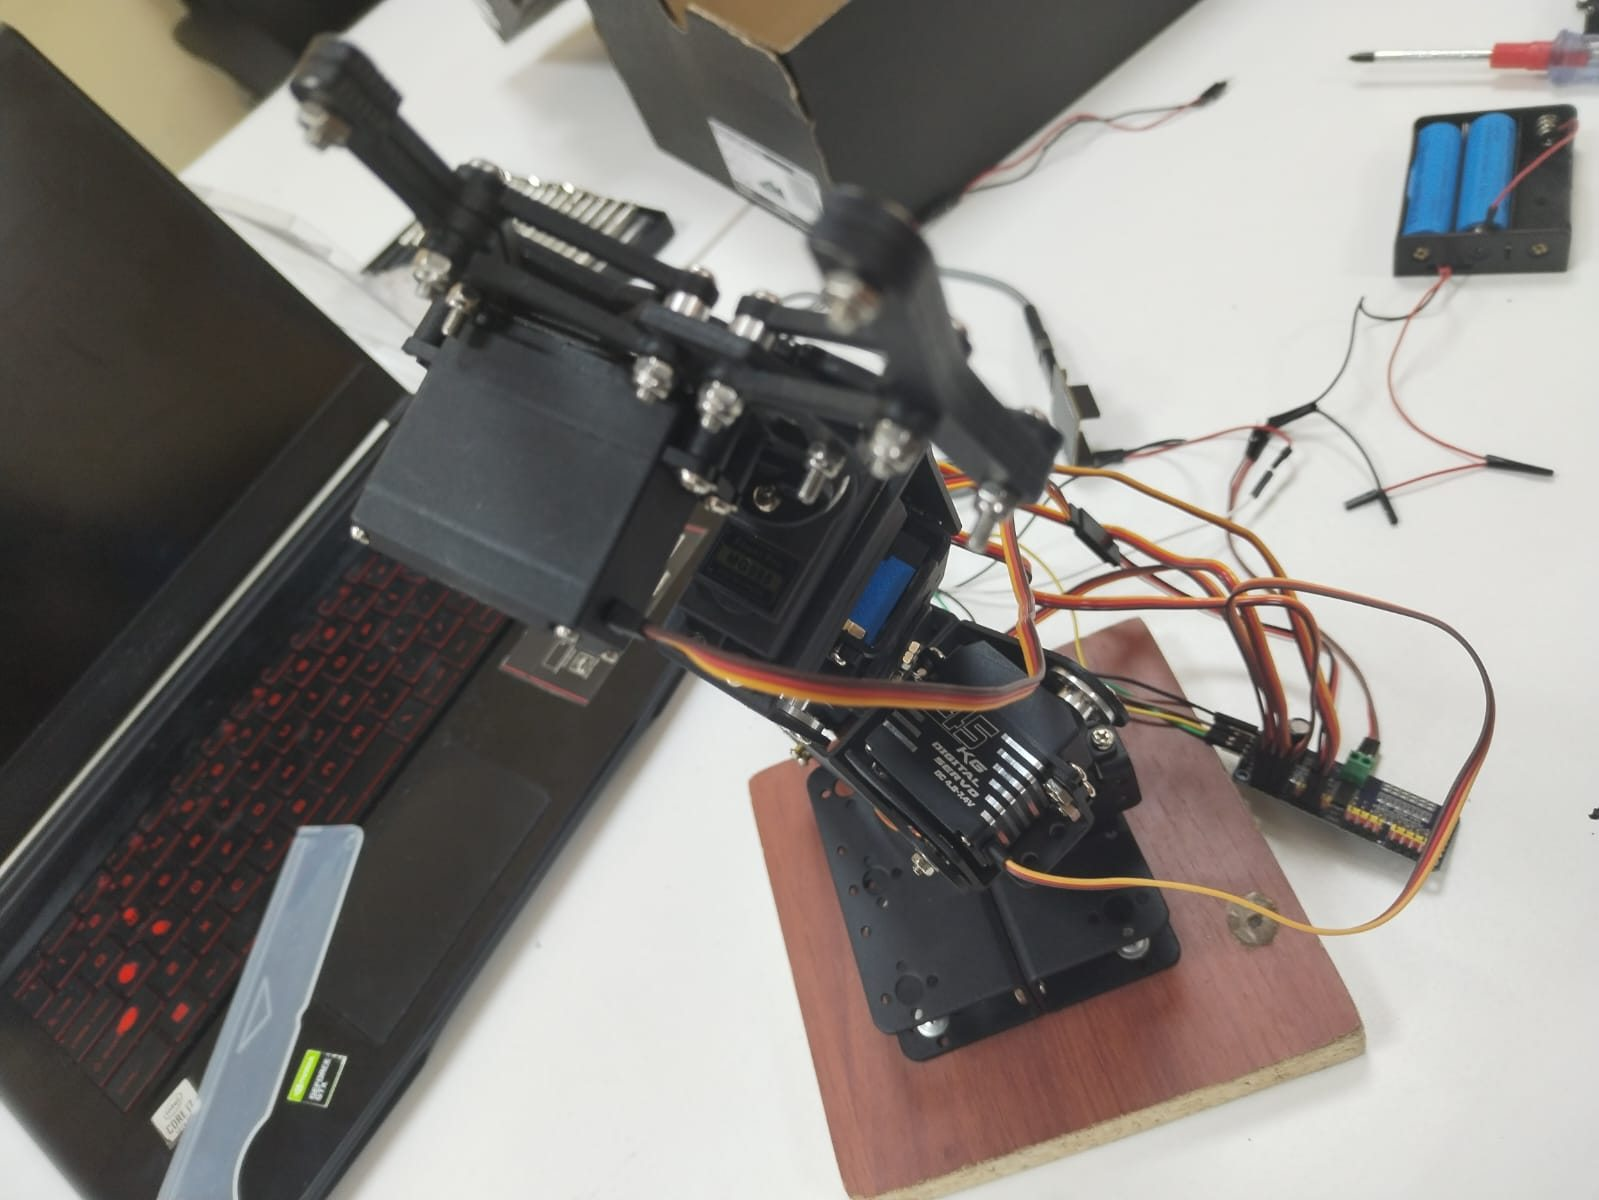
\includegraphics[width=\linewidth,height=7cm,keepaspectratio]{img/evidencia_brazo_articulaciones_closeup.jpg}
  \caption{Detalle de los soportes y uniones cercanos a la pinza.}
 \end{subfigure}
 \caption{Posturas de referencia para la revisión de alineación y holguras.}
 \label{fig:actualizacion_posturas}
\end{figure}

\begin{figure}[H]
 \centering
 \begin{subfigure}[t]{0.48\textwidth}
  \centering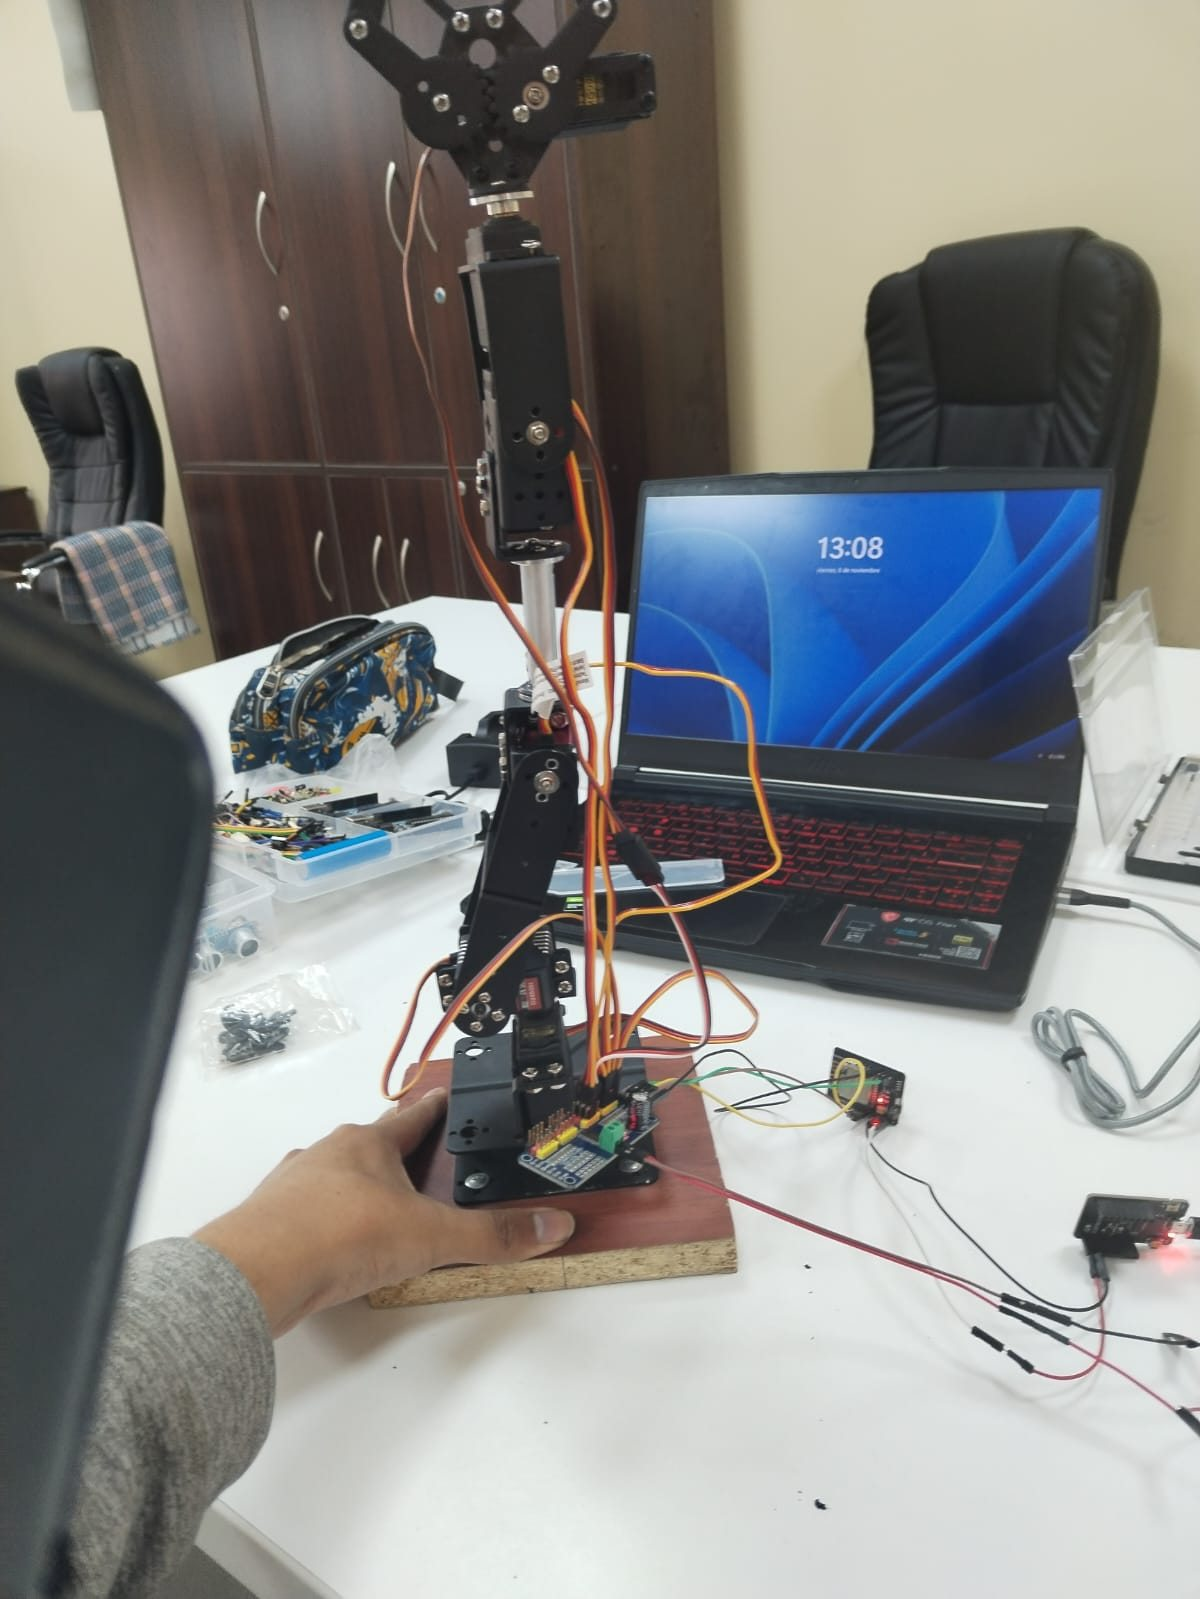
\includegraphics[width=\linewidth,height=7cm,keepaspectratio]{img/evidencia_brazo_estabilidad_base.jpg}
  \caption{Sujeción manual del conjunto a su base.}
 \end{subfigure}\hfill
 \begin{subfigure}[t]{0.48\textwidth}
  \centering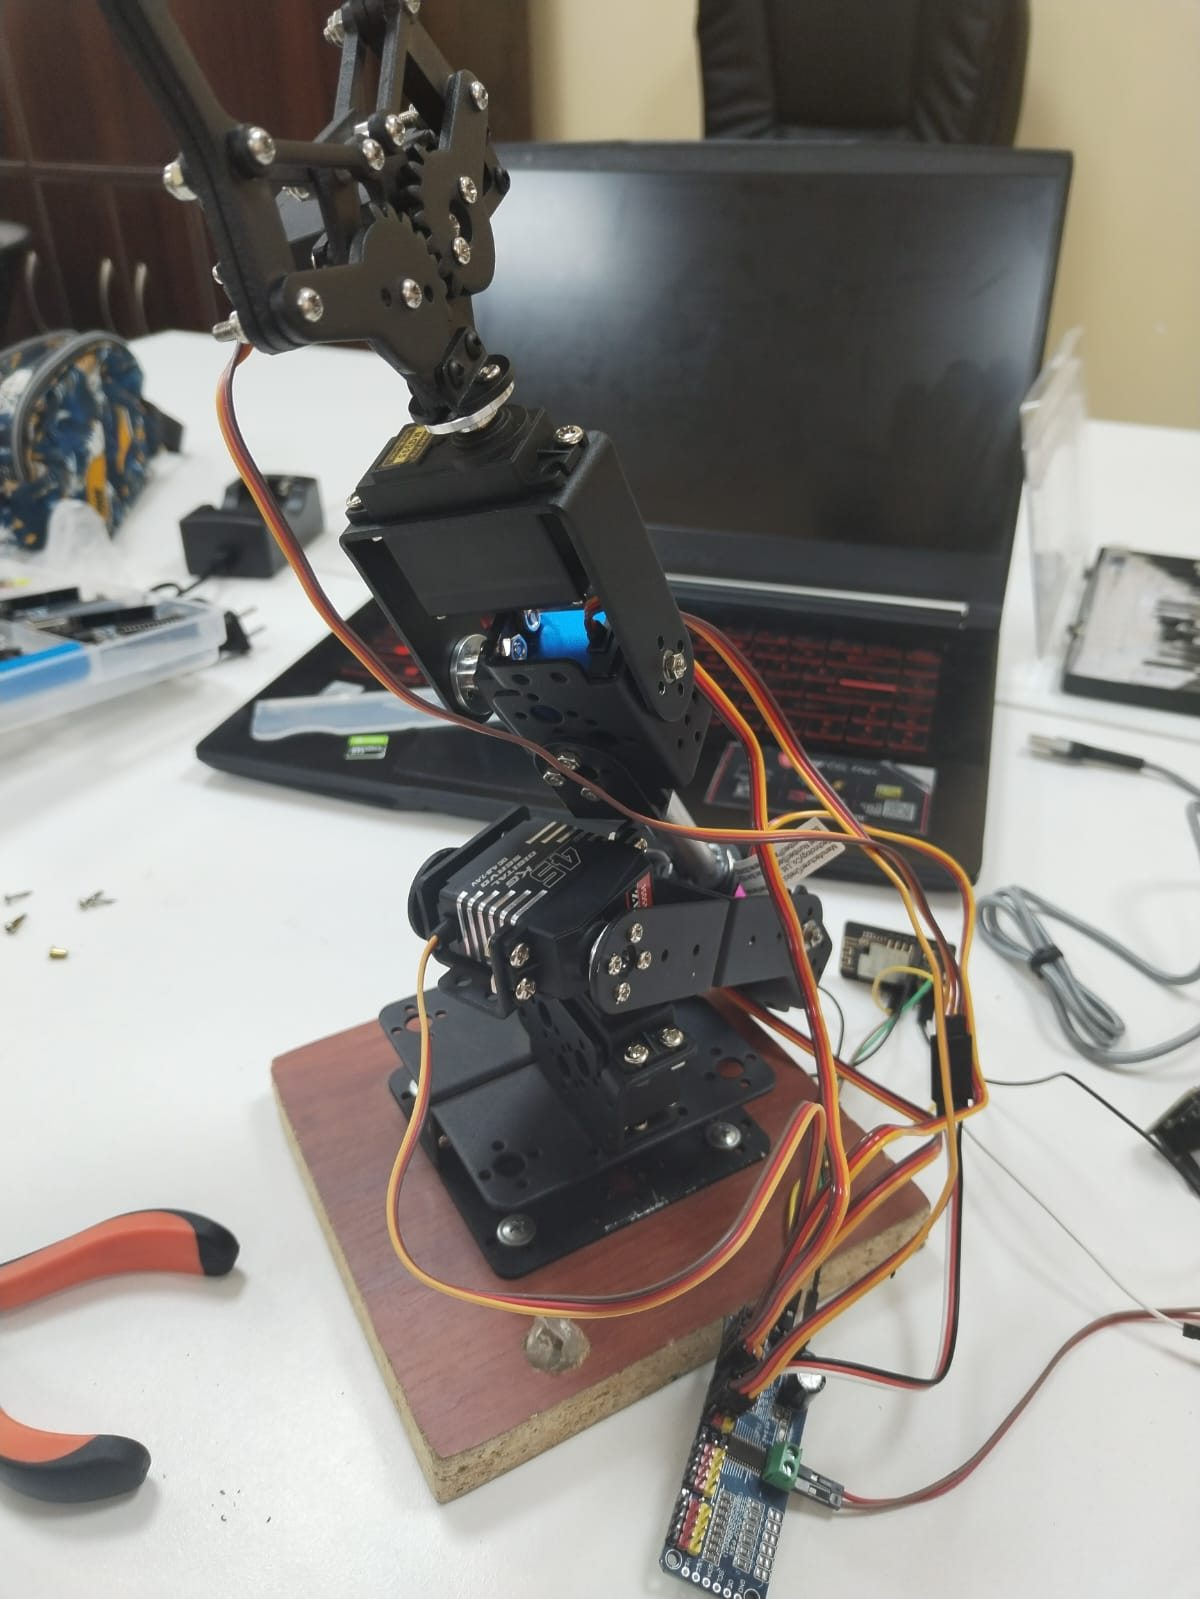
\includegraphics[width=\linewidth,height=7cm,keepaspectratio]{img/evidencia_brazo_soportes_mecanicos.jpg}
  \caption{Vista cercana de servomotores, soportes y tornillería.}
 \end{subfigure}
 \caption{Inspección mecánica de las articulaciones y la plataforma soporte.}
 \label{fig:actualizacion_base}
\end{figure}

\subsection{Integración del ESP32 y del controlador PCA9685}
En las imágenes se reconoce el módulo PCA9685, cuyas cabeceras distribuyen las señales de control hacia los servomotores. El controlador recibe las órdenes por el bus $I^2C$ y genera las señales PWM independientemente del procesador. La fotografía del cableado permite observar conexiones entre módulos, aunque no basta para certificar continuidad, polaridad o asignación exacta de cada conductor. En el firmware del repositorio se configuran de forma nominal SDA en GPIO 13, SCL en GPIO 14 y dirección $I^2C$ \texttt{0x40}; estos valores deben contrastarse con el montaje realmente utilizado.

\begin{figure}[H]
 \centering
 \begin{subfigure}[t]{0.48\textwidth}
  \centering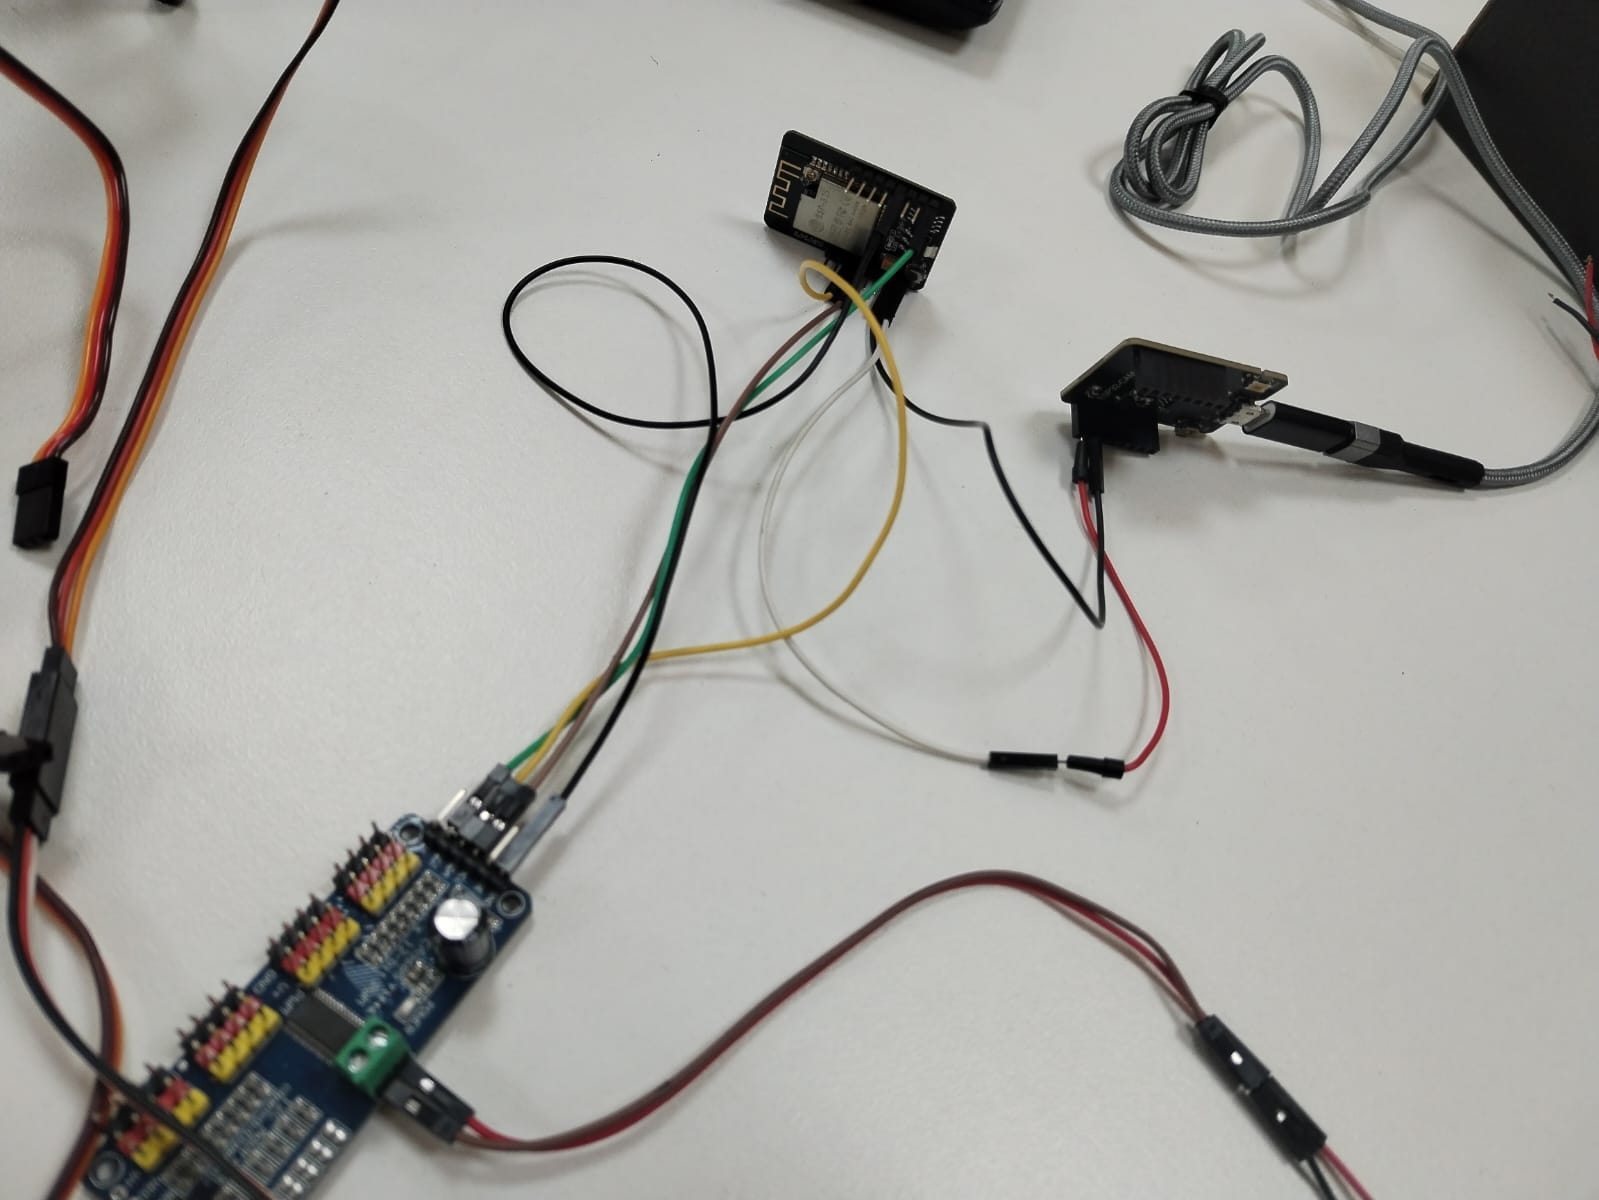
\includegraphics[width=\linewidth,height=7cm,keepaspectratio]{img/evidencia_esp32_pca9685_cableado.jpg}
  \caption{Módulos electrónicos y conductores de interconexión.}
 \end{subfigure}\hfill
 \begin{subfigure}[t]{0.48\textwidth}
  \centering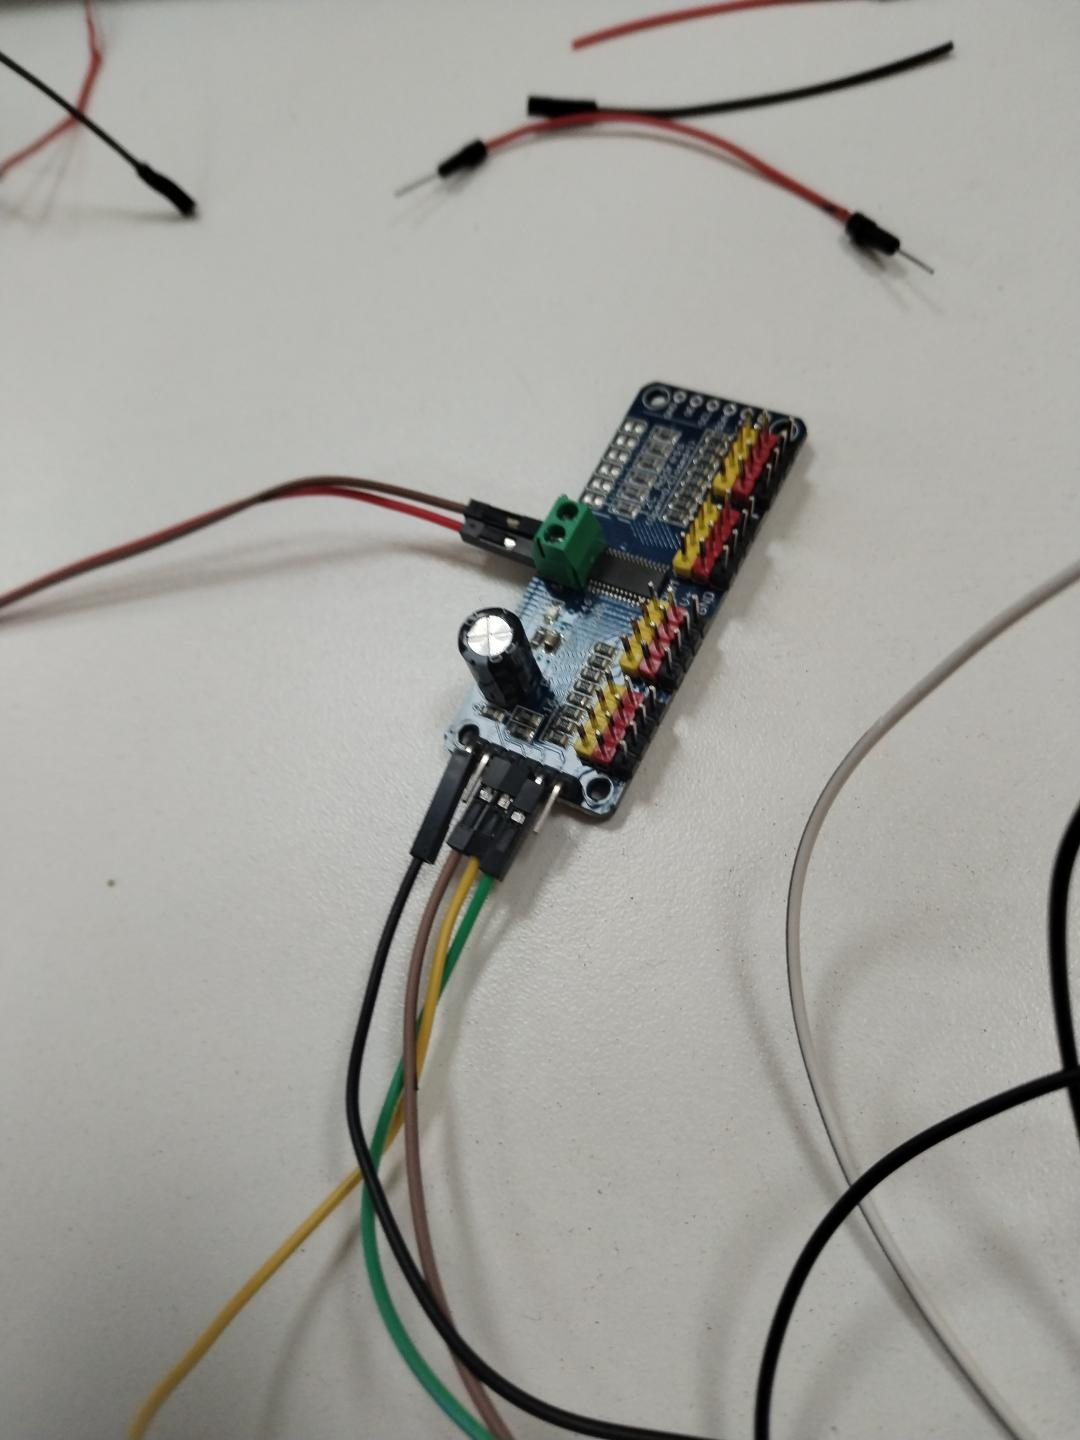
\includegraphics[width=\linewidth,height=7cm,keepaspectratio]{img/evidencia_pca9685_detalle.jpg}
  \caption{Vista cercana del PCA9685 y su bornera.}
 \end{subfigure}
 \caption{Evidencia de avance en la integración del sistema de control electrónico.}
 \label{fig:actualizacion_pca}
\end{figure}

Para validar esta etapa se propone realizar una lectura del bus $I^2C$ con el programa de escaneo del repositorio y registrar el resultado en el monitor serie. Una detección de \texttt{0x40} demostraría comunicación digital con el controlador, pero no permitiría concluir por sí sola que los servomotores estén bien alimentados o que su movimiento sea seguro.

\subsection{Revisión de fuentes de alimentación y baterías}
Las evidencias incluyen un portapilas con dos celdas cilíndricas y una batería plana recargable. Su presencia documenta la evaluación de alternativas de alimentación; no se puede establecer a partir de las fotografías cuál fue conectada durante cada ensayo ni verificar su tensión, capacidad efectiva o corriente disponible. Antes de suministrar energía al riel de servomotores se debe medir la salida con un multímetro y comprobar que la tensión resultante no supere la admisible para el conjunto de servos empleado. No debe asumirse que dos celdas tienen una tensión determinada sin conocer su conexión serie/paralelo y su estado de carga.

\begin{figure}[H]
 \centering
 \begin{subfigure}[t]{0.48\textwidth}
  \centering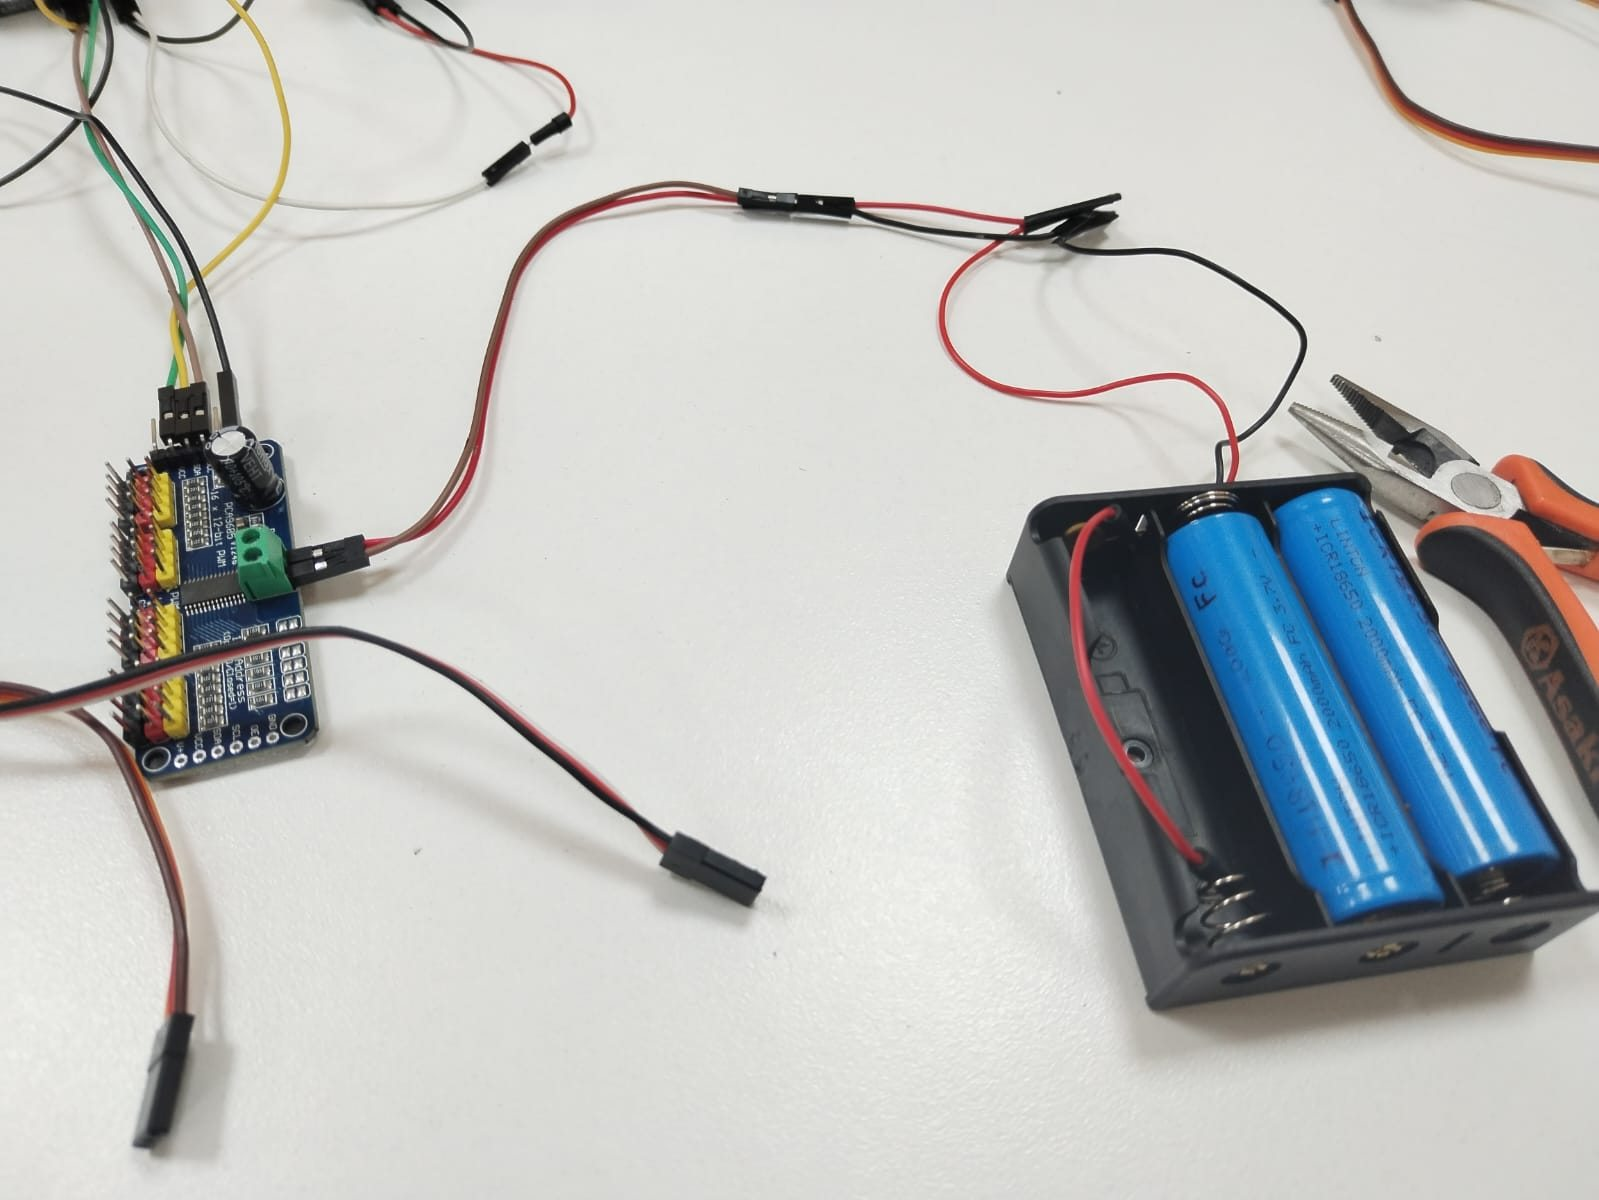
\includegraphics[width=\linewidth,height=7cm,keepaspectratio]{img/evidencia_portapilas_pca9685.jpg}
  \caption{Portapilas de dos celdas junto al PCA9685.}
 \end{subfigure}\hfill
 \begin{subfigure}[t]{0.48\textwidth}
  \centering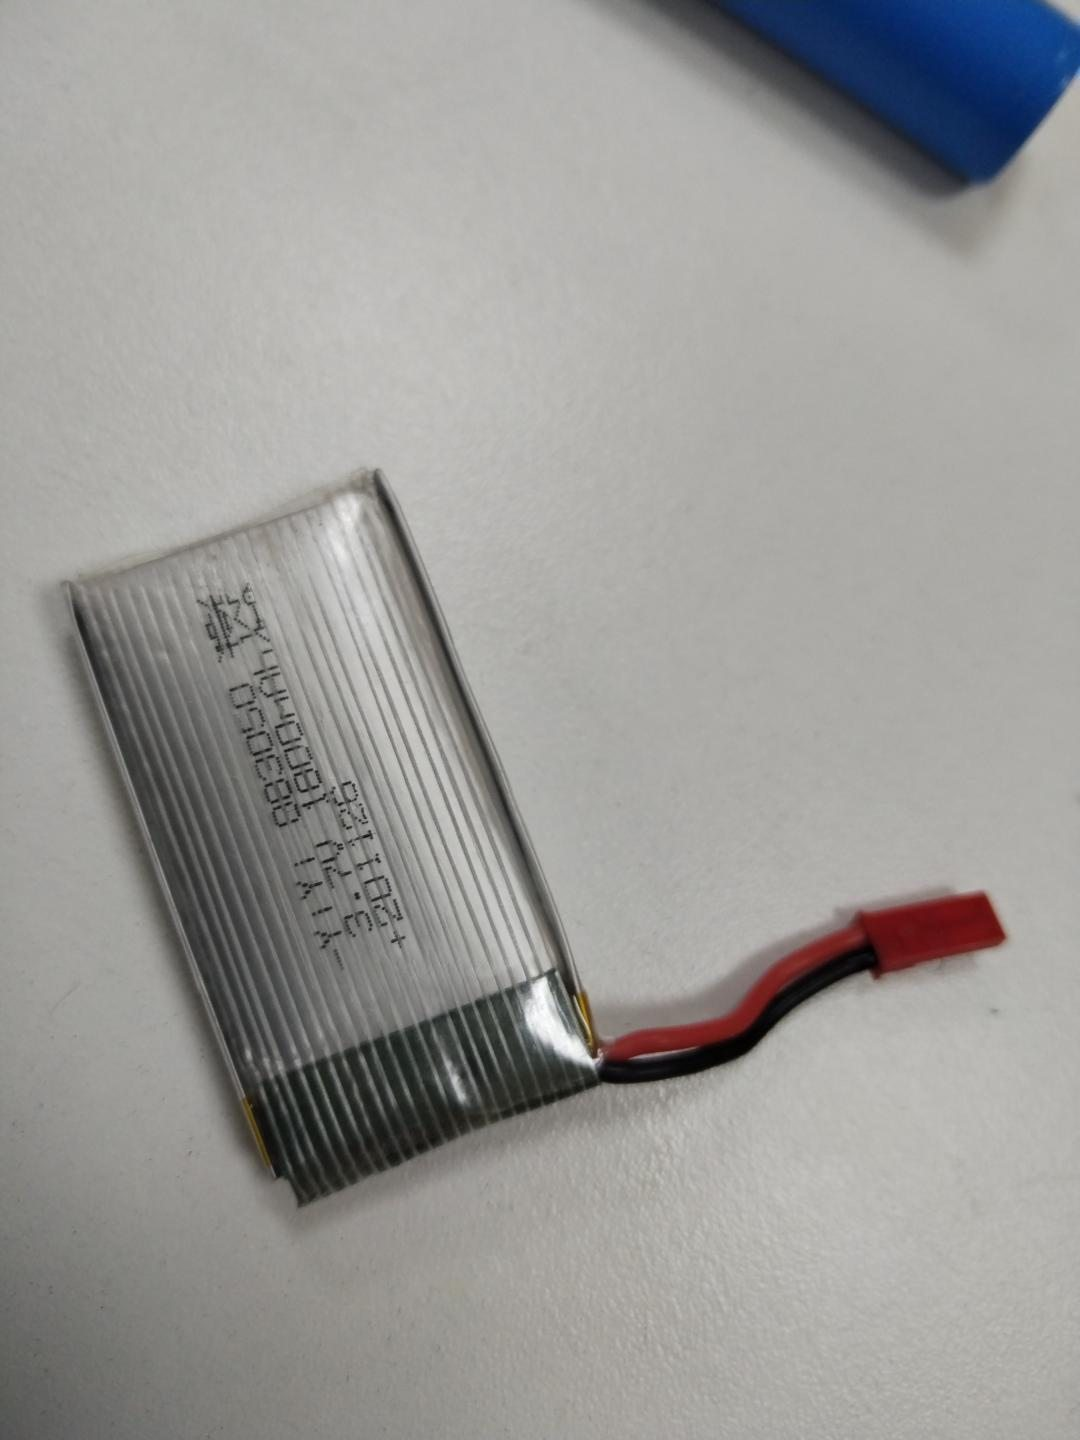
\includegraphics[width=\linewidth,height=7cm,keepaspectratio]{img/evidencia_bateria_lipo.jpg}
  \caption{Batería recargable plana observada en el laboratorio.}
 \end{subfigure}
 \caption{Alternativas de alimentación fotografiadas durante la integración.}
 \label{fig:actualizacion_fuentes}
\end{figure}

Es imprescindible separar la alimentación lógica del ESP32 de la alimentación de potencia de los actuadores, mantener una referencia GND común donde corresponda y utilizar una fuente con corriente suficiente para los picos de los servos. Las baterías de litio requieren protección adecuada contra cortocircuitos, sobrecorriente y descarga excesiva. La desactivación PWM por software no equivale a un interruptor físico de emergencia.

\subsection{Verificación de comunicación local mediante Wi-Fi}
En una captura previa, el teléfono aparece conectado a una red identificada como \texttt{FRANKI-HE}, sin acceso a Internet. Esto es compatible con un funcionamiento en red local: un punto de acceso puede permitir comunicación con dispositivos conectados sin ofrecer salida a Internet. Una segunda captura muestra la dirección privada \texttt{192.168.4.1} con una interfaz web de configuración de la cámara OV2640, incluyendo resolución QVGA (320$\times$240) y controles de exposición, brillo y contraste. Esta captura es evidencia del acceso HTTP a una interfaz de cámara en la red local, aunque no prueba el funcionamiento del panel de servos documentado en el código principal. También debe señalarse que el SSID observado, \texttt{FRANKI-HE}, no coincide con el SSID \texttt{Brazo-ESP32CAM} configurado en la versión revisada de \texttt{brazoR.ino}, por lo que podría corresponder a otra configuración o versión de prueba.

\begin{figure}[H]
 \centering
 \begin{subfigure}[t]{0.48\textwidth}
  \centering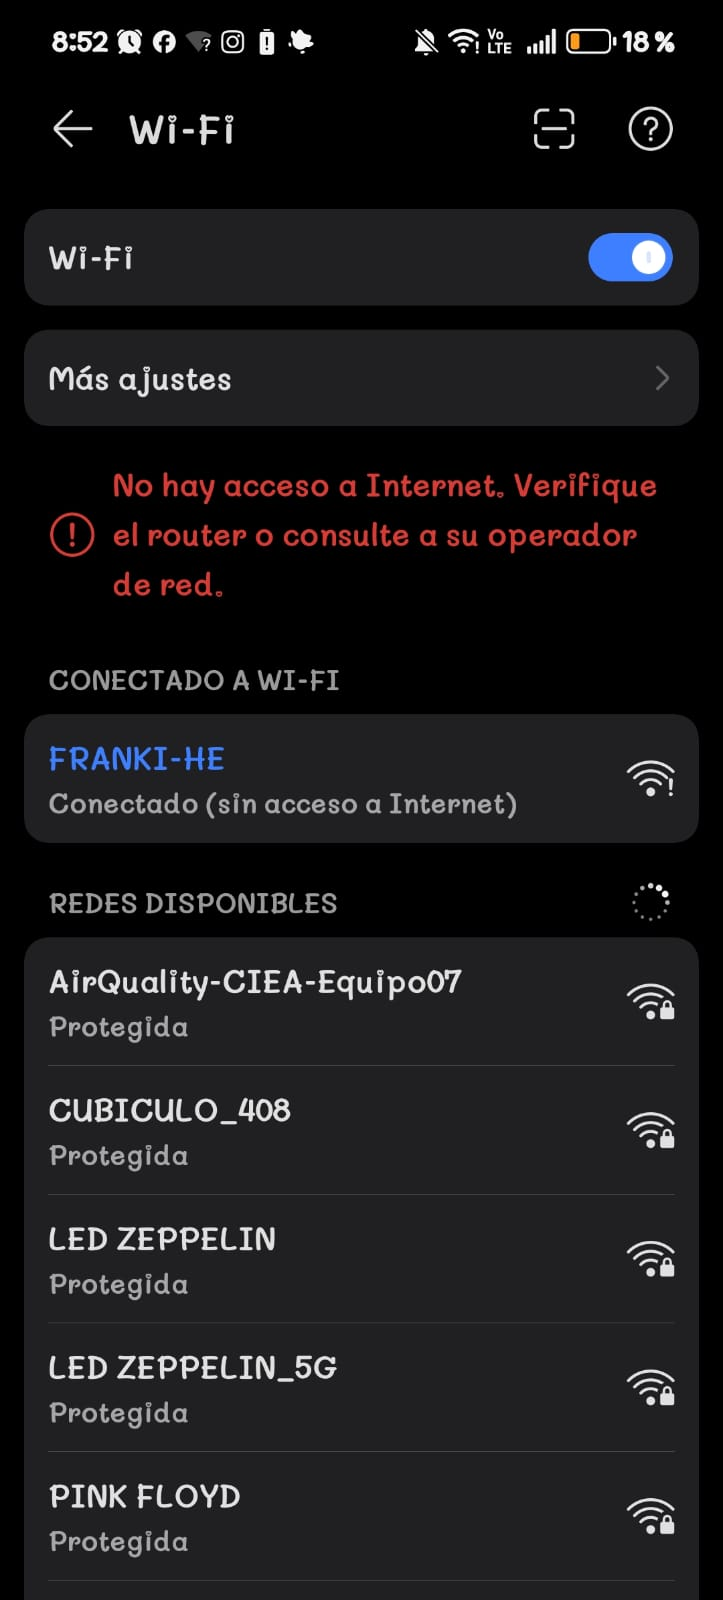
\includegraphics[width=\linewidth,height=9cm,keepaspectratio]{img/evidencia_wifi_red_local.png}
  \caption{Red local \texttt{FRANKI-HE} conectada.}
 \end{subfigure}\hfill
 \begin{subfigure}[t]{0.48\textwidth}
  \centering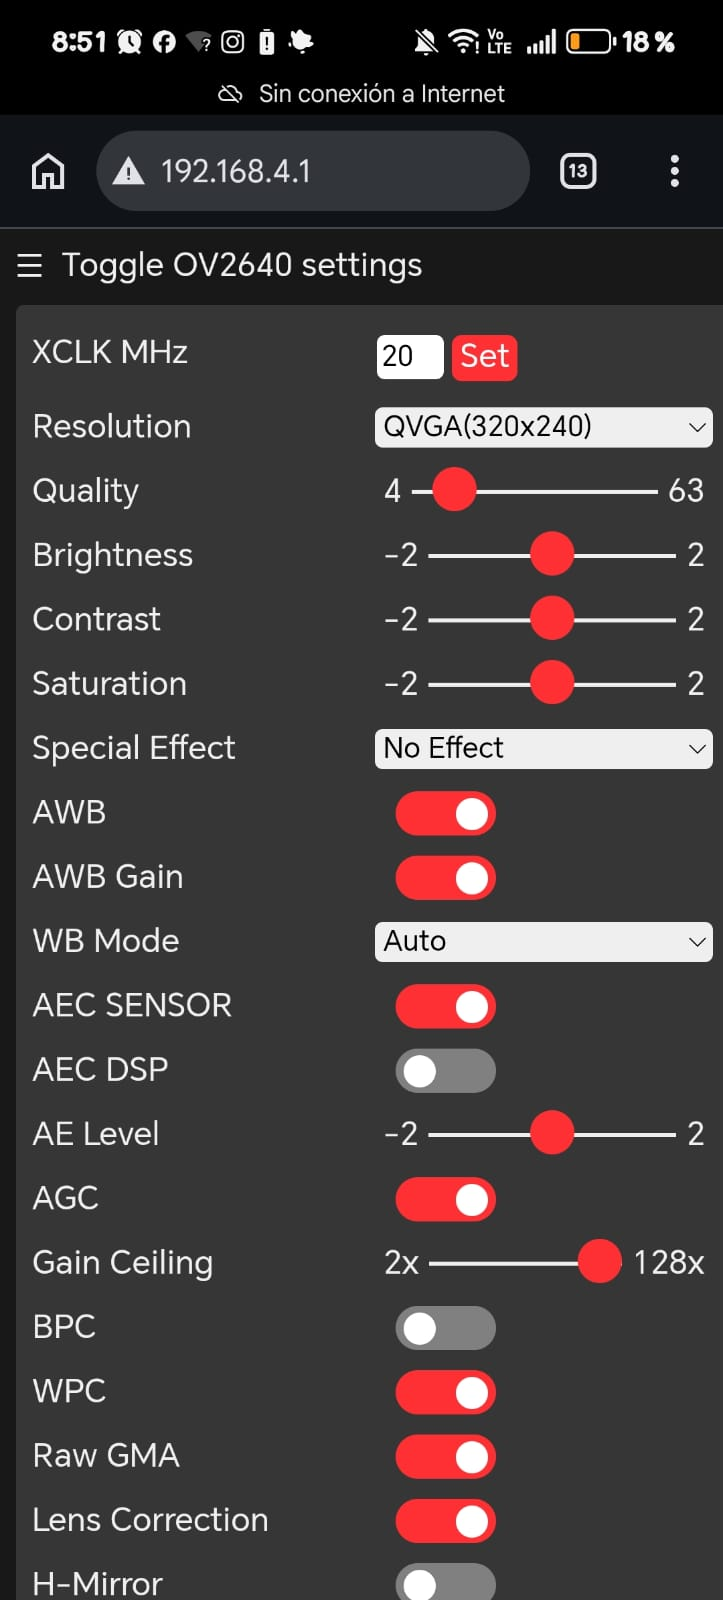
\includegraphics[width=\linewidth,height=9cm,keepaspectratio]{img/evidencia_wifi_panel_ov2640.png}
  \caption{Interfaz OV2640 en \texttt{192.168.4.1}.}
 \end{subfigure}
 \caption{Evidencias de comunicación inalámbrica y acceso web desde un dispositivo móvil.}
 \label{fig:actualizacion_wifi}
\end{figure}

\subsection{Procedimiento de calibración y comprobaciones pendientes}
Para pasar del ensamblaje observado a una calibración verificable se propone: (i) desenergizar y asegurar mecánicamente las uniones; (ii) confirmar el apriete de los servocuernos y la ausencia de holguras; (iii) alimentar un solo servo con una fuente medida y adecuada; (iv) comprobar el centro nominal de $90^\circ$ antes de fijar el eslabón; (v) recorrer gradualmente los límites evitando topes; y (vi) repetir el procedimiento articulación por articulación. El programa del repositorio utiliza límites nominales de $30^\circ$ a $150^\circ$ y debe ajustarse según el espacio mecánico real.

\begin{table}[H]
\centering\small
\caption{Registro de verificaciones y estado de evidencia disponible}
\label{tab:actualizacion_verificaciones}
\begin{tabularx}{\textwidth}{p{4.0cm} X p{3.2cm}}
\toprule
\textbf{Elemento} & \textbf{Evidencia o criterio} & \textbf{Estado documentado}\\
\midrule
Montaje de eslabones & Fotografías del brazo en varias posturas. & Observado\\
Controlador PCA9685 & Fotografías del módulo y del cableado. & Montaje observado\\
Comunicación Wi-Fi & Capturas de red local e interfaz OV2640. & Acceso web observado\\
Tensión de alimentación & Lectura con multímetro y polaridad. & Sin medida aportada\\
Ángulos reales & Comparación entre orden y medición física. & Sin medida aportada\\
Movimiento de seis servos & Ensayo individual con registro de resultados. & No demostrado por las fotos\\
\bottomrule
\end{tabularx}
\end{table}

\subsection{Balance del avance experimental}
Respecto a la documentación previa, las fotografías aportan evidencia adicional de integración física del brazo, presencia de cableado electrónico, disposición del PCA9685, inspección de alimentaciones y acceso a una interfaz web local. Sin embargo, sería incorrecto transformar estas observaciones en resultados cuantitativos de exactitud o autonomía sin mediciones. Como siguiente etapa se recomienda anexar una tabla con tensión de alimentación en reposo y bajo carga, lectura de corriente, posición angular ordenada y observada para cada articulación, y resultado de las pruebas de comunicación y movimiento.
